\input{"preamble.tex"}

\addbibresource{UGA\_Algebra\_Qual\_Questions.bib}

\let\Begin\begin
\let\End\end
\newcommand\wrapenv[1]{#1}

\makeatletter
\def\ScaleWidthIfNeeded{%
 \ifdim\Gin@nat@width>\linewidth
    \linewidth
  \else
    \Gin@nat@width
  \fi
}
\def\ScaleHeightIfNeeded{%
  \ifdim\Gin@nat@height>0.9\textheight
    0.9\textheight
  \else
    \Gin@nat@width
  \fi
}
\makeatother

\setkeys{Gin}{width=\ScaleWidthIfNeeded,height=\ScaleHeightIfNeeded,keepaspectratio}%

\title{
\textbf{
    UGA Algebra Qualifying Exam Questions (Spring 2011 -- Spring 2021)
  }
  }







\begin{document}

\date{}
\author{D. Zack Garza}
\maketitle


\newpage

% Note: addsec only in KomaScript
\addsec{Table of Contents}
\tableofcontents
\newpage

\hypertarget{group-theory-general}{%
\section{Group Theory: General}\label{group-theory-general}}

\hypertarget{spring-2020-2-work}{%
\subsection{\texorpdfstring{Spring 2020 \#2
\(\work\)}{Spring 2020 \#2 \textbackslash work}}\label{spring-2020-2-work}}

Let \(H\) be a normal subgroup of a finite group \(G\) where the order
of \(H\) and the index of \(H\) in \(G\) are relatively prime. Prove
that no other subgroup of \(G\) has the same order as \(H\).

\todo[inline]{Work this problem.}

\hypertarget{spring-2019-4-done}{%
\subsection{\texorpdfstring{Spring 2019 \#4
\(\done\)}{Spring 2019 \#4 \textbackslash done}}\label{spring-2019-4-done}}

For a finite group \(G\), let \(c(G)\) denote the number of conjugacy
classes of \(G\).

\begin{enumerate}
\def\labelenumi{\alph{enumi}.}
\item
  Prove that if two elements of \(G\) are chosen uniformly at
  random,then the probability they commute is precisely
  \begin{align*}
  \frac{c(G)}{{\left\lvert {G} \right\rvert}}
  .\end{align*}
\item
  State the class equation for a finite group.
\item
  Using the class equation (or otherwise) show that the probability in
  part (a) is at most
  \begin{align*}
  \frac 1 2 + \frac 1 {2[G : Z(G)]}
  .\end{align*}
\end{enumerate}

\begin{quote}
Here, as usual, \(Z(G)\) denotes the center of \(G\).
\end{quote}

\begin{concept}

\envlist

\begin{itemize}
\tightlist
\item
  Notation: \(X/G\) is the set of \(G{\hbox{-}}\)orbits
\item
  Notation:
  \(X^g = \left\{{x\in x{~\mathrel{\Big|}~}g\cdot x = x}\right\}\)
\item
  Burnside's formula:
  \({\left\lvert {G} \right\rvert} {\left\lvert {X/G} \right\rvert} = \sum {\left\lvert {X^g} \right\rvert}\).
\end{itemize}

\end{concept}

\begin{strategy}

Burnside.

\end{strategy}

\begin{solution}

\envlist

\begin{proof}[Part a]

Strategy: Burnside.

\begin{itemize}
\item
  Define a sample space \(\Omega = G \times G\), so
  \({\left\lvert {\Omega} \right\rvert} = {\left\lvert {G} \right\rvert}^2\).
\item
  Identify the event we want to analyze:
  \(A \coloneqq\left\{{(g,h) \in G\times G {~\mathrel{\Big|}~}[g,h] = 1}\right\}\).

  \begin{itemize}
  \tightlist
  \item
    Define and note:
    \begin{align*}
    A_g \coloneqq\left\{{(g, h) {~\mathrel{\Big|}~}h\in H, [g, h] = 1}\right\} \implies A = {\coprod}_{g\in G} A_g
    .\end{align*}
  \end{itemize}
\item
  Set \(n\) be the number of conjugacy classes, note we want to show
  \(P(A) = n / {\left\lvert {G} \right\rvert}\).
\item
  Let \(G\) act on itself by conjugation, which partitions \(G\) into
  conjugacy classes.

  \begin{itemize}
  \item
    What are the orbits?
    \begin{align*}
    \mathcal{O}_g = \left\{{hgh^{-1}{~\mathrel{\Big|}~}h\in G}\right\}
    ,\end{align*}
    which is the conjugacy class of \(g\).
  \item
    What are the fixed points?
    \begin{align*}X^g = \left\{{h\in G {~\mathrel{\Big|}~}hgh^{-1}= g}\right\},\end{align*}
    which are the elements of \(G\) that commute with \(g\), which is
    precisely \(A_g\).
  \end{itemize}
\item
  Note \({\left\lvert {X/G} \right\rvert} = n\), the number of conjugacy
  classes.
\item
  Note that
  \begin{align*}
  {\left\lvert {A} \right\rvert} = {\left\lvert {{\coprod}_{g\in G} A_g} \right\rvert} = \sum_{g\in G} {\left\lvert {A_g} \right\rvert} = \sum_{g\in G}{\left\lvert {X^g} \right\rvert}
  .\end{align*}
\item
  Apply Burnside
  \begin{align*}
  {\left\lvert {X / G} \right\rvert} = \frac { 1 } { | G | } \sum _ { g \in G } \left| X ^ { g } \right|,
  \end{align*}
\item
  Rearrange and use definition:
  \begin{align*}
  n {\left\lvert {G} \right\rvert}
  = {\left\lvert {X/G} \right\rvert} {\left\lvert {G} \right\rvert}
  = \sum _ { g \in G } \left| X ^ { g } \right|
  \end{align*}
\item
  Compute probability:
  \begin{align*}
  P(A)
  = {{\left\lvert {A} \right\rvert} \over {\left\lvert {\Omega} \right\rvert}} 
  = \frac{\sum_{ g \in G } \left| X ^ { g } \right|}{{\left\lvert {G} \right\rvert}^2} 
  = \frac{{\left\lvert {X/G} \right\rvert}{\left\lvert {G} \right\rvert}}{{\left\lvert {G} \right\rvert}^2} 
  = \frac{n {\left\lvert {G} \right\rvert}}{{\left\lvert {G} \right\rvert}^2} 
  = \frac n {{\left\lvert {G} \right\rvert}}
  .\end{align*}
\end{itemize}

\end{proof}

\begin{proof}[Part b]

Statement of the class equation:
\begin{align*}
{\left\lvert {G} \right\rvert} = Z(G) + \sum_{\substack{\text{One $x$ from each} \\ \text{conjugacy class}}}[G: Z(x)]
\end{align*}
where \(Z(x) = \left\{{g\in G {~\mathrel{\Big|}~}[g, x] = 1}\right\}\).

\end{proof}

\begin{proof}[Part c]

As shown in part 1,
\begin{align*}
\mathcal{O}_x = \left\{{g\curvearrowright x {~\mathrel{\Big|}~}g\in G}\right\} = \left\{{h\in G {~\mathrel{\Big|}~}ghg^{-1}= h}\right\} = C_G(g)
,\end{align*}
and by the class equation

\begin{align*}
{\left\lvert {G} \right\rvert} = {\left\lvert {Z(G)} \right\rvert} + \sum_{\substack{\text{One $x$ from each} \\ \text{conjugacy class}}}[G: Z(x)]
\end{align*}

Now note

\begin{itemize}
\item
  Each element of \(Z(G)\) is in its own conjugacy class, contributing
  \({\left\lvert {Z(G)} \right\rvert}\) classes to \(n\).
\item
  Every other class of elements in \(G\setminus Z(G)\) contains at least
  2 elements

  \begin{itemize}
  \tightlist
  \item
    Claim: each such class contributes \textbf{at least}
    \(\frac 1 2 {\left\lvert {G \setminus Z(G)} \right\rvert}\).
  \end{itemize}
\end{itemize}

Thus
\begin{align*}
n &\leq {\left\lvert {Z(G)} \right\rvert} + \frac 1 2{\left\lvert {G \setminus Z(G)} \right\rvert} \\
&= {\left\lvert {Z(G)} \right\rvert} + \frac 1 2{\left\lvert {G} \right\rvert} - \frac 1 2 {\left\lvert {Z(G)} \right\rvert} \\
&= \frac 1 2 {\left\lvert {G} \right\rvert} + \frac 1 2 {\left\lvert {Z(G)} \right\rvert} \\
\\
\implies \frac n {{\left\lvert {G} \right\rvert}}
&\leq \frac 1 2 \frac{{\left\lvert {G} \right\rvert}}{{\left\lvert {G} \right\rvert}}  + \frac 1 2 \frac{{\left\lvert {Z(G)} \right\rvert}}{{\left\lvert {G} \right\rvert}} \\
&= \frac 1 2 + \frac 1 2 \frac 1 {[G: Z(G)]}
.\end{align*}

\end{proof}

\todo[inline]{Redo part c}

\end{solution}

\hypertarget{spring-2012-2-work}{%
\subsection{\texorpdfstring{Spring 2012 \#2
\(\work\)}{Spring 2012 \#2 \textbackslash work}}\label{spring-2012-2-work}}

Let \(G\) be a finite group and \(p\) a prime number such that there is
a normal subgroup \(H{~\trianglelefteq~}G\) with
\({\left\lvert {H} \right\rvert} = p^i > 1\).

\begin{enumerate}
\def\labelenumi{\alph{enumi}.}
\item
  Show that \(H\) is a subgroup of any Sylow \(p{\hbox{-}}\)subgroup of
  \(G\).
\item
  Show that \(G\) contains a nonzero abelian normal subgroup of order
  divisible by \(p\).
\end{enumerate}

\hypertarget{spring-2017-1-work}{%
\subsection{\texorpdfstring{Spring 2017 \#1
\(\work\)}{Spring 2017 \#1 \textbackslash work}}\label{spring-2017-1-work}}

Let \(G\) be a finite group and \(\pi: G\to \operatorname{Sym}(G)\) the
Cayley representation.

\begin{quote}
(Recall that this means that for an element \(x\in G\), \(\pi(x)\) acts
by left translation on \(G\).)
\end{quote}

Prove that \(\pi(x)\) is an odd permutation \(\iff\) the order
\({\left\lvert {\pi(x)} \right\rvert}\) of \(\pi(x)\) is even and
\({\left\lvert {G} \right\rvert} / {\left\lvert {\pi(x)} \right\rvert}\)
is odd.

\hypertarget{fall-2016-1-work}{%
\subsection{\texorpdfstring{Fall 2016 \#1
\(\work\)}{Fall 2016 \#1 \textbackslash work}}\label{fall-2016-1-work}}

Let \(G\) be a finite group and \(s, t\in G\) be two distinct elements
of order 2. Show that subgroup of \(G\) generated by \(s\) and \(t\) is
a dihedral group.

\begin{quote}
Recall that the dihedral groups of order \(2m\) for \(m\geq 2\) are of
the form
\begin{align*}
D_{2m} = \left\langle{\sigma, \tau {~\mathrel{\Big|}~}\sigma^m = 1 = \tau^2, \tau \sigma = \sigma^{-1}\tau}\right\rangle
.\end{align*}
\end{quote}

\hypertarget{fall-2015-1-work}{%
\subsection{\texorpdfstring{Fall 2015 \#1
\(\work\)}{Fall 2015 \#1 \textbackslash work}}\label{fall-2015-1-work}}

Let \(G\) be a group containing a subgroup \(H\) not equal to \(G\) of
finite index. Prove that \(G\) has a normal subgroup which is contained
in every conjugate of \(H\) which is of finite index.

\hypertarget{spring-2015-1-work}{%
\subsection{\texorpdfstring{Spring 2015 \#1
\(\work\)}{Spring 2015 \#1 \textbackslash work}}\label{spring-2015-1-work}}

For a prime \(p\), let \(G\) be a finite \(p{\hbox{-}}\)group and let
\(N\) be a normal subgroup of \(G\) of order \(p\). Prove that \(N\) is
contained in the center of \(G\).

\hypertarget{fall-2014-6-work}{%
\subsection{\texorpdfstring{Fall 2014 \#6
\(\work\)}{Fall 2014 \#6 \textbackslash work}}\label{fall-2014-6-work}}

Let \(G\) be a group and \(H, K < G\) be subgroups of finite index. Show
that
\begin{align*}
[G: H\cap K] \leq [G: H] ~ [G:K]
.\end{align*}

\hypertarget{spring-2013-3-work}{%
\subsection{\texorpdfstring{Spring 2013 \#3
\(\work\)}{Spring 2013 \#3 \textbackslash work}}\label{spring-2013-3-work}}

Let \(P\) be a finite \(p{\hbox{-}}\)group. Prove that every nontrivial
normal subgroup of \(P\) intersects the center of \(P\) nontrivially.

\hypertarget{fall-2019-midterm-1-work}{%
\subsection{\texorpdfstring{Fall 2019 Midterm \#1
\(\work\)}{Fall 2019 Midterm \#1 \textbackslash work}}\label{fall-2019-midterm-1-work}}

Let \(G\) be a group of order \(p^2q\) for \(p, q\) prime. Show that
\(G\) has a nontrivial normal subgroup.

\hypertarget{fall-2019-midterm-4-work}{%
\subsection{\texorpdfstring{Fall 2019 Midterm \#4
\(\work\)}{Fall 2019 Midterm \#4 \textbackslash work}}\label{fall-2019-midterm-4-work}}

Let \(p\) be a prime. Show that
\(S_p = \left\langle{\tau, \sigma}\right\rangle\) where \(\tau\) is a
transposition and \(\sigma\) is a \(p{\hbox{-}}\)cycle.

\hypertarget{fall-2019-midterm-5-work}{%
\subsection{\texorpdfstring{Fall 2019 Midterm \#5
\(\work\)}{Fall 2019 Midterm \#5 \textbackslash work}}\label{fall-2019-midterm-5-work}}

Let \(G\) be a nonabelian group of order \(p^3\) for \(p\) prime. Show
that \(Z(G) = [G, G]\).

\hypertarget{spring-2021-2-work}{%
\subsection{\texorpdfstring{Spring 2021 \#2
\(\work\)}{Spring 2021 \#2 \textbackslash work}}\label{spring-2021-2-work}}

Let \(H {~\trianglelefteq~}G\) be a normal subgroup of a finite group
\(G\), where the order of \(H\) is the smallest prime \(p\) dividing
\({\left\lvert {G} \right\rvert}\). Prove that \(H\) is contained in the
center of \(G\).

\hypertarget{groups-sylow-theory}{%
\section{Groups: Sylow Theory}\label{groups-sylow-theory}}

\hypertarget{fall-2019-1-done}{%
\subsection{\texorpdfstring{Fall 2019 \#1
\(\done\)}{Fall 2019 \#1 \textbackslash done}}\label{fall-2019-1-done}}

Let \(G\) be a finite group with \(n\) distinct conjugacy classes. Let
\(g_1 \cdots g_n\) be representatives of the conjugacy classes of \(G\).
Prove that if \(g_i g_j = g_j g_i\) for all \(i, j\) then \(G\) is
abelian.

\begin{concept}

\envlist

\begin{itemize}
\tightlist
\item
  Centralizer:
  \begin{align*}
  C_G(h) = Z(h) = \left\{{g\in G {~\mathrel{\Big|}~}[g,h] = 1}\right\}
  \quad\text{Centralizer}
  \end{align*}
\item
  Class equation:
  \begin{align*}
  {\left\lvert {G} \right\rvert} = \sum_{\substack{\text{One $h$ from each } \\ \text{ conjugacy class}}} \frac{{\left\lvert {G} \right\rvert}}{{\left\lvert {Z(h)} \right\rvert}}
  \end{align*}
\item
  Notation:
  \begin{align*}
  h^g &= ghg^{-1}\\
  h^G &= \left\{{ h^g {~\mathrel{\Big|}~}g\in G}\right\} \quad\text{Conjugacy Class}\\
  H^g &= \left\{{h^g {~\mathrel{\Big|}~}h\in H}\right\} \\
  N_G(H) &= \left\{{g\in G {~\mathrel{\Big|}~}H^g = H}\right\} \supseteq H \quad\text{Normalizer}
  .\end{align*}
\end{itemize}

\end{concept}

\begin{solution}

\envlist

\begin{claim}[1]

\begin{align*}
{\left\lvert {h^G} \right\rvert} = [G: Z(h)]
.\end{align*}

\end{claim}

\begin{claim}[2]

\begin{align*}
{\left\lvert {\left\{{H^g {~\mathrel{\Big|}~}g\in G}\right\}} \right\rvert} = [G: N_G(H)]
.\end{align*}

\end{claim}

\begin{proof}[of claim 2]

\envlist

\begin{itemize}
\tightlist
\item
  Let
  \(G\curvearrowright\left\{{H {~\mathrel{\Big|}~}H \leq G}\right\}\) by
  \(H \mapsto gHg^{-1}\).
\item
  Then the \(\mathcal O_H\) is the set of conjugate subgroups,
  \(\mathrm{Stab}(H) = N_G(H)\).
\item
  So Orbit-Stabilizer says \(\mathcal O_h \cong G/\mathrm{Stab}(H)\);
  then just take sizes.
\end{itemize}

\end{proof}

\begin{claim}[3]

\(\cup_{g\in G} H^g = \cup_{g\in G} gHg^{-1}\subsetneq G\) for any
proper \(H \leq G\).

\end{claim}

\begin{proof}[of claim 3]

\begin{itemize}
\item
  By theorem 2, since each coset is of size
  \({\left\lvert {H} \right\rvert}\), which only intersect at the
  identity, and there are exactly \([G: N_G(H)]\) of them
  \begin{align*}
  {\left\lvert {\cup_{g\in G} H^g} \right\rvert} 
  &= \qty{ {\left\lvert {H} \right\rvert} - 1} [G: N_G(H)] + 1\\
  &= {\left\lvert {H} \right\rvert} [G: N_G(H)]  - [G:N_G(H)] + 1\\
  &= {\left\lvert {G} \right\rvert} \frac{{\left\lvert {G} \right\rvert}}{{\left\lvert {N_G(H)} \right\rvert}} - \frac{{\left\lvert {G} \right\rvert}}{{\left\lvert {N_G(H)} \right\rvert}} + 1 \\
  &\leq {\left\lvert {H} \right\rvert} \frac{{\left\lvert {G} \right\rvert}}{{\left\lvert {H} \right\rvert}} - \frac{{\left\lvert {G} \right\rvert}}{{\left\lvert {H} \right\rvert}} + 1 \\
  &= {\left\lvert {G} \right\rvert} - ([G: H] - 1) \\
  &< {\left\lvert {G} \right\rvert} 
  ,\end{align*}
  where we use the fact that
  \(H \subseteq N_G(H) \implies {\left\lvert {H} \right\rvert} \leq {\left\lvert {N_G(H)} \right\rvert} \implies \frac{1}{{\left\lvert {N_G(H)} \right\rvert}} \leq \frac{1}{{\left\lvert {H} \right\rvert}}\),
  and since \(H < G\) is proper, \([G:H] \geq 2\).
\item
  Since \([g_i, g_j] = 1\), we have \(g_i \in Z(g_j)\) for every
  \(i, j\).
\item
  Then
  \begin{align*}
  g\in G 
  &\implies g = g_i^h \quad \text{ for some } h \\
  &\implies g \in Z(g_\mathbf{j})^h \quad\text{for every } j \text{ since }g_i \in Z(g_j) ~\forall j \\
  &\implies g \in \cup_{h\in G} Z(g_j)^h \quad\text{for every } j\\
  &\implies G \subseteq \cup_{h\in G} Z(g_j)^h \quad\text{for every } j
  ,\end{align*}

  which by Theorem 3, if \(Z(g_j) < G\) were proper, then the RHS is
  properly contained in \(G\).
\item
  So it must be the case that that \(Z(g_j)\) is not proper and thus
  equal to \(G\) for every \(j\).
\item
  But \(Z(g_i) = G \iff g_i \in Z(G)\), and so each conjugacy class is
  size one.
\item
  So for every \(g\in G\), we have \(g = g_j\) for some \(j\), and thus
  \(g = g_j \in Z(g_j) = Z(G)\), so \(g\) is central.
\item
  Then \(G\subseteq Z(G)\) and \(G\) is abelian.
\end{itemize}

\end{proof}

\end{solution}

\hypertarget{fall-2019-midterm-2-work}{%
\subsection{\texorpdfstring{Fall 2019 Midterm \#2
\(\work\)}{Fall 2019 Midterm \#2 \textbackslash work}}\label{fall-2019-midterm-2-work}}

Let \(G\) be a finite group and let \(P\) be a sylow
\(p{\hbox{-}}\)subgroup for \(p\) prime. Show that \(N(N(P)) = N(P)\)
where \(N\) is the normalizer in \(G\).

\hypertarget{fall-2013-2-work}{%
\subsection{\texorpdfstring{Fall 2013 \#2
\(\work\)}{Fall 2013 \#2 \textbackslash work}}\label{fall-2013-2-work}}

Let \(G\) be a group of order 30.

\begin{enumerate}
\def\labelenumi{\alph{enumi}.}
\item
  Show that \(G\) has a subgroup of order 15.
\item
  Show that every group of order 15 is cyclic.
\item
  Show that \(G\) is isomorphic to some semidirect product
  \({\mathbb{Z}}_{15} \rtimes{\mathbb{Z}}_2\).
\item
  Exhibit three nonisomorphic groups of order 30 and prove that they are
  not isomorphic. You are not required to use your answer to (c).
\end{enumerate}

\hypertarget{spring-2014-2-work}{%
\subsection{\texorpdfstring{Spring 2014 \#2
\(\work\)}{Spring 2014 \#2 \textbackslash work}}\label{spring-2014-2-work}}

Let \(G\subset S_9\) be a Sylow-3 subgroup of the symmetric group on 9
letters.

\begin{enumerate}
\def\labelenumi{\alph{enumi}.}
\item
  Show that \(G\) contains a subgroup \(H\) isomorphic to
  \({\mathbb{Z}}_3 \times{\mathbb{Z}}_3 \times{\mathbb{Z}}_3\) by
  exhibiting an appropriate set of cycles.
\item
  Show that \(H\) is normal in \(G\).
\item
  Give generators and relations for \(G\) as an abstract group, such
  that all generators have order 3. Also exhibit elements of \(S_9\) in
  cycle notation corresponding to these generators.
\item
  Without appealing to the previous parts of the problem, show that
  \(G\) contains an element of order 9.
\end{enumerate}

\hypertarget{fall-2014-2-work}{%
\subsection{\texorpdfstring{Fall 2014 \#2
\(\work\)}{Fall 2014 \#2 \textbackslash work}}\label{fall-2014-2-work}}

Let \(G\) be a group of order 96.

\begin{enumerate}
\def\labelenumi{\alph{enumi}.}
\item
  Show that \(G\) has either one or three 2-Sylow subgroups.
\item
  Show that either \(G\) has a normal subgroup of order 32, or a normal
  subgroup of order 16.
\end{enumerate}

\hypertarget{spring-2016-3-work}{%
\subsection{\texorpdfstring{Spring 2016 \#3
\(\work\)}{Spring 2016 \#3 \textbackslash work}}\label{spring-2016-3-work}}

\begin{enumerate}
\def\labelenumi{\alph{enumi}.}
\item
  State the three Sylow theorems.
\item
  Prove that any group of order 1225 is abelian.
\item
  Write down exactly one representative in each isomorphism class of
  abelian groups of order 1225.
\end{enumerate}

\hypertarget{spring-2017-2-work}{%
\subsection{\texorpdfstring{Spring 2017 \#2
\(\work\)}{Spring 2017 \#2 \textbackslash work}}\label{spring-2017-2-work}}

\begin{enumerate}
\def\labelenumi{\alph{enumi}.}
\item
  How many isomorphism classes of abelian groups of order 56 are there?
  Give a representative for one of each class.
\item
  Prove that if \(G\) is a group of order 56, then either the Sylow-2
  subgroup or the Sylow-7 subgroup is normal.
\item
  Give two non-isomorphic groups of order 56 where the Sylow-7 subgroup
  is normal and the Sylow-2 subgroup is \emph{not} normal. Justify that
  these two groups are not isomorphic.
\end{enumerate}

\hypertarget{fall-2017-2-work}{%
\subsection{\texorpdfstring{Fall 2017 \#2
\(\work\)}{Fall 2017 \#2 \textbackslash work}}\label{fall-2017-2-work}}

\begin{enumerate}
\def\labelenumi{\alph{enumi}.}
\item
  Classify the abelian groups of order 36.

  \begin{quote}
  For the rest of the problem, assume that \(G\) is a non-abelian group
  of order 36. You may assume that the only subgroup of order 12 in
  \(S_4\) is \(A_4\) and that \(A_4\) has no subgroup of order 6.
  \end{quote}
\item
  Prove that if the 2-Sylow subgroup of \(G\) is normal, \(G\) has a
  normal subgroup \(N\) such that \(G/N\) is isomorphic to \(A_4\).
\item
  Show that if \(G\) has a normal subgroup \(N\) such that \(G/N\) is
  isomorphic to \(A_4\) and a subgroup \(H\) isomorphic to \(A_4\) it
  must be the direct product of \(N\) and \(H\).
\item
  Show that the dihedral group of order 36 is a non-abelian group of
  order 36 whose Sylow-2 subgroup is not normal.
\end{enumerate}

\hypertarget{fall-2012-2-work}{%
\subsection{\texorpdfstring{Fall 2012 \#2
\(\work\)}{Fall 2012 \#2 \textbackslash work}}\label{fall-2012-2-work}}

Let \(G\) be a group of order 30.

\begin{enumerate}
\def\labelenumi{\alph{enumi}.}
\item
  Show that \(G\) contains normal subgroups of orders 3, 5, and 15.
\item
  Give all possible presentations and relations for \(G\).
\item
  Determine how many groups of order 30 there are up to isomorphism.
\end{enumerate}

\hypertarget{fall-2018-1-done}{%
\subsection{\texorpdfstring{Fall 2018 \#1
\(\done\)}{Fall 2018 \#1 \textbackslash done}}\label{fall-2018-1-done}}

Let \(G\) be a finite group whose order is divisible by a prime number
\(p\). Let \(P\) be a normal \(p{\hbox{-}}\)subgroup of \(G\) (so
\({\left\lvert {P} \right\rvert} = p^c\) for some \(c\)).

\begin{enumerate}
\def\labelenumi{\alph{enumi}.}
\item
  Show that \(P\) is contained in every Sylow \(p{\hbox{-}}\)subgroup of
  \(G\).
\item
  Let \(M\) be a maximal proper subgroup of \(G\). Show that either
  \(P \subseteq M\) or \(|G/M | = p^b\) for some \(b \leq c\).
\end{enumerate}

\begin{concept}

\envlist

\begin{itemize}
\tightlist
\item
  Sylow 2: All Sylow \(p{\hbox{-}}\)subgroups are conjugate.
\item
  \({\left\lvert {HK} \right\rvert} = {\left\lvert {H} \right\rvert} {\left\lvert {K} \right\rvert} / {\left\lvert {H\cap K} \right\rvert}\).
\item
  Lagrange's Theorem:
  \(H\leq G \implies {\left\lvert {H} \right\rvert} \bigm|{\left\lvert {G} \right\rvert}\)
\end{itemize}

\end{concept}

\begin{solution}

\envlist

\begin{proof}[of a]

\envlist

\begin{itemize}
\item
  Every \(p{\hbox{-}}\)subgroup is contained in some Sylow
  \(p{\hbox{-}}\)subgroup, so \(P \subseteq S_p^i\) for some
  \(S_p^i \in \mathrm{Syl}_p(G)\).
\item
  \(P {~\trianglelefteq~}G \iff gPg^{-1}= P\) for all \(g\in G\).
\item
  Let \(S_p^j\) be any other Sylow \(p{\hbox{-}}\)subgroup,
\item
  Since Sylow \(p{\hbox{-}}\)subgroups are all conjugate
  \(gS_p^i g^{-1}= S_p^j\) for \emph{some} \(g\in G\).
\item
  Then
  \begin{align*}
  P = gPg^{-1}\subseteq gS_p^i g^{-1}= S_p^j
  .\end{align*}
\end{itemize}

\end{proof}

\begin{proof}[of b]

\envlist

\begin{itemize}
\item
  If \(P\) is not contained in \(M\), then \(M < MP\) is a proper
  subgroup
\item
  By maximality of \(M\), \(MP = G\)
\item
  Note that \(M\cap P \leq P\) and
  \({\left\lvert {P} \right\rvert} = p^c\) implies
  \({\left\lvert {M\cap P} \right\rvert} = p^a\) for some \(a\leq c\) by
  Lagrange
\item
  Then write
  \begin{align*}
  G = MP
  &\iff {\left\lvert {G} \right\rvert} = \frac{{\left\lvert {M} \right\rvert} {\left\lvert {P} \right\rvert}}{{\left\lvert {M\cap P} \right\rvert}} \\ \\
  &\iff { {\left\lvert {G} \right\rvert} \over {\left\lvert {M} \right\rvert}} = {{\left\lvert {P} \right\rvert}  \over {\left\lvert {M\cap P} \right\rvert}} = {p^c \over p^a} = p^{c-a} \coloneqq p^b
  \end{align*}

  where \(a\leq c \implies 0 \leq c-b \leq c\) so \(0\leq b \leq c\).
\end{itemize}

\end{proof}

\end{solution}

\hypertarget{fall-2019-2-done}{%
\subsection{\texorpdfstring{Fall 2019 \#2
\(\done\)}{Fall 2019 \#2 \textbackslash done}}\label{fall-2019-2-done}}

Let \(G\) be a group of order 105 and let \(P, Q, R\) be Sylow 3, 5, 7
subgroups respectively.

\begin{enumerate}
\def\labelenumi{\alph{enumi}.}
\item
  Prove that at least one of \(Q\) and \(R\) is normal in \(G\).
\item
  Prove that \(G\) has a cyclic subgroup of order 35.
\item
  Prove that both \(Q\) and \(R\) are normal in \(G\).
\item
  Prove that if \(P\) is normal in \(G\) then \(G\) is cyclic.
\end{enumerate}

\begin{concept}

\envlist

\begin{itemize}
\item
  The \(pqr\) theorem.
\item
  Sylow 3: \({\left\lvert {G} \right\rvert} = p^n m\) implies
  \(n_p \bigm|m\) and \(n_p \cong 1 \pmod p\).
\item
  \textbf{Theorem}: If \(H, K \leq G\) and any of the following
  conditions hold, \(HK\) is a subgroup:

  \begin{itemize}
  \tightlist
  \item
    \(H{~\trianglelefteq~}G\) (wlog)
  \item
    \([H, K] = 1\)
  \item
    \(H \leq N_G(K)\)
  \end{itemize}
\item
  \textbf{Theorem}: For a positive integer \(n\), all groups of order
  \(n\) are cyclic \(\iff n\) is squarefree and, for each pair of
  distinct primes \(p\) and \(q\) dividing \(n\),
  \(q - 1 \neq 0 \pmod p\).
\item
  \textbf{Theorem:}
  \begin{align*}
  A_i{~\trianglelefteq~}G, \quad G = A_1 \cdots A_k,\quad A_k \cap\prod_{i\neq k} A_i = \emptyset \implies G = \prod A_i
  .\end{align*}
\item
  The intersection of subgroups is a again a subgroup.
\item
  Any subgroups of coprime order intersect trivially?
\end{itemize}

\end{concept}

\begin{solution}

\envlist

\begin{proof}[of 1]

\envlist

\begin{itemize}
\item
  We have
\item
  \(n_3 \bigm|5\cdot 7, \quad n_3 \cong 1 \pmod 3 \implies n_3 \in \left\{{1, 5, 7, 35}\right\} \setminus \left\{{5, 35}\right\}\)
\item
  \(n_5 \bigm|3\cdot 7, \quad n_5 \cong 1 \pmod 5 \implies n_5 \in \left\{{1, 3, 7, 21}\right\}\setminus \left\{{3, 7}\right\}\)
\item
  \(n_7 \bigm|3\cdot 5, \quad n_7 \cong 1 \pmod 7 \implies n_7 \in \left\{{1, 3, 5, 15}\right\}\setminus\left\{{3, 5}\right\}\)
\item
  Thus
  \begin{align*}
  n_3 \in \left\{{1, 7}\right\} \quad n_5 \in \left\{{1, 21}\right\} \quad n_7 \in \left\{{1, 15}\right\}
  .\end{align*}
\item
  Toward a contradiction, if \(n_5\neq 1\) and \(n_7 \neq 1\), then
  \begin{align*}
  {\left\lvert {{\operatorname{Syl}}(5) \cup{\operatorname{Syl}}(7)} \right\rvert} = (5-1)n_5 + (7-1)n_7 + 1 
  &= 4(21) + 6(15) = 174 > 105 \text{ elements}
  \end{align*}
  using the fact that Sylow \(p{\hbox{-}}\)subgroups for distinct primes
  \(p\) intersect trivially (?).
\end{itemize}

\end{proof}

\begin{proof}[of 2]

\envlist

\begin{itemize}
\tightlist
\item
  By (a), either \(Q\) or \(R\) is normal.
\item
  Thus \(QR \leq G\) is a subgroup, and it has order
  \({\left\lvert {Q} \right\rvert} \cdot {\left\lvert {R} \right\rvert} = 5\cdot 7 = 35\).
\item
  By the \(pqr\) theorem, since \(5\) does not divide \(7-1=6\), \(QR\)
  is cyclic.
\end{itemize}

\end{proof}

\todo[inline]{Part (b) not finished!}

\begin{proof}[of 3]

\envlist

\begin{itemize}
\item
  We want to show \(Q, R{~\trianglelefteq~}G\), so we proceed by showing
  \(\textbf{not }\qty{n_5 = 21 \text{ or } n_7 = 15}\), which is
  equivalent to \(\qty{n_5 = 1 \text{ and } n_7 = 1}\) by the previous
  restrictions.
\item
  Note that we can write
  \begin{align*}
  G = \left\{{\text{elements of order } n}\right\} {\coprod}\left\{{\text{elements of order not } n}\right\}
  .\end{align*}
  for any \(n\), so we count for \(n=5, 7\):

  \begin{itemize}
  \tightlist
  \item
    Elements in \(QR\) of order \textbf{not} equal to 5:
    \({\left\lvert {QR - Q\left\{{\operatorname{id}}\right\} + \left\{{\operatorname{id}}\right\}} \right\rvert} = 35 - 5 + 1 = 31\)
  \item
    Elements in \(QR\) of order \textbf{not} equal to 7:
    \({\left\lvert {QR - \left\{{\operatorname{id}}\right\}R + \left\{{\operatorname{id}}\right\}} \right\rvert} = 35 - 7 + 1 = 29\)
  \end{itemize}
\item
  Since \(QR \leq G\), we have

  \begin{itemize}
  \tightlist
  \item
    Elements in \(G\) of order \textbf{not} equal to 5 \(\geq 31\).
  \item
    Elements in \(G\) of order \textbf{not} equal to 7 \(\geq 29\).
  \end{itemize}
\item
  Now both cases lead to contradictions:

  \begin{itemize}
  \item
    \(n_5 = 21\):
    \begin{align*}
    {\left\lvert {G} \right\rvert}  &= {\left\lvert {\left\{{\text{elements of order } 5}\right\} {\coprod}\left\{{\text{elements of order not } 5}\right\}} \right\rvert} \\
    &\geq n_5(5-1) + 31 = 21(4) + 31 = 115 > 105 = {\left\lvert {G} \right\rvert}
    .\end{align*}
  \item
    \(n_7 = 15\):
    \begin{align*}
    {\left\lvert {G} \right\rvert}  &= {\left\lvert {\left\{{\text{elements of order } 7}\right\} {\coprod}\left\{{\text{elements of order not } 7}\right\}} \right\rvert} \\
    &\geq n_7(7-1) + 29 = 15(6) + 29 = 119 > 105 = {\left\lvert {G} \right\rvert}
    .\end{align*}
  \end{itemize}
\end{itemize}

\end{proof}

\begin{proof}[of 4]

Suppose \(P\) is normal and recall
\({\left\lvert {P} \right\rvert} = 3, {\left\lvert {Q} \right\rvert} = 5, {\left\lvert {R} \right\rvert} = 7\).

\begin{itemize}
\tightlist
\item
  \(P\cap QR = \left\{{e}\right\}\) since \((3, 35) = 1\)
\item
  \(R\cap PQ = \left\{{e}\right\}\) since \((5, 21) = 1\)
\item
  \(Q\cap RP = \left\{{e}\right\}\) since \((7, 15) = 1\)
\end{itemize}

We also have \(PQR = G\) since
\({\left\lvert {PQR} \right\rvert} = {\left\lvert {G} \right\rvert}\)
(???).

We thus have an internal direct product
\begin{align*}
G \cong P\times Q \times R \cong {\mathbb{Z}}_3 \times{\mathbb{Z}}_5 \times{\mathbb{Z}}_7 \cong {\mathbb{Z}}_{105}
.\end{align*}
by the Chinese Remainder Theorem, which is cyclic.

\end{proof}

\end{solution}

\hypertarget{spring-2021-3-work}{%
\subsection{\texorpdfstring{Spring 2021 \#3
\(\work\)}{Spring 2021 \#3 \textbackslash work}}\label{spring-2021-3-work}}

\begin{enumerate}
\def\labelenumi{\alph{enumi}.}
\item
  Show that every group of order \(p^2\) with \(p\) prime is abelian.
\item
  State the 3 Sylow theorems.
\item
  Show that any group of order \(4225 = 5^2 13^2\) is abelian.
\item
  Write down one representative from each isomorphism class of abelian
  groups of order 4225.
\end{enumerate}

\hypertarget{fall-2020-1-work}{%
\subsection{\texorpdfstring{Fall 2020 \#1
\(\work\)}{Fall 2020 \#1 \textbackslash work}}\label{fall-2020-1-work}}

\begin{enumerate}
\def\labelenumi{\alph{enumi}.}
\item
  Using Sylow theory, show that every group of order \(2p\) where \(p\)
  is prime is not simple.
\item
  Classify all groups of order \(2p\) and justify your answer. For the
  nonabelian group(s), give a presentation by generators and relations.
\end{enumerate}

\hypertarget{fall-2020-2-work}{%
\subsection{\texorpdfstring{Fall 2020 \#2
\(\work\)}{Fall 2020 \#2 \textbackslash work}}\label{fall-2020-2-work}}

Let \(G\) be a group of order 60 whose Sylow 3-subgroup is normal.

\begin{enumerate}
\def\labelenumi{\alph{enumi}.}
\item
  Prove that \(G\) is solvable.
\item
  Prove that the Sylow 5-subgroup is also normal.
\end{enumerate}

\hypertarget{groups-group-actions}{%
\section{Groups: Group Actions}\label{groups-group-actions}}

\hypertarget{fall-2012-1-work}{%
\subsection{\texorpdfstring{Fall 2012 \#1
\(\work\)}{Fall 2012 \#1 \textbackslash work}}\label{fall-2012-1-work}}

Let \(G\) be a finite group and \(X\) a set on which \(G\) acts.

\begin{enumerate}
\def\labelenumi{\alph{enumi}.}
\item
  Let \(x\in X\) and
  \(G_x \coloneqq\left\{{g\in G {~\mathrel{\Big|}~}g\cdot x = x}\right\}\).
  Show that \(G_x\) is a subgroup of \(G\).
\item
  Let \(x\in X\) and
  \(G\cdot x \coloneqq\left\{{g\cdot x {~\mathrel{\Big|}~}g\in G}\right\}\).
  Prove that there is a bijection between elements in \(G\cdot x\) and
  the left cosets of \(G_x\) in \(G\).
\end{enumerate}

\hypertarget{fall-2015-2-work}{%
\subsection{\texorpdfstring{Fall 2015 \#2
\(\work\)}{Fall 2015 \#2 \textbackslash work}}\label{fall-2015-2-work}}

Let \(G\) be a finite group, \(H\) a \(p{\hbox{-}}\)subgroup, and \(P\)
a sylow \(p{\hbox{-}}\)subgroup for \(p\) a prime. Let \(H\) act on the
left cosets of \(P\) in \(G\) by left translation.

Prove that this is an orbit under this action of length 1.

Prove that \(xP\) is an orbit of length 1 \(\iff H\) is contained in
\(xPx^{-1}\).

\hypertarget{spring-2016-5-work}{%
\subsection{\texorpdfstring{Spring 2016 \#5
\(\work\)}{Spring 2016 \#5 \textbackslash work}}\label{spring-2016-5-work}}

Let \(G\) be a finite group acting on a set \(X\). For \(x\in X\), let
\(G_x\) be the stabilizer of \(x\) and \(G\cdot x\) be the orbit of
\(x\).

\begin{enumerate}
\def\labelenumi{\alph{enumi}.}
\item
  Prove that there is a bijection between the left cosets \(G/G_x\) and
  \(G\cdot x\).
\item
  Prove that the center of every finite \(p{\hbox{-}}\)group \(G\) is
  nontrivial by considering that action of \(G\) on \(X=G\) by
  conjugation.
\end{enumerate}

\hypertarget{fall-2017-1-work}{%
\subsection{\texorpdfstring{Fall 2017 \#1
\(\work\)}{Fall 2017 \#1 \textbackslash work}}\label{fall-2017-1-work}}

Suppose the group \(G\) acts on the set \(A\). Assume this action is
faithful (recall that this means that the kernel of the homomorphism
from \(G\) to \(\operatorname{Sym}(A)\) which gives the action is
trivial) and transitive (for all \(a, b\) in \(A\), there exists \(g\)
in \(G\) such that \(g \cdot a = b\).)

\begin{enumerate}
\def\labelenumi{\alph{enumi}.}
\item
  For \(a \in A\), let \(G_a\) denote the stabilizer of \(a\) in \(G\).
  Prove that for any \(a \in A\),
  \begin{align*}
  \bigcap_{\sigma\in G} \sigma G_a \sigma^{-1}= \left\{{1}\right\}
  .\end{align*}
\item
  Suppose that \(G\) is abelian. Prove that \(|G| = |A|\). Deduce that
  every abelian transitive subgroup of \(S_n\) has order \(n\).
\end{enumerate}

\hypertarget{fall-2018-2-done}{%
\subsection{\texorpdfstring{Fall 2018 \#2
\(\done\)}{Fall 2018 \#2 \textbackslash done}}\label{fall-2018-2-done}}

\begin{enumerate}
\def\labelenumi{\alph{enumi}.}
\item
  Suppose the group \(G\) acts on the set \(X\) . Show that the
  stabilizers of elements in the same orbit are conjugate.
\item
  Let \(G\) be a finite group and let \(H\) be a proper subgroup. Show
  that the union of the conjugates of \(H\) is strictly smaller than
  \(G\), i.e.
  \begin{align*}
  \bigcup_{g\in G} gHg^{-1}\subsetneq G
  \end{align*}
\item
  Suppose \(G\) is a finite group acting transitively on a set \(S\)
  with at least 2 elements. Show that there is an element of \(G\) with
  no fixed points in \(S\).
\end{enumerate}

\begin{concept}

\envlist

\begin{itemize}
\tightlist
\item
  Orbit:
  \(G\cdot x \coloneqq\left\{{g\cdot x {~\mathrel{\Big|}~}g\in G}\right\} \subseteq X\)
\item
  Stabilizer:
  \(G_x \coloneqq\left\{{g\in G{~\mathrel{\Big|}~}g\cdot x = x}\right\} \leq G\)
\item
  Orbit-Stabilizer: \(G\cdot x \simeq G/G_x\).
\item
  \(abc\in H \iff b\in a^{-1}H c^{-1}\)
\item
  Set of orbits for \(G\curvearrowright X\), notated \(X/G\).
\item
  Set of fixed points for \(G\curvearrowright X\), notated \(X^g\).
\item
  Burnside's Lemma:
  \({\left\lvert {X/G} \right\rvert} \cdot {\left\lvert {G} \right\rvert} = \sum_{g\in G} {\left\lvert {X^g} \right\rvert}\)

  \begin{itemize}
  \tightlist
  \item
    Number of orbits equals average number of fixed points.
  \end{itemize}
\end{itemize}

\end{concept}

\begin{solution}

\envlist

\begin{proof}[of a]

\envlist

\begin{itemize}
\tightlist
\item
  Fix \(x\) and let \(y\in G_x\) be another element in the orbit of
  \(x\).
\item
  Then there exists a \(g\in G\) such that \(g\cdot x = y\), so
  \(x = g^{-1}\cdot y\)
\item
  Then
  \begin{align*}
  h \in G\cdot x 
  &\iff h\cdot x = x && \text{by being in the stabilizer} \\
  &\iff h\cdot (g^{-1}\cdot y) = g^{-1}\cdot y && \text{using that $x, y$ are in the same orbit} \\
  &\iff (g h g^{-1}) \cdot y = y \\
  &\iff ghg^{-1}\in G_y && \text{by the defn of the stabilizer}\\
  &\iff h\in g ^{-1}  G_y g
  ,\end{align*}
\end{itemize}

so every \(h\in G\cdot x\) is conjugate to some element in \(G_y\).

\end{proof}

\begin{proof}[of b]

Let \(G\) act on its subgroups by conjugation,

\begin{itemize}
\item
  The orbit \(G\cdot H\) is the set of all subgroups conjugate to \(H\),
  and
\item
  The stabilizer of \(H\) is \(G_H = N_G(H)\).
\item
  By orbit-stabilizer,
  \begin{align*}
  G\cdot H = [G: G_H] = [G: N_G(H)]
  .\end{align*}
\item
  Since \({\left\lvert {H} \right\rvert} = n\), and all of its conjugate
  also have order \(n\).
\item
  Note that
  \begin{align*}
  H\leq N_G(H) \implies {\left\lvert {H} \right\rvert} \leq {\left\lvert {N_G(H)} \right\rvert} \implies {1\over {\left\lvert {N_G(H)} \right\rvert}} \leq {1\over {\left\lvert {H} \right\rvert}}
  ,\end{align*}
\item
  Now \emph{strictly} bound the size of the union by overcounting their
  intersections at the identity:
  \begin{align*}
  {\left\lvert {\bigcup_{g\in G}gHg^{-1}} \right\rvert} 
  &< (\text{Number of Conjugates of } H) \cdot (\text{Size of each conjugate}) \\ 
  & \text{strictly overcounts since they intersect in at least the identity} \\
  &= [G: N_G(H)] {\left\lvert {H} \right\rvert} \\
  &= {{\left\lvert {G} \right\rvert} \over {\left\lvert {N_G(H)} \right\rvert}} {\left\lvert {H} \right\rvert} \\
  & \text{since $G$ is finite} \\
  &\leq {{\left\lvert {G} \right\rvert} \over {\left\lvert {H} \right\rvert}} {\left\lvert {H} \right\rvert} \\
  &= {\left\lvert {G} \right\rvert}
  .\end{align*}
\end{itemize}

\end{proof}

\begin{proof}[of c]

\envlist

\begin{itemize}
\tightlist
\item
  Let \(G\curvearrowright X\) transitively where
  \({\left\lvert {X} \right\rvert} \geq 2\)
\item
  An action is transitive iff there is only one orbit, so
  \({\left\lvert {X/G} \right\rvert} = 1\).
\item
  Apply Burnside's Lemma
  \begin{align*}
  1 = {\left\lvert {X/G} \right\rvert} = \frac{1}{{\left\lvert {G} \right\rvert}} \sum_{g\in G} {\left\lvert {X^g} \right\rvert} \implies {\left\lvert {G} \right\rvert} = \sum_{g\in G} {\left\lvert {X^g} \right\rvert}
  \end{align*}
\item
  Note that \(X^e = X\), since the identity must fix every element, so
  \({\left\lvert {X^e} \right\rvert} \geq 2\).
\item
  Not \emph{every} other term in the sum can be greater than 1,
  otherwise the RHS is greater than the size of \(G\)
\item
  Thus we must have \({\left\lvert {X^g} \right\rvert} = 0\) for some
  \(g\in G\), i.e.~\(g\) has no fixed points in \(X\).
\end{itemize}

\end{proof}

\end{solution}

\hypertarget{groups-classification}{%
\section{Groups: Classification}\label{groups-classification}}

\hypertarget{spring-2020-1-work}{%
\subsection{\texorpdfstring{Spring 2020 \#1
\(\work\)}{Spring 2020 \#1 \textbackslash work}}\label{spring-2020-1-work}}

\begin{enumerate}
\def\labelenumi{\alph{enumi}.}
\item
  Show that any group of order 2020 is solvable.
\item
  Give (without proof) a classification of all abelian groups of order
  2020.
\item
  Describe one nonabelian group of order 2020.
\end{enumerate}

\todo[inline]{Work this problem.}

\hypertarget{spring-2019-3-done}{%
\subsection{\texorpdfstring{Spring 2019 \#3
\(\done\)}{Spring 2019 \#3 \textbackslash done}}\label{spring-2019-3-done}}

How many isomorphism classes are there of groups of order 45?

Describe a representative from each class.

\begin{concept}

\envlist

\begin{itemize}
\tightlist
\item
  Sylow theorems:
\item
  \(n_p \cong 1 \pmod p\)
\item
  \(n_p \bigm|m\).
\end{itemize}

\end{concept}

\begin{solution}

\envlist

\begin{itemize}
\item
  It turns out that \(n_3 = 1\) and \(n_5 = 1\), so
  \(G \cong S_3 \times S_5\) since both subgroups are normal.
\item
  There is only one possibility for \(S_5\), namely
  \(S_5\cong {\mathbb{Z}}/(5)\).
\item
  There are two possibilities for \(S_3\), namely
  \(S_3 \cong {\mathbb{Z}}/(3^2)\) and \({\mathbb{Z}}/(3)^2\).
\item
  Thus
\item
  \(G \cong {\mathbb{Z}}/(9) \times{\mathbb{Z}}/(5)\), or
\item
  \(G \cong {\mathbb{Z}}/(3)^2 \times{\mathbb{Z}}/(5)\).
\end{itemize}

\end{solution}

\todo[inline]{Revisit, seems short.}

\hypertarget{spring-2012-3-work}{%
\subsection{\texorpdfstring{Spring 2012 \#3
\(\work\)}{Spring 2012 \#3 \textbackslash work}}\label{spring-2012-3-work}}

Let \(G\) be a group of order 70.

\begin{enumerate}
\def\labelenumi{\alph{enumi}.}
\item
  Show that \(G\) is not simple.
\item
  Exhibit 3 nonisomorphic groups of order 70 and prove that they are not
  isomorphic.
\end{enumerate}

\hypertarget{fall-2016-3-work}{%
\subsection{\texorpdfstring{Fall 2016 \#3
\(\work\)}{Fall 2016 \#3 \textbackslash work}}\label{fall-2016-3-work}}

How many groups are there up to isomorphism of order \(pq\) where
\(p<q\) are prime integers?

\hypertarget{spring-2018-1-done}{%
\subsection{\texorpdfstring{Spring 2018 \#1
\(\done\)}{Spring 2018 \#1 \textbackslash done}}\label{spring-2018-1-done}}

\begin{enumerate}
\def\labelenumi{\alph{enumi}.}
\item
  Use the Class Equation (equivalently, the conjugation action of a
  group on itself) to prove that any \(p{\hbox{-}}\)group (a group whose
  order is a positive power of a prime integer \(p\)) has a nontrivial
  center.
\item
  Prove that any group of order \(p^2\) (where \(p\) is prime) is
  abelian.
\item
  Prove that any group of order \(5^2 \cdot 7^2\) is abelian.
\item
  Write down exactly one representative in each isomorphism class of
  groups of order \(5^2 \cdot 7^2\).
\end{enumerate}

\begin{concept}

\envlist

\begin{itemize}
\item
  Centralizer:
  \(C_G(x) = \left\{{g\in G {~\mathrel{\Big|}~}[gx] = 1}\right\}\).
\item
  Class Equation:
  \({\left\lvert {G} \right\rvert} = {\left\lvert {Z(G)} \right\rvert} + \sum [G: C_G(x_i)]\)
\item
  \(G/Z(G)\) cyclic \(\iff G\) is abelian.
  \begin{align*}
  G/Z(G) = \left\langle{xZ}\right\rangle 
  &\iff g\in G \implies gZ = x^mZ \\
  &\iff g(x^m)^{-1}\in Z \\
  &\iff g = x^m z {\quad \operatorname{for some} \quad}z\in Z\\
  &\implies gh = x^mz_1 x^n z_2 = x^n z_2 x^m z_1 = hg
  .\end{align*}
\item
  Every group of order \(p^2\) is abelian.
\item
  Classification of finite abelian groups.
\end{itemize}

\end{concept}

\begin{solution}

\envlist

\begin{proof}[of a]

Strategy: get \(p\) to divide \({\left\lvert {Z(G)} \right\rvert}\).

\begin{itemize}
\item
  Apply the class equation:
  \begin{align*}
  {\left\lvert {G} \right\rvert} = {\left\lvert {Z(G)} \right\rvert} + \sum [G: C_G(x_i)]
  .\end{align*}
\item
  Since \(C_G(x_i) \leq G\) and
  \({\left\lvert {G} \right\rvert} = p^k\), by Lagrange
  \({\left\lvert {C_G(x_i)} \right\rvert} = p^\ell\) for some
  \(0\leq \ell \leq k\).
\item
  Since \({\left\lvert {G} \right\rvert} = p^k\) for some \(k\) and
  \(Z(G), C_G(x_i) \leq G\) are subgroups, their orders are powers of
  \(p\).
\item
  Use
  \begin{align*}[G: C_G(x_i)] = 1 \iff C_G(x_i) = G \iff \left\{{g\in G{~\mathrel{\Big|}~}gx_ig^{-1}= x_i}\right\} = G \iff x_i \in Z(G).\end{align*}

  \begin{itemize}
  \tightlist
  \item
    Thus every index appearing in the sum is greater than 1, and thus
    equal to \(p^{\ell_i}\) for some \(1\leq \ell_i \leq k\)
  \item
    So \(p\) divides every term in the sum
  \end{itemize}
\item
  Rearrange
  \begin{align*}
  {\left\lvert {G} \right\rvert} -  \sum [G: C_G(x_i)]
  = {\left\lvert {Z(G)} \right\rvert} 
  .\end{align*}
\item
  \(p\) divides both terms on the LHS, so must divide the RHS, so
  \({\left\lvert {Z(G)} \right\rvert} \geq p\).
\end{itemize}

\end{proof}

\begin{proof}[of b]

Strategy: examine \({\left\lvert {G/Z(G)} \right\rvert}\) by cases.

\begin{itemize}
\tightlist
\item
  \(1\): Then \(G = Z(G)\) and \(G\) is abelian.
\item
  \(p\): Then \(G/Z(G)\) is cyclic so \(G\) is abelian
\item
  \(p^2\): Not possible, since \({\left\lvert {Z(G)} \right\rvert} > 1\)
  by (a).
\end{itemize}

\end{proof}

\begin{proof}[of c]

\envlist

\begin{itemize}
\item
  By Sylow

  \begin{itemize}
  \tightlist
  \item
    \(n_5 \bigm|7^2,\quad n_5\cong 1\pmod 5 \implies n_5\in\left\{{1, 7, 49}\right\}\setminus\left\{{7, 49}\right\} = \left\{{1}\right\} \implies n_5 = 1\)
  \item
    \(n_7 \bigm|5^2, \quad n_7 \cong 1 \pmod 7 \implies n_7 \in \left\{{1, 5, 25}\right\}\setminus\left\{{5, 25}\right\} =\left\{{1}\right\} \implies n_7 = 1\)
  \end{itemize}
\item
  By recognition of direct products, \(G = S_5 \times S_7\)

  \begin{itemize}
  \tightlist
  \item
    By above, \(S_5, S_7{~\trianglelefteq~}G\)
  \item
    Check \(S_5\cap S_7 = \left\{{e}\right\}\) since they have coprime
    order.
  \item
    Check \(S_5S_7 = G\) since
    \({\left\lvert {S_5 S_7} \right\rvert} = 5^2 7^2 = {\left\lvert {G} \right\rvert}\)
  \end{itemize}
\item
  By (b), \(S_5, S_7\) are abelian since they are groups of order
  \(p^2\)
\item
  The direct product of abelian groups is abelian.
\end{itemize}

\end{proof}

\begin{proof}[of d]

\envlist

\begin{itemize}
\tightlist
\item
  \({\mathbb{Z}}_{5^2} \times{\mathbb{Z}}_{7^2}\)
\item
  \({\mathbb{Z}}_{5}^2 \times{\mathbb{Z}}_{7^2}\)
\item
  \({\mathbb{Z}}_{5^2} \times{\mathbb{Z}}_{7}^2\)
\item
  \({\mathbb{Z}}_{5}^2 \times{\mathbb{Z}}_{7}^2\)
\end{itemize}

\end{proof}

\end{solution}

\hypertarget{groups-simple-and-solvable}{%
\section{Groups: Simple and Solvable}\label{groups-simple-and-solvable}}

\hypertarget{star-fall-2016-7-work}{%
\subsection{\texorpdfstring{\(\star\) Fall 2016 \#7
\(\work\)}{\textbackslash star Fall 2016 \#7 \textbackslash work}}\label{star-fall-2016-7-work}}

\begin{enumerate}
\def\labelenumi{\alph{enumi}.}
\item
  Define what it means for a group \(G\) to be \emph{solvable}.
\item
  Show that every group \(G\) of order 36 is solvable.
\end{enumerate}

\begin{quote}
Hint: you can use that \(S_4\) is solvable.
\end{quote}

\hypertarget{spring-2015-4-work}{%
\subsection{\texorpdfstring{Spring 2015 \#4
\(\work\)}{Spring 2015 \#4 \textbackslash work}}\label{spring-2015-4-work}}

Let \(N\) be a positive integer, and let \(G\) be a finite group of
order \(N\).

\begin{enumerate}
\def\labelenumi{\alph{enumi}.}
\item
  Let \(\operatorname{Sym}G\) be the set of all bijections from
  \(G\to G\) viewed as a group under composition. Note that
  \(\operatorname{Sym}G \cong S_N\). Prove that the Cayley map
  \begin{align*}
  C: G&\to \operatorname{Sym}G\\
  g &\mapsto (x\mapsto gx)
  \end{align*}
  is an injective homomorphism.
\item
  Let \(\Phi: \operatorname{Sym}G\to S_N\) be an isomorphism. For
  \(a\in G\) define \(\varepsilon(a) \in \left\{{\pm 1}\right\}\) to be
  the sign of the permutation \(\Phi(C(a))\). Suppose that \(a\) has
  order \(d\). Prove that \(\varepsilon(a) = -1 \iff d\) is even and
  \(N/d\) is odd.
\item
  Suppose \(N> 2\) and \(n\equiv 2 \pmod 4\). Prove that \(G\) is not
  simple.
\end{enumerate}

\begin{quote}
Hint: use part (b).
\end{quote}

\hypertarget{spring-2014-1-work}{%
\subsection{\texorpdfstring{Spring 2014 \#1
\(\work\)}{Spring 2014 \#1 \textbackslash work}}\label{spring-2014-1-work}}

Let \(p, n\) be integers such that \(p\) is prime and \(p\) does not
divide \(n\). Find a real number \(k = k (p, n)\) such that for every
integer \(m\geq k\), every group of order \(p^m n\) is not simple.

\hypertarget{fall-2013-1-work}{%
\subsection{\texorpdfstring{Fall 2013 \#1
\(\work\)}{Fall 2013 \#1 \textbackslash work}}\label{fall-2013-1-work}}

Let \(p, q\) be distinct primes.

\begin{enumerate}
\def\labelenumi{\alph{enumi}.}
\item
  Let
  \(\mkern 1.5mu\overline{\mkern-1.5muq\mkern-1.5mu}\mkern 1.5mu \in {\mathbb{Z}}_p\)
  be the class of \(q\pmod p\) and let \(k\) denote the order of
  \(\mkern 1.5mu\overline{\mkern-1.5muq\mkern-1.5mu}\mkern 1.5mu\) as an
  element of \({\mathbb{Z}}_p^{\times}\). Prove that no group of order
  \(pq^k\) is simple.
\item
  Let \(G\) be a group of order \(pq\), and prove that \(G\) is not
  simple.
\end{enumerate}

\hypertarget{spring-2013-4-work}{%
\subsection{\texorpdfstring{Spring 2013 \#4
\(\work\)}{Spring 2013 \#4 \textbackslash work}}\label{spring-2013-4-work}}

Define a \emph{simple group}. Prove that a group of order 56 can not be
simple.

\hypertarget{fall-2019-midterm-3-work}{%
\subsection{\texorpdfstring{Fall 2019 Midterm \#3
\(\work\)}{Fall 2019 Midterm \#3 \textbackslash work}}\label{fall-2019-midterm-3-work}}

Show that there exist no simple groups of order 148.

\hypertarget{commutative-algebra}{%
\section{Commutative Algebra}\label{commutative-algebra}}

\hypertarget{spring-2020-5-done}{%
\subsection{\texorpdfstring{Spring 2020 \#5
\(\done\)}{Spring 2020 \#5 \textbackslash done}}\label{spring-2020-5-done}}

Let \(R\) be a ring and \(f: M\to N\) and \(g: N\to M\) be
\(R{\hbox{-}}\)module homomorphisms such that
\(g\circ f = \operatorname{id}_M\). Show that
\(N \cong \operatorname{im}f \oplus \ker g\).

\hypertarget{fall-2019-3-work}{%
\subsection{\texorpdfstring{Fall 2019 \#3
\(\work\)}{Fall 2019 \#3 \textbackslash work}}\label{fall-2019-3-work}}

Let \(R\) be a ring with the property that for every
\(a \in R, a^2 = a\).

\begin{enumerate}
\def\labelenumi{\alph{enumi}.}
\item
  Prove that \(R\) has characteristic 2.
\item
  Prove that \(R\) is commutative.
\end{enumerate}

\begin{concept}

\envlist

\begin{itemize}
\tightlist
\item
  Todo
\end{itemize}

\end{concept}

\begin{strategy}

\envlist

\begin{itemize}
\tightlist
\item
  Just fiddle with direct computations.
\item
  Context hint: that we should be considering things like \(x^2\) and
  \(a+b\).
\end{itemize}

\end{strategy}

\begin{solution}

\envlist

\begin{proof}[of a]

\begin{align*}
2a  = (2a)^2 = 4a^2 = 4a \implies 2a = 0
.\end{align*}
Note that this implies \(x = -x\) for all \(x\in R\).

\end{proof}

\begin{proof}[of b]

\begin{align*}
a+b = (a+b)^2 &= a^2 + ab + ba + b^2 = a + ab + ba + b \\
&\implies ab + ba = 0 \\
&\implies ab = -ba \\
&\implies ab = ba \quad\text{by (a)}
.\end{align*}

\end{proof}

\end{solution}

\hypertarget{fall-2019-6-done}{%
\subsection{\texorpdfstring{Fall 2019 \#6
\(\done\)}{Fall 2019 \#6 \textbackslash done}}\label{fall-2019-6-done}}

Let \(R\) be a commutative ring with multiplicative identity. Assume
Zorn's Lemma.

\begin{enumerate}
\def\labelenumi{\alph{enumi}.}
\item
  Show that
  \begin{align*}
  N = \{r \in R \mathrel{\Big|}r^n = 0 \text{ for some } n > 0\}
  \end{align*}
  is an ideal which is contained in any prime ideal.
\item
  Let \(r\) be an element of \(R\) not in \(N\). Let \(S\) be the
  collection of all proper ideals of \(R\) not containing any positive
  power of \(r\). Use Zorn's Lemma to prove that there is a prime ideal
  in \(S\).
\item
  Suppose that \(R\) has exactly one prime ideal \(P\) . Prove that
  every element \(r\) of \(R\) is either nilpotent or a unit.
\end{enumerate}

\begin{concept}

\envlist

\begin{itemize}
\item
  Prime ideal: \(\mathfrak{p}\) is prime iff
  \(ab \in \mathfrak{p} \implies a\in \mathfrak{p}\) or
  \(b\in \mathfrak{p}\).
\item
  Silly fact: 0 is in every ideal!
\item
  \textbf{Zorn's Lemma:} Given a poset, if every chain has an upper
  bound, then there is a maximal element. (Chain: totally ordered
  subset.)
\item
  \textbf{Corollary:} If \(S\subset R\) is multiplicatively closed with
  \(0\not\in S\) then
  \(\left\{{I {~\trianglelefteq~}R {~\mathrel{\Big|}~}J\cap S = \emptyset}\right\}\)
  has a maximal element.

  \todo[inline]{Prove this}
\item
  \textbf{Theorem:} If \(R\) is commutative, maximal \(\implies\) prime
  for ideals.

  \todo[inline]{Prove this}
\item
  \textbf{Theorem:} Non-units are contained in a maximal ideal. (See
  HW?)
\end{itemize}

\end{concept}

\begin{solution}

\envlist

\begin{proof}[of a]

\envlist

\begin{itemize}
\tightlist
\item
  Let \(\mathfrak{p}\) be prime and \(x\in N\).
\item
  Then \(x^k = 0 \in \mathfrak{p}\) for some \(k\), and thus
  \(x^k = x x^{k-1} \in \mathfrak p\).
\item
  Since \(\mathfrak p\) is prime, inductively we obtain
  \(x\in\mathfrak p\).
\end{itemize}

\end{proof}

\begin{proof}[of b]

\envlist

\begin{itemize}
\item
  Let \(S = \left\{{r^k \mathrel{\Big|}k\in {\mathbb{N}}}\right\}\) be
  the set of positive powers of \(r\).
\item
  Then \(S^2 \subseteq S\), since \(r^{k_1}r^{k_2} = r^{k_1+k_2}\) is
  also a positive power of \(r\), and \(0\not\in S\) since \(r\neq 0\)
  and \(r\not\in N\).
\item
  By the corollary,
  \(\left\{{I {~\trianglelefteq~}R {~\mathrel{\Big|}~}I\cap S = \emptyset}\right\}\)
  has a maximal element \(\mathfrak{p}\).
\item
  Since \(R\) is commutative, \(\mathfrak{p}\) is prime.
\end{itemize}

\end{proof}

\begin{proof}[of c]

\envlist

\begin{itemize}
\item
  Suppose \(R\) has a unique prime ideal \(\mathfrak{p}\).
\item
  Suppose \(r\in R\) is not a unit, and toward a contradiction, suppose
  that \(r\) is also not nilpotent.
\item
  Since \(r\) is not a unit, \(r\) is contained in some maximal (and
  thus prime) ideal, and thus \(r \in \mathfrak{p}\).
\item
  Since \(r\not\in N\), by (b) there is a maximal ideal \(\mathfrak{m}\)
  that avoids all positive powers of \(r\). Since \(\mathfrak{m}\) is
  prime, we must have \(\mathfrak{m} = \mathfrak{p}\). But then
  \(r\not\in \mathfrak{p}\), a contradiction.
\end{itemize}

\end{proof}

\end{solution}

\hypertarget{spring-2019-6-done}{%
\subsection{\texorpdfstring{Spring 2019 \#6
\(\done\)}{Spring 2019 \#6 \textbackslash done}}\label{spring-2019-6-done}}

Let \(R\) be a commutative ring with 1.

\begin{quote}
Recall that \(x \in R\) is nilpotent iff \(xn = 0\) for some positive
integer \(n\).
\end{quote}

\begin{enumerate}
\def\labelenumi{\alph{enumi}.}
\item
  Show that every proper ideal of \(R\) is contained within a maximal
  ideal.
\item
  Let \(J(R)\) denote the intersection of all maximal ideals of \(R\).
  Show that \(x \in J(R) \iff 1 + rx\) is a unit for all \(r \in R\).
\item
  Suppose now that \(R\) is finite. Show that in this case \(J(R)\)
  consists precisely of the nilpotent elements in R.
\end{enumerate}

\begin{concept}

\envlist

\begin{itemize}
\item
  Definitions:
  \begin{align*}
  N(R) &\coloneqq\left\{{x\in R {~\mathrel{\Big|}~}x^n = 0 \text{ for some } n}\right\} \\
  J(R) &\coloneqq\cap_{{\mathfrak{m}}\in \operatorname{mSpec}} {\mathfrak{m}}
  .\end{align*}
\item
  Zorn's lemma: if \(P\) is a poset in which every chain has an upper
  bound, \(P\) contains a maximal element.
\end{itemize}

\end{concept}

\begin{solution}

\envlist

\begin{proof}[of a]

Define the set of proper ideals
\begin{align*}
S = \left\{{J {~\mathrel{\Big|}~}I   \subseteq J < R}\right\}
,\end{align*}

which is a poset under set inclusion.

Given a chain \(J_1 \subseteq \cdots\), there is an upper bound
\(J \coloneqq\cup J_i\), so Zorn's lemma applies.

\end{proof}

\begin{proof}[of b, $\implies$]

\(\implies\):

\begin{itemize}
\item
  We will show that \(x\in J(R) \implies 1+x \in R^{\times}\), from
  which the result follows by letting \(x=rx\).
\item
  Let \(x\in J(R)\), so it is in every maximal ideal, and suppose toward
  a contradiction that \(1+x\) is \textbf{not} a unit.
\item
  Then consider
  \(I = \left\langle{1+x}\right\rangle {~\trianglelefteq~}R\). Since
  \(1+x\) is not a unit, we can't write \(s(1+x) = 1\) for any
  \(s\in R\), and so \(1 \not\in I\) and \(I\neq R\)
\item
  So \(I < R\) is proper and thus contained in some maximal proper ideal
  \(\mathfrak{m} < R\) by part (1), and so we have
  \(1+x \in \mathfrak{m}\). Since \(x\in J(R)\), \(x\in \mathfrak{m}\)
  as well.
\item
  But then \((1+x) - x = 1 \in \mathfrak{m}\) which forces
  \(\mathfrak{m} = R\).
\end{itemize}

\end{proof}

\begin{proof}[of b, $\impliedby$]

\(\impliedby\)

\begin{itemize}
\item
  Fix \(x\in R\), and suppose \(1+rx\) is a unit for all \(r\in R\).
\item
  Suppose towards a contradiction that there is a maximal ideal
  \(\mathfrak{m}\) such that \(x\not \in \mathfrak{m}\) and thus
  \(x\not\in J(R)\).
\item
  Consider
  \begin{align*}
  M' \coloneqq\left\{{rx + m {~\mathrel{\Big|}~}r\in R,~ m\in M}\right\}
  .\end{align*}
\item
  Since \(\mathfrak{m}\) was maximal, \(\mathfrak{m} \subsetneq M'\) and
  so \(M' = R\).
\item
  So every element in \(R\) can be written as \(rx + m\) for some
  \(r\in R, m\in M\). But \(1\in R\), so we have
  \begin{align*}
  1 = rx + m
  .\end{align*}
\item
  So let \(s = -r\) and write \(1 = sx - m\), and so \(m = 1 + sx\).
\item
  Since \(s\in R\) by assumption \(1+sx\) is a unit and thus
  \(m \in \mathfrak{m}\) is a unit, a contradiction.
\item
  So \(x\in \mathfrak{m}\) for every \(\mathfrak{m}\) and thus
  \(x\in J(R)\).
\end{itemize}

\end{proof}

\begin{proof}[of c]

\begin{itemize}
\tightlist
\item
  We want to show \(J(R) = \mathfrak N(R)\).
\end{itemize}

\(\mathfrak N(R) \subseteq J(R)\):

\begin{itemize}
\item
  We'll use the fact
  \(x\in \mathfrak N(R) \implies x^n = 0 \implies 1 + rx\) is a unit
  \(\iff x\in J(R)\) by (b):
  \begin{align*}
  \sum_{k=1}^{n-1} (-x)^k = \frac{1 - (-x)^n}{1- (-x)} = (1+x)^{-1}
  .\end{align*}
\item
  \(J(R) \subseteq \mathfrak N(R)\):
\item
  Let \(x \in J(R) \setminus \mathfrak N(R)\).
\item
  Since \(R\) is finite, \(x^m = x\) for some \(m > 0\).
\item
  Without loss of generality, we can suppose \(x^2 = x\) by replacing
  \(x^m\) with \(x^{2m}\).
\item
  If \(1-x\) is not a unit, then \(\left\langle{1-x}\right\rangle\) is a
  nontrivial proper ideal, which by (a) is contained in some maximal
  ideal \({\mathfrak{m}}\). But then \(x\in {\mathfrak{m}}\) and
  \(1-x \in {\mathfrak{m}}\implies x + (1-x) = 1 \in {\mathfrak{m}}\), a
  contradiction.
\item
  So \(1-x\) is a unit, so let \(u = (1-x)^{-1}\).
\item
  Then
  \begin{align*}
  (1-x)x &= x - x^2 = x - x = 0 \\
  &\implies u (1-x)x = x = 0 \\
  &\implies x=0
  .\end{align*}
\end{itemize}

\end{proof}

\end{solution}

\hypertarget{fall-2018-7-done}{%
\subsection{\texorpdfstring{Fall 2018 \#7
\(\done\)}{Fall 2018 \#7 \textbackslash done}}\label{fall-2018-7-done}}

Let \(R\) be a commutative ring.

\begin{enumerate}
\def\labelenumi{\alph{enumi}.}
\item
  Let \(r \in R\). Show that the map
  \begin{align*}
  r\bullet : R &\to R \\
  x &\mapsto r x
  .\end{align*}
  is an \(R{\hbox{-}}\)module endomorphism of \(R\).
\item
  We say that \(r\) is a \textbf{zero-divisor} if \(r\bullet\) is not
  injective. Show that if \(r\) is a zero-divisor and \(r \neq 0\), then
  the kernel and image of \(R\) each consist of zero-divisors.
\item
  Let \(n \geq 2\) be an integer. Show: if \(R\) has exactly \(n\)
  zero-divisors, then \(\#R \leq n^2\) .
\item
  Show that up to isomorphism there are exactly two commutative rings
  \(R\) with precisely 2 zero-divisors.
\end{enumerate}

\begin{quote}
You may use without proof the following fact: every ring of order 4 is
isomorphic to exactly one of the following:
\begin{align*}
\frac{ {\mathbb{Z}}}{ 4{\mathbb{Z}}}, \quad
\frac{ \frac{  {\mathbb{Z}}}{ 2{\mathbb{Z}}} [t]}{(t^2 + t + 1)}, \quad
\frac{ \frac{ {\mathbb{Z}}}{ 2{\mathbb{Z}}} [t]}{ (t^2 - t)}, \quad
\frac{ \frac{ {\mathbb{Z}}}{2{\mathbb{Z}}}[t]}{(t^2 )}
.\end{align*}
\end{quote}

\begin{concept}

\envlist

\begin{itemize}
\tightlist
\item
  Todo
\item
  See 1964 Annals ``Properties of rings with a finite number of zero
  divisors''
\end{itemize}

\end{concept}

\begin{solution}

\envlist

\begin{proof}[of a]

\envlist

\begin{itemize}
\tightlist
\item
  Let \(\phi\) denote the map in question, it suffices to show that
  \(\phi\) is \(R{\hbox{-}}\)linear,
  i.e.~\(\phi(s\mathbf{x} + \mathbf{y}) = s\phi(\mathbf{x}) + \phi(\mathbf{y})\):
  \begin{align*}
  \phi(s\mathbf{x} + \mathbf{y}) 
  &= r(s\mathbf{x} + \mathbf{y}) \\
  &= rs\mathbf{x} + r\mathbf{y} \\
  &= s(r\mathbf{x}) + (r\mathbf{y}) \\
  &= s\phi(\mathbf{x}) + \phi(\mathbf{y})
  .\end{align*}
\end{itemize}

\end{proof}

\begin{proof}[of b]

\envlist

\begin{itemize}
\item
  We identify
  \(\ker \phi = \left\{{x\in R {~\mathrel{\Big|}~}rx = 0}\right\}\), and
  since \(r\neq 0\) by assumption, this implies each such \(x\) is a
  zero divisor by definition (and \(\ker \phi\) is nonempty by
  assumption).
\item
  Similarly, we identify
  \(\operatorname{im}\phi = \left\{{y = rx {~\mathrel{\Big|}~}x\in R}\right\}\).
  So let \(y\in \operatorname{im}\phi\).
\item
  Since \(r\) is a zero divisor, there exists some \(z\in R\) such that
  \(rz = 0\).
\item
  But then
  \begin{align*}
  yz = rxz = xrz = x\cdot 0 = 0
  \end{align*}
  since \(R\) is commutative, so \(y\) is a zero divisor.
\end{itemize}

\end{proof}

\begin{proof}[of c]

\envlist

\begin{itemize}
\item
  Let \(Z \coloneqq\left\{{z_i}\right\}_{i=1}^n\) be the set of \(n\)
  zero divisors in \(R\).
\item
  Let \(\phi_i\) be the \(n\) maps \(x \mapsto z_i x\), and let
  \(K_i = \ker \phi_i\) be the corresponding kernels.
\item
  Fix an \(i\).
\item
  By (b), \(K_i\) consists of zero divisors, so
  \begin{align*}
  {\left\lvert {K_i} \right\rvert} \leq n < \infty \quad \text{for each } i
  .\end{align*}
\item
  Now consider \(R/K_i \coloneqq\left\{{r + K_i}\right\}\).
\item
  By the first isomorphism theorem,
  \(R/K_i \cong \operatorname{im}\phi\), and by (b) every element in the
  image is a zero divisor, so
  \begin{align*}
  [R: K_i] = {\left\lvert {R/K_i} \right\rvert} = {\left\lvert {\operatorname{im}\phi_i} \right\rvert} \leq n 
  .\end{align*}
\item
  But then
  \begin{align*}
  {\left\lvert {R} \right\rvert} = [R:K_i]\cdot {\left\lvert {K_i} \right\rvert} \leq n\cdot n = n^2 
  .\end{align*}
\end{itemize}

\end{proof}

\begin{proof}[of d]

\envlist

\begin{itemize}
\item
  By (c), if there are exactly 2 zero divisors then
  \({\left\lvert {R} \right\rvert} \leq 4\). Since every element in a
  finite ring is either a unit or a zero divisor, and
  \({\left\lvert {R^{\times}} \right\rvert} \geq 2\) since \(\pm 1\) are
  always units, we must have \({\left\lvert {R} \right\rvert} = 4\).
\item
  Since the characteristic of a ring must divide its size, we have
  \(\operatorname{ch}R = 2\) or \(4\).
\item
  Using the hint, we see that only \({\mathbb{Z}}/(4)\) has
  characteristic 4, which has exactly 2 zero divisors given by \([0]_4\)
  and \([2]_4\).
\item
  If \(R\) has characteristic 2, we can check the other 3 possibilities.
\item
  We can write
  \({\mathbb{Z}}/(2)[t]/(t^2) = \left\{{a + bt {~\mathrel{\Big|}~}a,b\in {\mathbb{Z}}/(2)}\right\}\),
  and checking the multiplication table we have
  \begin{align*}
  \begin{array}{c|cccc}
            & 0 & 1     & t & 1+t   \\ \hline
  0       & 0 & 0     & 0 & 0     \\ 
  1       & 0 & 1     & t & 1+t   \\ 
  t       & 0 & t     & \mathbf{0} & t    \\ 
  1 + t & 0 & 1+t & t & 1     \\ 
  \end{array}
  ,\end{align*}

  and so we find that \(t, 0\) are the zero divisors.
\item
  In \({\mathbb{Z}}/(2)[t]/(t^2 - t)\), we can check that
  \(t^2 = t \implies t t^2 = t^2 \implies t(t^2 + 1) = 0 \implies t(t+1) = 0\),
  so both \(t\) and \(t+1\) are zero divisors, along with zero, so this
  is not a possibility.
\item
  Similarly, in \({\mathbb{Z}}/(2)[t]/(t^2 + t + 1)\), we can check the
  bottom-right corner of the multiplication table to find
  \begin{align*}
  \left[\begin{array}{c|cc}
    & t     & 1 +t \\ \hline
  t & 1+t & 1 \\
  t & 1   & t \\
  \end{array}\right]
  ,\end{align*}

  and so this ring only has one zero divisor.
\item
  Thus the only possibilities are:
  \begin{align*}
  R &\cong {\mathbb{Z}}/(4) \\
  R &\cong {\mathbb{Z}}/(2)[t] / (t^2)
  .\end{align*}
\end{itemize}

\end{proof}

\end{solution}

\hypertarget{spring-2018-5-work}{%
\subsection{\texorpdfstring{Spring 2018 \#5
\(\work\)}{Spring 2018 \#5 \textbackslash work}}\label{spring-2018-5-work}}

Let
\begin{align*}
M=\left(\begin{array}{ll}{a} & {b} \\ {c} & {d}\end{array}\right)
\quad \text{and} \quad 
N=\left(\begin{array}{cc}{x} & {u} \\ {-y} & {-v}\end{array}\right)
\end{align*}

over a commutative ring \(R\), where \(b\) and \(x\) are units of \(R\).
Prove that
\begin{align*}
M N=\left(\begin{array}{ll}{0} & {0} \\ {0} & {*}\end{array}\right)
\implies MN = 0
.\end{align*}

\hypertarget{spring-2018-8-work}{%
\subsection{\texorpdfstring{Spring 2018 \#8
\(\work\)}{Spring 2018 \#8 \textbackslash work}}\label{spring-2018-8-work}}

Let \(R = C[0, 1]\) be the ring of continuous real-valued functions on
the interval \([0, 1]\). Let I be an ideal of \(R\).

\begin{enumerate}
\def\labelenumi{\alph{enumi}.}
\item
  Show that if \(f \in I, a \in [0, 1]\) are such that \(f (a) \neq 0\),
  then there exists \(g \in I\) such that \(g(x) \geq 0\) for all
  \(x \in [0, 1]\), and \(g(x) > 0\) for all \(x\) in some open
  neighborhood of \(a\).
\item
  If \(I \neq R\), show that the set
  \(Z(I) = \{x \in [0, 1] {~\mathrel{\Big|}~}f(x) = 0 \text{ for all } f \in I\}\)
  is nonempty.
\item
  Show that if \(I\) is maximal, then there exists \(x_0 \in [0, 1]\)
  such that \(I = \{ f \in R {~\mathrel{\Big|}~}f (x_0 ) = 0\}\).
\end{enumerate}

\hypertarget{fall-2017-5-work}{%
\subsection{\texorpdfstring{Fall 2017 \#5
\(\work\)}{Fall 2017 \#5 \textbackslash work}}\label{fall-2017-5-work}}

A ring \(R\) is called \emph{simple} if its only two-sided ideals are
\(0\) and \(R\).

\begin{enumerate}
\def\labelenumi{\alph{enumi}.}
\item
  Suppose \(R\) is a commutative ring with 1. Prove \(R\) is simple if
  and only if \(R\) is a field.
\item
  Let \(k\) be a field. Show the ring \(M_n (k)\), \(n \times n\)
  matrices with entries in \(k\), is a simple ring.
\end{enumerate}

\hypertarget{fall-2017-6-work}{%
\subsection{\texorpdfstring{Fall 2017 \#6
\(\work\)}{Fall 2017 \#6 \textbackslash work}}\label{fall-2017-6-work}}

For a ring \(R\), let \(U(R)\) denote the multiplicative group of units
in \(R\). Recall that in an integral domain \(R\), \(r \in R\) is called
\emph{irreducible} if \(r\) is not a unit in R, and the only divisors of
\(r\) have the form \(ru\) with \(u\) a unit in \(R\).

We call a non-zero, non-unit \(r \in R\) \emph{prime} in \(R\) if
\(r \bigm|ab \implies r \bigm|a\) or \(r \bigm|b\). Consider the ring
\(R = \{a + b \sqrt{-5}{~\mathrel{\Big|}~}a, b \in Z\}\).

\begin{enumerate}
\def\labelenumi{\alph{enumi}.}
\item
  Prove \(R\) is an integral domain.
\item
  Show \(U(R) = \{\pm1\}\).
\item
  Show \(3, 2 + \sqrt{-5}\), and \(2 - \sqrt{-5}\) are irreducible in
  \(R\).
\item
  Show 3 is not prime in \(R\).
\item
  Conclude \(R\) is not a PID.
\end{enumerate}

\hypertarget{spring-2017-3-work}{%
\subsection{\texorpdfstring{Spring 2017 \#3
\(\work\)}{Spring 2017 \#3 \textbackslash work}}\label{spring-2017-3-work}}

Let \(R\) be a commutative ring with 1. Suppose that \(M\) is a free
\(R{\hbox{-}}\)module with a finite basis \(X\).

\begin{enumerate}
\def\labelenumi{\alph{enumi}.}
\item
  Let \(I {~\trianglelefteq~}R\) be a proper ideal. Prove that \(M/IM\)
  is a free \(R/I{\hbox{-}}\)module with basis \(X'\), where \(X'\) is
  the image of \(X\) under the canonical map \(M\to M/IM\).
\item
  Prove that any two bases of \(M\) have the same number of elements.
  You may assume that the result is true when \(R\) is a field.
\end{enumerate}

\hypertarget{spring-2017-4-work}{%
\subsection{\texorpdfstring{Spring 2017 \#4
\(\work\)}{Spring 2017 \#4 \textbackslash work}}\label{spring-2017-4-work}}

\begin{enumerate}
\def\labelenumi{\alph{enumi}.}
\item
  Let \(R\) be an integral domain with quotient field \(F\). Suppose
  that \(p(x), a(x), b(x)\) are monic polynomials in \(F[x]\) with
  \(p(x) = a(x) b(x)\) and with \(p(x) \in R[x]\), \(a(x)\) not in
  \(R[x]\), and both \(a(x), b(x)\) not constant.

  Prove that \(R\) is not a UFD.

  \begin{quote}
  (You may assume Gauss' lemma)
  \end{quote}
\item
  Prove that \({\mathbb{Z}}[2\sqrt{2}]\) is not a UFD.

  \begin{quote}
  Hint: let \(p(x) = x^2-2\).
  \end{quote}
\end{enumerate}

\hypertarget{spring-2016-8-work}{%
\subsection{\texorpdfstring{Spring 2016 \#8
\(\work\)}{Spring 2016 \#8 \textbackslash work}}\label{spring-2016-8-work}}

Let \(R\) be a simple rng (a nonzero ring which is not assume to have a
1, whose only two-sided ideals are \((0)\) and \(R\)) satisfying the
following two conditions:

\begin{enumerate}
\def\labelenumi{\roman{enumi}.}
\tightlist
\item
  \(R\) has no zero divisors, and
\item
  If \(x\in R\) with \(x\neq 0\) then \(2x\neq 0\), where
  \(2x\coloneqq x+x\).
\end{enumerate}

Prove the following:

\begin{enumerate}
\def\labelenumi{\alph{enumi}.}
\item
  For each \(x\in R\) there is one and only one element \(y\in R\) such
  that \(x = 2y\).
\item
  Suppose \(x,y\in R\) such that \(x\neq 0\) and \(2(xy) = x\), then
  \(yz = zy\) for all \(z\in R\).
\end{enumerate}

\begin{quote}
You can get partial credit for (b) by showing it in the case \(R\) has a
1.
\end{quote}

\hypertarget{fall-2015-3-work}{%
\subsection{\texorpdfstring{Fall 2015 \#3
\(\work\)}{Fall 2015 \#3 \textbackslash work}}\label{fall-2015-3-work}}

Let \(R\) be a rng (a ring without 1) which contains an element \(u\)
such that for all \(y\in R\), there exists an \(x\in R\) such that
\(xu=y\).

Prove that \(R\) contains a maximal left ideal.

\begin{quote}
Hint: imitate the proof (using Zorn's lemma) in the case where \(R\)
does have a 1.
\end{quote}

\hypertarget{fall-2015-4-work}{%
\subsection{\texorpdfstring{Fall 2015 \#4
\(\work\)}{Fall 2015 \#4 \textbackslash work}}\label{fall-2015-4-work}}

Let \(R\) be a PID and \((a_1) < (a_2) < \cdots\) be an ascending chain
of ideals in \(R\). Prove that for some \(n\), we have \((a_j) = (a_n)\)
for all \(j\geq n\).

\hypertarget{spring-2015-7-work}{%
\subsection{\texorpdfstring{Spring 2015 \#7
\(\work\)}{Spring 2015 \#7 \textbackslash work}}\label{spring-2015-7-work}}

Let \(R\) be a commutative ring, and \(S\subset R\) be a nonempty subset
that does not contain 0 such that for all \(x, y\in S\) we have
\(xy\in S\). Let \({\mathcal{I}}\) be the set of all ideals
\(I{~\trianglelefteq~}R\) such that \(I\cap S = \emptyset\).

Show that for every ideal \(I\in {\mathcal{I}}\), there is an ideal
\(J\in {\mathcal{I}}\) such that \(I\subset J\) and \(J\) is not
properly contained in any other ideal in \({\mathcal{I}}\).

Prove that every such ideal \(J\) is prime.

\hypertarget{fall-2014-7-work}{%
\subsection{\texorpdfstring{Fall 2014 \#7
\(\work\)}{Fall 2014 \#7 \textbackslash work}}\label{fall-2014-7-work}}

Give a careful proof that \({\mathbb{C}}[x, y]\) is not a PID.

\hypertarget{fall-2014-8-work}{%
\subsection{\texorpdfstring{Fall 2014 \#8
\(\work\)}{Fall 2014 \#8 \textbackslash work}}\label{fall-2014-8-work}}

Let \(R\) be a nonzero commutative ring without unit such that \(R\)
does not contain a proper maximal ideal. Prove that for all \(x\in R\),
the ideal \(xR\) is proper.

\begin{quote}
You may assume the axiom of choice.
\end{quote}

\hypertarget{spring-2014-5-work}{%
\subsection{\texorpdfstring{Spring 2014 \#5
\(\work\)}{Spring 2014 \#5 \textbackslash work}}\label{spring-2014-5-work}}

Let \(R\) be a commutative ring and \(a\in R\). Prove that \(a\) is not
nilpotent \(\iff\) there exists a commutative ring \(S\) and a ring
homomorphism \(\phi: R\to S\) such that \(\phi(a)\) is a unit.

\begin{quote}
Note: by definition, \(a\) is nilpotent \(\iff\) there is a natural
number \(n\) such that \(a^n = 0\).
\end{quote}

\hypertarget{spring-2014-6-work}{%
\subsection{\texorpdfstring{Spring 2014 \#6
\(\work\)}{Spring 2014 \#6 \textbackslash work}}\label{spring-2014-6-work}}

\(R\) be a commutative ring with identity and let \(n\) be a positive
integer.

\begin{enumerate}
\def\labelenumi{\alph{enumi}.}
\item
  Prove that every surjective \(R{\hbox{-}}\)linear endomorphism
  \(T: R^n \to R^n\) is injective.
\item
  Show that an injective \(R{\hbox{-}}\)linear endomorphism of \(R^n\)
  need not be surjective.
\end{enumerate}

\hypertarget{fall-2013-3-work}{%
\subsection{\texorpdfstring{Fall 2013 \#3
\(\work\)}{Fall 2013 \#3 \textbackslash work}}\label{fall-2013-3-work}}

\begin{enumerate}
\def\labelenumi{\alph{enumi}.}
\item
  Define \emph{prime ideal}, give an example of a nontrivial ideal in
  the ring \({\mathbb{Z}}\) that is not prime, and prove that it is not
  prime.
\item
  Define \emph{maximal ideal}, give an example of a nontrivial maximal
  ideal in \({\mathbb{Z}}\) and prove that it is maximal.
\end{enumerate}

\hypertarget{fall-2013-4-work}{%
\subsection{\texorpdfstring{Fall 2013 \#4
\(\work\)}{Fall 2013 \#4 \textbackslash work}}\label{fall-2013-4-work}}

Let \(R\) be a commutative ring with \(1\neq 0\). Recall that \(x\in R\)
is \emph{nilpotent} iff \(x^n = 0\) for some positive integer \(n\).

\begin{enumerate}
\def\labelenumi{\alph{enumi}.}
\item
  Show that the collection of nilpotent elements in \(R\) forms an
  ideal.
\item
  Show that if \(x\) is nilpotent, then \(x\) is contained in every
  prime ideal of \(R\).
\item
  Suppose \(x\in R\) is not nilpotent and let
  \(S = \left\{{x^n {~\mathrel{\Big|}~}n\in {\mathbb{N}}}\right\}\).
  There is at least on ideal of \(R\) disjoint from \(S\), namely
  \((0)\).
\end{enumerate}

By Zorn's lemma the set of ideals disjoint from \(S\) has a maximal
element with respect to inclusion, say \(I\). In other words, \(I\) is
disjoint from \(S\) and if \(J\) is any ideal disjoint from \(S\) with
\(I\subseteq J \subseteq R\) then \(J=I\) or \(J=R\).

Show that \(I\) is a prime ideal.

\begin{enumerate}
\def\labelenumi{\alph{enumi}.}
\setcounter{enumi}{3}
\tightlist
\item
  Deduce from (a) and (b) that the set of nilpotent elements of \(R\) is
  the intersection of all prime ideals of \(R\).
\end{enumerate}

\hypertarget{spring-2013-1-work}{%
\subsection{\texorpdfstring{Spring 2013 \#1
\(\work\)}{Spring 2013 \#1 \textbackslash work}}\label{spring-2013-1-work}}

Let \(R\) be a commutative ring.

\begin{enumerate}
\def\labelenumi{\alph{enumi}.}
\item
  Define a \emph{maximal ideal} and prove that \(R\) has a maximal
  ideal.
\item
  Show than an element \(r\in R\) is not invertible \(\iff r\) is
  contained in a maximal ideal.
\item
  Let \(M\) be an \(R{\hbox{-}}\)module, and recall that for
  \(0\neq \mu \in M\), the \emph{annihilator} of \(\mu\) is the set
  \begin{align*}
  \operatorname{Ann}(\mu) = \left\{{r\in R {~\mathrel{\Big|}~}r\mu = 0}\right\}
  .\end{align*}
  Suppose that \(I\) is an ideal in \(R\) which is maximal with respect
  to the property that there exists an element \(\mu \in M\) such that
  \(I = \operatorname{Ann}(\mu)\) for some \(\mu \in M\). In other
  words, \(I = \operatorname{Ann}(\mu)\) but there does not exist
  \(\nu\in M\) with \(J = \operatorname{Ann}(\nu) \subsetneq R\) such
  that \(I\subsetneq J\).
\end{enumerate}

Prove that \(I\) is a prime ideal.

\hypertarget{spring-2013-2-work}{%
\subsection{\texorpdfstring{Spring 2013 \#2
\(\work\)}{Spring 2013 \#2 \textbackslash work}}\label{spring-2013-2-work}}

\begin{enumerate}
\def\labelenumi{\alph{enumi}.}
\item
  Define a \emph{Euclidean domain}.
\item
  Define a \emph{unique factorization domain}.
\item
  Is a Euclidean domain an UFD? Give either a proof or a counterexample
  with justification.
\item
  Is a UFD a Euclidean domain? Give either a proof or a counterexample
  with justification.
\end{enumerate}

\hypertarget{spring-2021-5-work}{%
\subsection{\texorpdfstring{Spring 2021 \#5
\(\work\)}{Spring 2021 \#5 \textbackslash work}}\label{spring-2021-5-work}}

Suppose that \(f(x) \in ({\mathbb{Z}}/n{\mathbb{Z}})[x]\) is a zero
divisor. Show that there is a nonzero
\(a\in {\mathbb{Z}}/n{\mathbb{Z}}\) with \(af(x) = 0\).

\hypertarget{spring-2021-6}{%
\subsection{Spring 2021 \#6}\label{spring-2021-6}}

\begin{enumerate}
\def\labelenumi{\alph{enumi}.}
\item
  Carefully state the definition of \textbf{Noetherian} for a
  commutative ring \(R\).
\item
  Let \(R\) be a subset of \({\mathbb{Z}}[x]\) consisting of all
  polynomials
  \begin{align*}
  f(x) = a_ 0 + a_1 x + a_2 x^2 + \cdots + a_nx^n
  \end{align*}
  such that \(a_k\) is even for \(1\leq k \leq n\). Show that \(R\) is a
  subring of \({\mathbb{Z}}[x]\).
\item
  Show that \(R\) is not Noetherian.
\end{enumerate}

\begin{quote}
\emph{Hint: consider the ideal generated by
\(\left\{{ 2x^k {~\mathrel{\Big|}~}1\leq k \in {\mathbb{Z}}}\right\}\).}
\end{quote}

\hypertarget{fields-and-galois-theory}{%
\section{Fields and Galois Theory}\label{fields-and-galois-theory}}

\hypertarget{star-fall-2016-5-work}{%
\subsection{\texorpdfstring{\(\star\) Fall 2016 \#5
\(\work\)}{\textbackslash star Fall 2016 \#5 \textbackslash work}}\label{star-fall-2016-5-work}}

How many monic irreducible polynomials over \({\mathbb{F}}_p\) of prime
degree \(\ell\) are there? Justify your answer.

\hypertarget{star-fall-2013-7-work}{%
\subsection{\texorpdfstring{\(\star\) Fall 2013 \#7
\(\work\)}{\textbackslash star Fall 2013 \#7 \textbackslash work}}\label{star-fall-2013-7-work}}

Let \(F = {\mathbb{F}}_2\) and let
\(\mkern 1.5mu\overline{\mkern-1.5muF\mkern-1.5mu}\mkern 1.5mu\) denote
its algebraic closure.

\begin{enumerate}
\def\labelenumi{\alph{enumi}.}
\item
  Show that
  \(\mkern 1.5mu\overline{\mkern-1.5muF\mkern-1.5mu}\mkern 1.5mu\) is
  not a finite extension of \(F\).
\item
  Suppose that
  \(\alpha \in \mkern 1.5mu\overline{\mkern-1.5muF\mkern-1.5mu}\mkern 1.5mu\)
  satisfies \(\alpha^{17} = 1\) and \(\alpha\neq 1\). Show that
  \(F(\alpha)/F\) has degree 8.
\end{enumerate}

\hypertarget{fall-2019-4-done}{%
\subsection{\texorpdfstring{Fall 2019 \#4
\(\done\)}{Fall 2019 \#4 \textbackslash done}}\label{fall-2019-4-done}}

Let \(F\) be a finite field with \(q\) elements. Let \(n\) be a positive
integer relatively prime to \(q\) and let \(\omega\) be a primitive
\(n\)th root of unity in an extension field of \(F\). Let
\(E = F [\omega]\) and let \(k = [E : F]\).

\begin{enumerate}
\def\labelenumi{\alph{enumi}.}
\item
  Prove that \(n\) divides \(q^{k}-1\).
\item
  Let \(m\) be the order of \(q\) in
  \({\mathbb{Z}}/n{\mathbb{Z}}^{\times}\). Prove that \(m\) divides
  \(k\).
\item
  Prove that \(m = k\).
\end{enumerate}

\todo[inline]{Revisit, tricky!}

\begin{concept}

\envlist

\begin{itemize}
\tightlist
\item
  \({\mathbb{F}}^{\times}\) is always cyclic for \({\mathbb{F}}\) a
  field.
\item
  Lagrange: \(H\leq G \implies \#H \bigm|\# G\).
\end{itemize}

\end{concept}

\begin{solution}

\envlist

\begin{proof}[of a]

\envlist

\begin{itemize}
\item
  Since \({\left\lvert {F} \right\rvert} = q\) and \([E:F] = k\), we
  have \({\left\lvert {E} \right\rvert} = q^k\) and
  \({\left\lvert {E^{\times}} \right\rvert} = q^k-1\).
\item
  Noting that \(\zeta \in E^{\times}\) we must have
  \(n = o(\zeta) \bigm|{\left\lvert {E^{\times}} \right\rvert} = q^k-1\)
  by Lagrange's theorem.
\end{itemize}

\end{proof}

\begin{proof}[of b]

\envlist

\begin{itemize}
\tightlist
\item
  Rephrasing (a), we have
  \begin{align*}
  n \bigm|q^k-1 
  &\iff q^k-1 \cong 0 \pmod n \\
  &\iff q^k \cong 1 \pmod n \\
  &\iff m \coloneqq o(q) \bigm|k
  .\end{align*}
\end{itemize}

\end{proof}

\begin{proof}[of c]

\envlist

\begin{itemize}
\item
  Since \(m\bigm|k \iff k = \ell m\), (\textbf{claim}) there is an
  intermediate subfield \(M\) such that
  \begin{align*}
  E \leq M \leq F \quad k = [F:E] = [F:M] [M:E] = \ell m
  ,\end{align*}

  so \(M\) is a degree \(m\) extension of \(E\).
\item
  Now consider \(M^{\times}\).
\item
  By the argument in (a), \(n\) divides
  \(q^m - 1 = {\left\lvert {M^{\times}} \right\rvert}\), and
  \(M^{\times}\) is cyclic, so it contains a cyclic subgroup \(H\) of
  order \(n\).
\item
  But then \(x\in H \implies p(x)\coloneqq x^n-1 = 0\), and since
  \(p(x)\) has at most \(n\) roots in a field.
\item
  So \(H = \left\{{x \in M {~\mathrel{\Big|}~}x^n-1 = 0}\right\}\),
  i.e.~\(H\) contains all solutions to \(x^n-1\) in \(E[x]\).
\item
  But \(\zeta\) is one such solution, so
  \(\zeta \in H \subset M^{\times}\subset M\).
\item
  Since \(F[\zeta]\) is the smallest field extension containing
  \(\zeta\), we must have \(F = M\), so \(\ell = 1\), and \(k = m\).
\end{itemize}

\end{proof}

\end{solution}

\hypertarget{fall-2019-7-done}{%
\subsection{\texorpdfstring{Fall 2019 \#7
\(\done\)}{Fall 2019 \#7 \textbackslash done}}\label{fall-2019-7-done}}

Let \(\zeta_n\) denote a primitive \(n\)th root of 1
\(\in {\mathbb{Q}}\). You may assume the roots of the minimal polynomial
\(p_n(x)\) of \(\zeta_n\) are exactly the primitive \(n\)th roots of 1.

Show that the field extension \({\mathbb{Q}}(\zeta_n )\) over
\({\mathbb{Q}}\) is Galois and prove its Galois group is
\(({\mathbb{Z}}/n{\mathbb{Z}})^{\times}\).

How many subfields are there of \({\mathbb{Q}}(\zeta_{20} )\)?

\begin{concept}

\envlist

\begin{itemize}
\item
  \textbf{Galois} = normal + separable.
\item
  \textbf{Separable}: Minimal polynomial of every element has distinct
  roots.
\item
  \textbf{Normal (if separable)}: Splitting field of an irreducible
  polynomial.
\item
  \(\zeta\) is a primitive root of unity \(\iff o(\zeta) = n\) in
  \({\mathbb{F}}^{\times}\).
\item
  \(\phi(p^k) = p^{k-1}(p-1)\)
\item
  The lattice:

  \begin{figure}
  \centering
  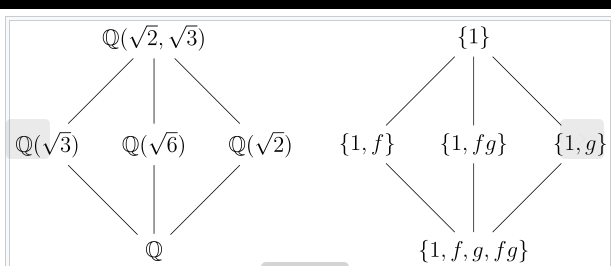
\includegraphics{figures/image_2021-04-17-02-44-48.png}
  \caption{image\_2021-04-17-02-44-48}
  \end{figure}
\end{itemize}

\end{concept}

\begin{solution}

\envlist

Let \(K = {\mathbb{Q}}(\zeta)\). Then \(K\) is the splitting field of
\(f(x) = x^n - 1\), which is irreducible over \({\mathbb{Q}}\), so
\(K/{\mathbb{Q}}\) is normal. We also have \(f'(x) = nx^{n-1}\) and
\(\gcd(f, f') = 1\) since they can not share any roots.

\begin{quote}
Or equivalently, \(f\) splits into distinct linear factors
\(f(x) = \prod_{k\leq n}(x-\zeta^k)\).
\end{quote}

Since it is a Galois extension,
\({\left\lvert {\operatorname{Gal}(K/{\mathbb{Q}})} \right\rvert} = [K: {\mathbb{Q}}] = \phi(n)\)
for the totient function.

We can now define maps
\begin{align*}
\tau_j: K &\to K \\
\zeta &\mapsto \zeta^j 
\end{align*}
and if we restrict to \(j\) such that \(\gcd(n, j) = 1\), this yields
\(\phi(n)\) maps. Noting that if \(\zeta\) is a primitive root, then
\((n, j) = 1\) implies that that \(\zeta^j\) is also a primitive root,
and hence another root of \(\min(\zeta, {\mathbb{Q}})\), and so these
are in fact automorphisms of \(K\) that fix \({\mathbb{Q}}\) and thus
elements of \(\operatorname{Gal}(K/{\mathbb{Q}})\).

So define a map
\begin{align*}
\theta: {\mathbb{Z}}_n^{\times}&\to K \\
[j]_n &\mapsto \tau_j
.\end{align*}

from the \emph{multiplicative} group of units to the Galois group.

The claim is that this is a surjective homomorphism, and since both
groups are the same size, an isomorphism.

\begin{proof}[of surjectivity]

Letting \(\sigma \in K\) be arbitrary, noting that \([K: {\mathbb{Q}}]\)
has a basis \(\left\{{1, \zeta, \zeta^2, \cdots, \zeta^{n-1}}\right\}\),
it suffices to specify \(\sigma(\zeta)\) to fully determine the
automorphism. (Since \(\sigma(\zeta^k) = \sigma(\zeta)^k\).)

In particular, \(\sigma(\zeta)\) satisfies the polynomial \(x^n - 1\),
since \(\sigma(\zeta)^n = \sigma(\zeta^n) = \sigma(1) = 1\), which means
\(\sigma(\zeta)\) is another root of unity and
\(\sigma(\zeta) = \zeta^k\) for some \(1\leq k \leq n\).

Moreover, since \(o(\zeta) = n \in K^{\times}\), we must have
\(o(\zeta^k) = n \in K^{\times}\) as well. Noting that
\(\left\{{\zeta^i}\right\}\) forms a cyclic subgroup
\(H\leq K^{\times}\), then \(o(\zeta^k) = n \iff (n, k) = 1\) (by
general theory of cyclic groups).

Thus \(\theta\) is surjective.

\end{proof}

\begin{proof}[of being a homomorphism]

\begin{align*}
\tau_j \circ \tau_k (\zeta) =\tau_j(\zeta^k) = \zeta^{jk} \implies
\tau_{jk} = \theta(jk) = \tau_j \circ \tau_k
.\end{align*}

\end{proof}

\begin{proof}[of part 2]

We have \(K \cong {\mathbb{Z}}_{20}^{\times}\) and \(\phi(20) = 8\), so
\(K \cong {\mathbb{Z}}_8\), so we have the following subgroups and
corresponding intermediate fields:

\begin{itemize}
\tightlist
\item
  \(0 \sim {\mathbb{Q}}(\zeta_{20})\)
\item
  \({\mathbb{Z}}_2 \sim {\mathbb{Q}}(\omega_1)\)
\item
  \({\mathbb{Z}}_4 \sim {\mathbb{Q}}(\omega_2)\)
\item
  \({\mathbb{Z}}_8 \sim {\mathbb{Q}}\)
\end{itemize}

For some elements \(\omega_i\) which exist by the primitive element
theorem.

\end{proof}

\end{solution}

\hypertarget{spring-2019-2-done}{%
\subsection{\texorpdfstring{Spring 2019 \#2
\(\done\)}{Spring 2019 \#2 \textbackslash done}}\label{spring-2019-2-done}}

Let \(F = {\mathbb{F}}_p\) , where \(p\) is a prime number.

\begin{enumerate}
\def\labelenumi{\alph{enumi}.}
\item
  Show that if \(\pi(x) \in F[x]\) is irreducible of degree \(d\), then
  \(\pi(x)\) divides \(x^{p^d} - x\).
\item
  Show that if \(\pi(x) \in F[x]\) is an irreducible polynomial that
  divides \(x^{p^n} - x\), then \(\deg \pi(x)\) divides \(n\).
\end{enumerate}

\begin{concept}

\envlist

\begin{itemize}
\tightlist
\item
  Go to a field extension.

  \begin{itemize}
  \tightlist
  \item
    Orders of multiplicative groups for finite fields are known.
  \end{itemize}
\item
  \({\mathbb{GF}}(p^n)\) is the splitting field of
  \(x^{p^n} - x \in {\mathbb{F}}_p[x]\).
\item
  \(x^{p^d} - x \bigm|x^{p^n} - x \iff d \bigm|n\)
\item
  \({\mathbb{GF}}(p^d) \leq {\mathbb{GF}}(p^n) \iff d\bigm|n\)
\item
  \(x^{p^n} - x = \prod f_i(x)\) over all irreducible monic \(f_i\) of
  degree \(d\) dividing \(n\).
\end{itemize}

\end{concept}

\begin{solution}

\envlist

\begin{proof}[of a]

We can consider the quotient
\(K = \displaystyle{\frac{{\mathbb{F}}_p[x]}{\left\langle{\pi(x)}\right\rangle}}\),
which since \(\pi(x)\) is irreducible is an extension of
\({\mathbb{F}}_p\) of degree \(d\) and thus a field of size \(p^d\) with
a natural quotient map of rings \(\rho: {\mathbb{F}}_p[x] \to K\).

Since \(K^{\times}\) is a group of size \(p^d-1\), we know that for any
\(y \in K^{\times}\), we have by Lagrange's theorem that the order of
\(y\) divides \(p^d-1\) and so \(y^{p^d} = y\).

So every element in \(K\) is a root of \(q(x) = x^{p^d}-x\).

Since \(\rho\) is a ring morphism, we have

\begin{align*}
\rho(q(x)) = \rho(x^{p^d} - x) &= \rho(x)^{p^d} - \rho(x)
= 0 \in K \\
&\iff q(x) \in \ker \rho \\
&\iff q(x) \in \left\langle{\pi(x)}\right\rangle \\
&\iff \pi(x) \bigm|q(x) = x^{p^d}-x
,\end{align*}
where we've used that ``to contain is to divide'' in the last step.

\end{proof}

\begin{proof}[of b]

\begin{claim}

\(\pi(x)\) divides \(x^{p^n}-x \iff \deg \pi\) divides \(n\).

\end{claim}

\begin{proof}[of claim, $\implies$]

Let \(L \cong {\mathbb{GF}}(p^n)\) be the splitting field of
\(\phi_n(x) \coloneqq x^{p^n}-x\); then since \(\pi \bigm|\phi_n\) by
assumption, \(\pi\) splits in \(L\). Let \(\alpha \in L\) be any root of
\(\pi\); then there is a tower of extensions
\({\mathbb{F}}_p \leq {\mathbb{F}}_p(\alpha) \leq L\).

Then \({\mathbb{F}}_p \leq {\mathbb{F}}_p(\alpha) \leq L\), and so
\begin{align*}
n &= [L: {\mathbb{F}}_p] \\
&= [L: {\mathbb{F}}_p(\alpha)]~[{\mathbb{F}}_p(\alpha): {\mathbb{F}}_p] \\
&= \ell d
,\end{align*}

for some \(\ell \in {\mathbb{Z}}^{\geq 1}\), so \(d\) divides \(n\).

\end{proof}

\begin{proof}[of claim, $\impliedby$]

\(\impliedby\): If \(d\bigm|n\), use the fact (claim) that
\(x^{p^n} - x = \prod f_i(x)\) over all irreducible monic \(f_i\) of
degree \(d\) dividing \(n\). So \(f = f_i\) for some \(i\).

\end{proof}

\end{proof}

\end{solution}

\hypertarget{spring-2019-8-done}{%
\subsection{\texorpdfstring{Spring 2019 \#8
\(\done\)}{Spring 2019 \#8 \textbackslash done}}\label{spring-2019-8-done}}

Let \(\zeta = e^{2\pi i/8}\).

\begin{enumerate}
\def\labelenumi{\alph{enumi}.}
\item
  What is the degree of \({\mathbb{Q}}(\zeta)/{\mathbb{Q}}\)?
\item
  How many quadratic subfields of \({\mathbb{Q}}(\zeta)\) are there?
\item
  What is the degree of \({\mathbb{Q}}(\zeta, \sqrt[4] 2)\) over
  \({\mathbb{Q}}\)?
\end{enumerate}

\begin{concept}

\envlist

\begin{itemize}
\tightlist
\item
  \(\zeta_n \coloneqq e^{2\pi i \over n}\), and \(\zeta_n^k\) is a
  primitive \(n\)th root of unity \(\iff \gcd(n, k) = 1\)

  \begin{itemize}
  \tightlist
  \item
    In general, \(\zeta_n^k\) is a primitive \({n \over \gcd(n, k)}\)th
    root of unity.
  \end{itemize}
\item
  \(\deg \Phi_n(x) = \phi(n)\)
\item
  \(\phi(p^k) = p^k - p^{k-1} = p^{k-1}(p-1)\)

  \begin{itemize}
  \tightlist
  \item
    Proof: for a nontrivial gcd, the possibilities are
    \begin{align*}
    p, 2p, 3p, 4p, \cdots, p^{k-2}p, p^{k-1}p
    .\end{align*}
  \end{itemize}
\item
  \(\operatorname{Gal}({\mathbb{Q}}(\zeta)/{\mathbb{Q}}) \cong {\mathbb{Z}}/(n)^{\times}\)
\end{itemize}

\end{concept}

\begin{solution}

\envlist

Let \(K = {\mathbb{Q}}(\zeta)\).

\begin{proof}[of a]

\envlist

\begin{itemize}
\tightlist
\item
  \(\zeta \coloneqq e^{2\pi i / 8}\) is a primitive \(8\)th root of
  unity
\item
  The minimal polynomial of an \(n\)th root of unity is the \(n\)th
  cyclotomic polynomial \(\Phi_n\)
\item
  The degree of the field extension is the degree of \(\Phi_8\), which
  is
  \begin{align*}
  \phi(8) = \phi(2^3) = 2^{3-1} \cdot (2-1) = 4
  .\end{align*}
\item
  So \([{\mathbb{Q}}(\zeta): {\mathbb{Q}}] = 4\).
\end{itemize}

\end{proof}

\begin{proof}[of b]

\envlist

\begin{itemize}
\tightlist
\item
  \(\operatorname{Gal}({\mathbb{Q}}(\zeta)/{\mathbb{Q}}) \cong {\mathbb{Z}}/(8)^{\times}\cong {\mathbb{Z}}/(4)\)
  by general theory
\item
  \({\mathbb{Z}}/(4)\) has exactly one subgroup of index 2.
\item
  Thus there is exactly \textbf{one} intermediate field of degree 2 (a
  quadratic extension).
\end{itemize}

\end{proof}

\begin{proof}[of c]

\envlist

\begin{itemize}
\item
  Let \(L = {\mathbb{Q}}(\zeta, \sqrt[4] 2)\).
\item
  Note \({\mathbb{Q}}(\zeta) = {\mathbb{Q}}(i, \sqrt 2)\)

  \begin{itemize}
  \tightlist
  \item
    \({\mathbb{Q}}(i, \sqrt{2})\subseteq {\mathbb{Q}}(\zeta)\)

    \begin{itemize}
    \tightlist
    \item
      \(\zeta_8^2 = i\), and \(\zeta_8 = \sqrt{2}^{-1}+ i\sqrt{2}^{-1}\)
      so \(\zeta_8 + \zeta_8 ^{-1}= 2/\sqrt{2} = \sqrt{2}\).
    \end{itemize}
  \item
    \({\mathbb{Q}}(\zeta) \subseteq {\mathbb{Q}}(i, \sqrt{2})\):

    \begin{itemize}
    \tightlist
    \item
      \(\zeta = e^{2\pi i / 8} = \sin(\pi/4) + i\cos(\pi/4) = {\sqrt 2 \over 2}\qty{1+i}\).
    \end{itemize}
  \end{itemize}
\item
  Thus
  \(L = {\mathbb{Q}}(i, \sqrt{2})(\sqrt[4]{2}) = {\mathbb{Q}}(i, \sqrt 2, \sqrt[4] 2) = {\mathbb{Q}}(i, \sqrt[4]{2})\).

  \begin{itemize}
  \tightlist
  \item
    Uses the fact that
    \({\mathbb{Q}}(\sqrt 2) \subseteq {\mathbb{Q}}(\sqrt[4] 2)\) since
    \(\sqrt[4]{2}^2 = \sqrt{2}\)
  \end{itemize}
\item
  Conclude
  \begin{align*}
  [L: {\mathbb{Q}}] = [L: {\mathbb{Q}}(\sqrt[4] 2)] ~[{\mathbb{Q}}(\sqrt[4] 2): {\mathbb{Q}}] = 2 \cdot 4 = 8
  \end{align*}
  using the fact that the minimal polynomial of \(i\) over any subfield
  of \({\mathbb{R}}\) is always \(x^2 + 1\), so
  \(\min_{{\mathbb{Q}}(\sqrt[4] 2)}(i) = x^2 + 1\) which is degree 2.
\end{itemize}

\end{proof}

\end{solution}

\hypertarget{fall-2018-3-done}{%
\subsection{\texorpdfstring{Fall 2018 \#3
\(\done\)}{Fall 2018 \#3 \textbackslash done}}\label{fall-2018-3-done}}

Let \(F \subset K \subset L\) be finite degree field extensions. For
each of the following assertions, give a proof or a counterexample.

\begin{enumerate}
\def\labelenumi{\alph{enumi}.}
\item
  If \(L/F\) is Galois, then so is \(K/F\).
\item
  If \(L/F\) is Galois, then so is \(L/K\).
\item
  If \(K/F\) and \(L/K\) are both Galois, then so is \(L/F\).
\end{enumerate}

\begin{concept}

\envlist

\begin{itemize}
\tightlist
\item
  Every quadratic extension over \({\mathbb{Q}}\) is Galois.
\end{itemize}

\end{concept}

\begin{solution}

Let \(L/K/F\).

\begin{proof}[of a]

\textbf{False}: Take
\(L/K/F = {\mathbb{Q}}(\zeta_2, \sqrt[3] 2) \to {\mathbb{Q}}(\sqrt[3] 2) \to {\mathbb{Q}}\).

Then \(L/F\) is Galois, since it is the splitting field of \(x^3 - 2\)
and \({\mathbb{Q}}\) has characteristic zero.

But \(K/F\) is not Galois, since it is not the splitting field of any
irreducible polynomial.

\end{proof}

\begin{proof}[of b]

\textbf{True}: If \(L/F\) is Galois, then \(L/K\) is normal and
separable:

\begin{itemize}
\item
  \(L/K\) is normal, since if \(\sigma: L \hookrightarrow\overline K\)
  lifts the identity on \(K\) and fixes \(L\), i-t also lifts the
  identity on \(F\) and fixes \(L\) (and \(\overline K = \overline F\)).
\item
  \(L/K\) is separable, since \(F[x] \subseteq K[x]\), and so if
  \(\alpha \in L\) where \(f(x) \coloneqq\min(\alpha, F)\) has no
  repeated factors, then \(f'(x) \coloneqq\min(\alpha, K)\) divides
  \(f\) and thus can not have repeated factors.
\end{itemize}

\end{proof}

\begin{proof}[of c]

\textbf{False}: Use the fact that every quadratic extension is Galois,
and take
\(L/K/F = {\mathbb{Q}}(\sqrt[4] 2) \to {\mathbb{Q}}(\sqrt 2) \to {\mathbb{Q}}\).

Then each successive extension is quadratic (thus Galois) but
\({\mathbb{Q}}(\sqrt[4] 2)\) is not the splitting field of any
polynomial (noting that it does not split \(x^4 - 2\) completely.)

\end{proof}

\end{solution}

\hypertarget{spring-2018-2-done}{%
\subsection{\texorpdfstring{Spring 2018 \#2
\(\done\)}{Spring 2018 \#2 \textbackslash done}}\label{spring-2018-2-done}}

Let \(f(x) = x^4 - 4x^2 + 2 \in {\mathbb{Q}}[x]\).

\begin{enumerate}
\def\labelenumi{\alph{enumi}.}
\item
  Find the splitting field \(K\) of \(f\), and compute
  \([K: {\mathbb{Q}}]\).
\item
  Find the Galois group \(G\) of \(f\), both as an explicit group of
  automorphisms, and as a familiar abstract group to which it is
  isomorphic.
\item
  Exhibit explicitly the correspondence between subgroups of \(G\) and
  intermediate fields between \({\mathbb{Q}}\) and \(k\).
\end{enumerate}

\todo[inline]{Not the nicest proof! Would be better to replace the ad-hoc computations at the end.}

\begin{concept}

\envlist

\begin{itemize}
\tightlist
\item
  Todo
\end{itemize}

\end{concept}

\begin{solution}

\envlist

\begin{proof}[of a]

Note that \(g(x) = x^2 - 4x + 2\) has roots \(\beta = 2 \pm \sqrt{2}\),
and so \(f\) has roots
\begin{align*}
\alpha_1 &= \sqrt{2 + \sqrt 2} \\
\alpha_2 &= \sqrt{2 - \sqrt 2} \\
\alpha_3 &= -\alpha_1 \\
\alpha_4 &= -\alpha_2
.\end{align*}

and splitting field \(K = {\mathbb{Q}}(\left\{{\alpha_i}\right\})\).

\end{proof}

\begin{proof}[of b]

\(K\) is the splitting field of a separable polynomial and thus Galois
over \({\mathbb{Q}}\). Moreover, Since \(f\) is irreducible by
Eisenstein with \(p=2\), the Galois group is a transitive subgroup of
\(S^4\), so the possibilities are:

\begin{itemize}
\tightlist
\item
  \(S_4\)
\item
  \(A_4\)
\item
  \(D_4\)
\item
  \({\mathbb{Z}}/(2) \times{\mathbb{Z}}/(2)\)
\item
  \({\mathbb{Z}}/(4)\)
\end{itemize}

We can note that \(g\) splits over \(L \coloneqq{\mathbb{Q}}(\sqrt 2)\),
an extension of degree 2.

We can now note that \(\min(\alpha, L)\) is given by
\(p(x) = x^2 - (2 + \sqrt 2)\), and so \([K: L] = 2\).

We then have
\begin{align*}
[K: {\mathbb{Q}}] = [K: L] [L : {\mathbb{Q}}] = (2)(2) = 4
.\end{align*}

This
\({\left\lvert {\operatorname{Gal}(K/{\mathbb{Q}})} \right\rvert} = 4\),
which leaves only two possibilities:

\begin{itemize}
\tightlist
\item
  \({\mathbb{Z}}/(2) \times{\mathbb{Z}}/(2)\)
\item
  \({\mathbb{Z}}/(4)\)
\end{itemize}

We can next check orders of elements. Take
\begin{align*}
\sigma &\in \operatorname{Gal}(K/{\mathbb{Q}}) \\
\alpha_1 &\mapsto \alpha_2
.\end{align*}

Computations show that

\begin{itemize}
\tightlist
\item
  \(\alpha_1^2 \alpha_2^2 = 2\), so \(\alpha_1 \alpha_2 = \sqrt 2\)
\item
  \(\alpha_1^2 = 2 + \sqrt 2 \implies \sqrt 2 = \alpha_1^2 - 2\)
\end{itemize}

and thus
\begin{align*}
\sigma^2(\alpha_1) &= \sigma(\alpha_2) \\
&= \sigma\left(\frac{\sqrt 2}{\alpha_1}\right) \\
&= \frac{\sigma(\sqrt 2)}{\sigma(\alpha_1)} \\
&= \frac{\sigma(\alpha_1^2 - 2)}{\alpha_2} \\
&= \frac{\alpha_2^2 - 2}{\alpha_2} \\
&= \alpha_2 -2\alpha_2^{-1}\\
&= \alpha_2 - \frac{2\alpha_1}{\sqrt 2} \\
&= \alpha_2 -\alpha_1 \sqrt 2 \\
&\neq \alpha_1
,\end{align*}

and so the order of \(\sigma\) is strictly greater than 2, and thus 4,
and thus
\(\operatorname{Gal}(K/{\mathbb{Q}}) = \left\{{\sigma^k {~\mathrel{\Big|}~}1\leq k \leq 4}\right\} \cong {\mathbb{Z}}/(4)\).

\end{proof}

\begin{proof}[of c]

?? The subgroup of index 2 \(\left\langle{\sigma^2}\right\rangle\)
corresponds to the field extension \(Q(\sqrt 2) / {\mathbb{Q}}\).

\end{proof}

\todo[inline]{Finish (c)}

\end{solution}

\hypertarget{spring-2018-3-done}{%
\subsection{\texorpdfstring{Spring 2018 \#3
\(\done\)}{Spring 2018 \#3 \textbackslash done}}\label{spring-2018-3-done}}

Let \(K\) be a Galois extension of \({\mathbb{Q}}\) with Galois group
\(G\), and let \(E_1 , E_2\) be intermediate fields of \(K\) which are
the splitting fields of irreducible \(f_i (x) \in {\mathbb{Q}}[x]\).

Let \(E = E_1 E_2 \subset K\).

Let \(H_i = \operatorname{Gal}(K/E_i)\) and
\(H = \operatorname{Gal}(K/E)\).

\begin{enumerate}
\def\labelenumi{\alph{enumi}.}
\item
  Show that \(H = H_1 \cap H_2\).
\item
  Show that \(H_1 H_2\) is a subgroup of \(G\).
\item
  Show that
  \begin{align*}
  \operatorname{Gal}(K/(E_1 \cap E_2 )) = H_1 H_2
  .\end{align*}
\end{enumerate}

\begin{concept}

\envlist

\begin{itemize}
\tightlist
\item
  The Galois correspondence:

  \begin{itemize}
  \tightlist
  \item
    \(H_1 \cap H_2 \rightleftharpoons E_1 E_2\),
  \item
    \(H_1 H_2 \rightleftharpoons E_1 \cap E_2\).
  \end{itemize}
\end{itemize}

\end{concept}

\begin{solution}

\envlist

\begin{proof}[of a]

By the Galois correspondence, it suffices to show that the fixed field
of \(H_1 \cap H_2\) is \(E_1 E_2\).

Let \(\sigma \in H_1 \cap H_2\); then
\(\sigma \in {\operatorname{Aut}}(K)\) fixes both \(E_1\) and \(E_2\).

\begin{quote}
Not sure if this works -- compositum is not literally product..?
\end{quote}

Writing \(x \in E_1E_2\) as \(x=e_1 e_2\), we have
\begin{align*}
\sigma(x) = \sigma(e_1 e_2) = \sigma(e_1) \sigma(e_2) = e_1 e_2  =x,
\end{align*}

so \(\sigma\) fixes \(E_1 E_2\).

\end{proof}

\begin{proof}[of b]

That \(H_1 H_2 \subseteq G\) is clear, since if
\(\sigma = \tau_1 \tau_2 \in H_1 H_2\), then each \(\tau_i\) is an
automorphism of \(K\) that fixes \(E_i \supseteq {\mathbb{Q}}\), so each
\(\tau_i\) fixes \({\mathbb{Q}}\) and thus \(\sigma\) fixes
\({\mathbb{Q}}\).

\begin{claim}

All elements in this subset commute.

\end{claim}

\begin{proof}[of claim]

\envlist

\begin{itemize}
\item
  Let \(\sigma = \sigma_1 \sigma_2 \in H_1 H_2\).
\item
  Note that \(\sigma_1(e) = e\) for all \(e\in E_1\) by definition,
  since \(H_1\) fixes \(E_1\), and \(\sigma_2(e) \in E_1\) (?).
\item
  Then
  \begin{align*}
  \sigma_1(e) = e \quad \forall e \in E_1 \implies \sigma_1(\sigma_2(e)) = \sigma_2(e) 
  \end{align*}
  and substituting \(e = \sigma_1(e)\) on the RHS yields
  \begin{align*}
  \sigma_1 \sigma_2(e) = \sigma_2 \sigma_1(e)
  ,\end{align*}
  where a similar proof holds for \(e\in E_2\) and thus for arbitrary
  \(x\in E_1 E_2\).
\end{itemize}

\end{proof}

\end{proof}

\begin{proof}[of c]

By the Galois correspondence, the subgroup \(H_1H_2 \leq G\) will
correspond to an intermediate field \(E\) such that \(K/E/{\mathbb{Q}}\)
and \(E\) is the fixed field of \(H_1 H_2\).

But if \(\sigma \in H_1 H_2\), then \(\sigma = \tau_1 \tau_2\) where
\(\tau_i\) is an automorphism of \(K\) that fixes \(E_i\), and so
\begin{align*}
\sigma(x) = x \iff \tau_1\tau_2(x) = x
&\iff \tau_2(x) = x 
\\
&~\&~ 
\\
\tau_1(x) = x &\iff x \in E_1 \cap E_2
.\end{align*}
.

\end{proof}

\end{solution}

\hypertarget{spring-2020-4-work}{%
\subsection{\texorpdfstring{Spring 2020 \#4
\(\work\)}{Spring 2020 \#4 \textbackslash work}}\label{spring-2020-4-work}}

Let \(f(x) = x^4-2 \in {\mathbb{Q}}[x]\).

\begin{enumerate}
\def\labelenumi{\alph{enumi}.}
\item
  Define what it means for a finite extension field \(E\) of a field
  \(F\) to be a Galois extension.
\item
  Determine the Galois group \(\operatorname{Gal}(E/{\mathbb{Q}})\) for
  the polynomial \(f(x)\), and justify your answer carefully.
\item
  Exhibit a subfield \(K\) in \((b)\) such that
  \({\mathbb{Q}}\leq K \leq E\) with \(K\) not a Galois extension over
  \({\mathbb{Q}}\). Explain.
\end{enumerate}

\hypertarget{spring-2020-3-work}{%
\subsection{\texorpdfstring{Spring 2020 \#3
\(\work\)}{Spring 2020 \#3 \textbackslash work}}\label{spring-2020-3-work}}

Let \(E\) be an extension field of \(F\) and \(\alpha\in E\) be
algebraic of odd degree over \(F\).

\begin{enumerate}
\def\labelenumi{\alph{enumi}.}
\item
  Show that \(F(\alpha) = F(\alpha^2)\).
\item
  Prove that \(\alpha^{2020}\) is algebraic of odd degree over \(F\).
\end{enumerate}

\hypertarget{fall-2017-4-work}{%
\subsection{\texorpdfstring{Fall 2017 \#4
\(\work\)}{Fall 2017 \#4 \textbackslash work}}\label{fall-2017-4-work}}

\begin{enumerate}
\def\labelenumi{\alph{enumi}.}
\item
  Let \(f (x)\) be an irreducible polynomial of degree 4 in
  \({\mathbb{Q}}[x]\) whose splitting field \(K\) over \({\mathbb{Q}}\)
  has Galois group \(G = S_4\).

  Let \(\theta\) be a root of \(f(x)\). Prove that
  \({\mathbb{Q}}[\theta]\) is an extension of \({\mathbb{Q}}\) of degree
  4 and that there are no intermediate fields between \({\mathbb{Q}}\)
  and \({\mathbb{Q}}[\theta]\).
\item
  Prove that if \(K\) is a Galois extension of \({\mathbb{Q}}\) of
  degree 4, then there is an intermediate subfield between \(K\) and
  \({\mathbb{Q}}\).
\end{enumerate}

\hypertarget{fall-2017-3-work}{%
\subsection{\texorpdfstring{Fall 2017 \#3
\(\work\)}{Fall 2017 \#3 \textbackslash work}}\label{fall-2017-3-work}}

Let \(F\) be a field. Let \(f(x)\) be an irreducible polynomial in
\(F[x]\) of degree \(n\) and let \(g(x)\) be any polynomial in \(F[x]\).
Let \(p(x)\) be an irreducible factor (of degree \(m\)) of the
polynomial \(f(g(x))\).

Prove that \(n\) divides \(m\). Use this to prove that if \(r\) is an
integer which is not a perfect square, and \(n\) is a positive integer
then every irreducible factor of \(x^{2n} - r\) over \({\mathbb{Q}}[x]\)
has even degree.

\hypertarget{spring-2017-7-work}{%
\subsection{\texorpdfstring{Spring 2017 \#7
\(\work\)}{Spring 2017 \#7 \textbackslash work}}\label{spring-2017-7-work}}

Let \(F\) be a field and let \(f(x) \in F[x]\).

\begin{enumerate}
\def\labelenumi{\alph{enumi}.}
\item
  Define what a splitting field of \(f(x)\) over \(F\) is.
\item
  Let \(F\) now be a finite field with \(q\) elements. Let \(E/F\) be a
  finite extension of degree \(n>0\). Exhibit an explicit polynomial
  \(g(x) \in F[x]\) such that \(E/F\) is a splitting field of \(g(x)\)
  over \(F\). Fully justify your answer.
\item
  Show that the extension \(E/F\) in (b) is a Galois extension.
\end{enumerate}

\hypertarget{spring-2017-8-work}{%
\subsection{\texorpdfstring{Spring 2017 \#8
\(\work\)}{Spring 2017 \#8 \textbackslash work}}\label{spring-2017-8-work}}

\begin{enumerate}
\def\labelenumi{\alph{enumi}.}
\item
  Let \(K\) denote the splitting field of \(x^5 - 2\) over
  \({\mathbb{Q}}\). Show that the Galois group of \(K/{\mathbb{Q}}\) is
  isomorphic to the group of invertible matrices
  \begin{align*}
  \left(\begin{array}{ll}
  a & b \\
  0 & 1
  \end{array}\right) 
  {\quad \operatorname{where} \quad} a\in {\mathbb{F}}_5^{\times}\text{ and } b\in {\mathbb{F}}_5
  .\end{align*}
\item
  Determine all intermediate fields between \(K\) and \({\mathbb{Q}}\)
  which are Galois over \({\mathbb{Q}}\).
\end{enumerate}

\hypertarget{fall-2016-4-work}{%
\subsection{\texorpdfstring{Fall 2016 \#4
\(\work\)}{Fall 2016 \#4 \textbackslash work}}\label{fall-2016-4-work}}

Set \(f(x) = x^3 - 5 \in {\mathbb{Q}}[x]\).

\begin{enumerate}
\def\labelenumi{\alph{enumi}.}
\item
  Find the splitting field \(K\) of \(f(x)\) over \({\mathbb{Q}}\).
\item
  Find the Galois group \(G\) of \(K\) over \({\mathbb{Q}}\).
\item
  Exhibit explicitly the correspondence between subgroups of \(G\) and
  intermediate fields between \({\mathbb{Q}}\) and \(K\).
\end{enumerate}

\hypertarget{spring-2016-2-work}{%
\subsection{\texorpdfstring{Spring 2016 \#2
\(\work\)}{Spring 2016 \#2 \textbackslash work}}\label{spring-2016-2-work}}

Let \(K = {\mathbb{Q}}[\sqrt 2 + \sqrt 5]\).

\begin{enumerate}
\def\labelenumi{\alph{enumi}.}
\item
  Find \([K: {\mathbb{Q}}]\).
\item
  Show that \(K/{\mathbb{Q}}\) is Galois, and find the Galois group
  \(G\) of \(K/{\mathbb{Q}}\).
\item
  Exhibit explicitly the correspondence between subgroups of \(G\) and
  intermediate fields between \({\mathbb{Q}}\) and \(K\).
\end{enumerate}

\hypertarget{spring-2016-6-work}{%
\subsection{\texorpdfstring{Spring 2016 \#6
\(\work\)}{Spring 2016 \#6 \textbackslash work}}\label{spring-2016-6-work}}

Let \(K\) be a Galois extension of a field \(F\) with \([K: F] = 2015\).
Prove that \(K\) is an extension by radicals of the field \(F\).

\hypertarget{fall-2015-5-work}{%
\subsection{\texorpdfstring{Fall 2015 \#5
\(\work\)}{Fall 2015 \#5 \textbackslash work}}\label{fall-2015-5-work}}

Let \(u = \sqrt{2 + \sqrt{2}}\), \(v = \sqrt{2 - \sqrt{2}}\), and
\(E = {\mathbb{Q}}(u)\).

\begin{enumerate}
\def\labelenumi{\alph{enumi}.}
\item
  Find (with justification) the minimal polynomial \(f(x)\) of \(u\)
  over \({\mathbb{Q}}\).
\item
  Show \(v\in E\), and show that \(E\) is a splitting field of \(f(x)\)
  over \({\mathbb{Q}}\).
\item
  Determine the Galois group of \(E\) over \({\mathbb{Q}}\) and
  determine all of the intermediate fields \(F\) such that
  \({\mathbb{Q}}\subset F \subset E\).
\end{enumerate}

\hypertarget{fall-2015-6-work}{%
\subsection{\texorpdfstring{Fall 2015 \#6
\(\work\)}{Fall 2015 \#6 \textbackslash work}}\label{fall-2015-6-work}}

\begin{enumerate}
\def\labelenumi{\alph{enumi}.}
\item
  Let \(G\) be a finite group. Show that there exists a field extension
  \(K/F\) with \(\operatorname{Gal}(K/F) = G\).

  \begin{quote}
  You may assume that for any natural number \(n\) there is a field
  extension with Galois group \(S_n\).
  \end{quote}
\item
  Let \(K\) be a Galois extension of \(F\) with
  \({\left\lvert {\operatorname{Gal}(K/F)} \right\rvert} = 12\). Prove
  that there exists an intermediate field \(E\) of \(K/F\) with
  \([E: F] = 3\).
\item
  With \(K/F\) as in (b), does an intermediate field \(L\) necessarily
  exist satisfying \([L: F] = 2\)? Give a proof or counterexample.
\end{enumerate}

\hypertarget{spring-2015-2-work}{%
\subsection{\texorpdfstring{Spring 2015 \#2
\(\work\)}{Spring 2015 \#2 \textbackslash work}}\label{spring-2015-2-work}}

Let \({\mathbb{F}}\) be a finite field.

\begin{enumerate}
\def\labelenumi{\alph{enumi}.}
\item
  Give (with proof) the decomposition of the additive group
  \(({\mathbb{F}}, +)\) into a direct sum of cyclic groups.
\item
  The \emph{exponent} of a finite group is the least common multiple of
  the orders of its elements. Prove that a finite abelian group has an
  element of order equal to its exponent.
\item
  Prove that the multiplicative group \(({\mathbb{F}}^{\times}, \cdot)\)
  is cyclic.
\end{enumerate}

\hypertarget{spring-2015-5-work}{%
\subsection{\texorpdfstring{Spring 2015 \#5
\(\work\)}{Spring 2015 \#5 \textbackslash work}}\label{spring-2015-5-work}}

Let \(f(x) = x^4 - 5 \in {\mathbb{Q}}[x]\).

\begin{enumerate}
\def\labelenumi{\alph{enumi}.}
\item
  Compute the Galois group of \(f\) over \({\mathbb{Q}}\).
\item
  Compute the Galois group of \(f\) over \({\mathbb{Q}}(\sqrt{5})\).
\end{enumerate}

\hypertarget{fall-2014-1-work}{%
\subsection{\texorpdfstring{Fall 2014 \#1
\(\work\)}{Fall 2014 \#1 \textbackslash work}}\label{fall-2014-1-work}}

Let \(f\in {\mathbb{Q}}[x]\) be an irreducible polynomial and \(L\) a
finite Galois extension of \({\mathbb{Q}}\). Let
\(f(x) = g_1(x)g_2(x)\cdots g_r(x)\) be a factorization of \(f\) into
irreducibles in \(L[x]\).

\begin{enumerate}
\def\labelenumi{\alph{enumi}.}
\item
  Prove that each of the factors \(g_i(x)\) has the same degree.
\item
  Give an example showing that if \(L\) is not Galois over
  \({\mathbb{Q}}\), the conclusion of part (a) need not hold.
\end{enumerate}

\hypertarget{fall-2014-3-work}{%
\subsection{\texorpdfstring{Fall 2014 \#3
\(\work\)}{Fall 2014 \#3 \textbackslash work}}\label{fall-2014-3-work}}

Consider the polynomial \(f(x) = x^4 - 7 \in {\mathbb{Q}}[x]\) and let
\(E/{\mathbb{Q}}\) be the splitting field of \(f\).

\begin{enumerate}
\def\labelenumi{\alph{enumi}.}
\item
  What is the structure of the Galois group of \(E/{\mathbb{Q}}\)?
\item
  Give an explicit description of all of the intermediate subfields
  \({\mathbb{Q}}\subset K \subset E\) in the form
  \(K = {\mathbb{Q}}(\alpha), {\mathbb{Q}}(\alpha, \beta), \cdots\)
  where \(\alpha, \beta\), etc are complex numbers. Describe the
  corresponding subgroups of the Galois group.
\end{enumerate}

\hypertarget{spring-2014-3-work}{%
\subsection{\texorpdfstring{Spring 2014 \#3
\(\work\)}{Spring 2014 \#3 \textbackslash work}}\label{spring-2014-3-work}}

Let \(F\subset C\) be a field extension with \(C\) algebraically closed.

\begin{enumerate}
\def\labelenumi{\alph{enumi}.}
\item
  Prove that the intermediate field \(C_{\text{alg}} \subset C\)
  consisting of elements algebraic over \(F\) is algebraically closed.
\item
  Prove that if \(F\to E\) is an algebraic extension, there exists a
  homomorphism \(E\to C\) that is the identity on \(F\).
\end{enumerate}

\hypertarget{spring-2014-4-work}{%
\subsection{\texorpdfstring{Spring 2014 \#4
\(\work\)}{Spring 2014 \#4 \textbackslash work}}\label{spring-2014-4-work}}

Let \(E\subset {\mathbb{C}}\) denote the splitting field over
\({\mathbb{Q}}\) of the polynomial \(x^3 - 11\).

\begin{enumerate}
\def\labelenumi{\alph{enumi}.}
\item
  Prove that if \(n\) is a squarefree positive integer, then
  \(\sqrt{n}\not\in E\).

  \begin{quote}
  Hint: you can describe all quadratic extensions of \({\mathbb{Q}}\)
  contained in \(E\).
  \end{quote}
\item
  Find the Galois group of \((x^3 - 11)(x^2 - 2)\) over
  \({\mathbb{Q}}\).
\item
  Prove that the minimal polynomial of \(11^{1/3} + 2^{1/2}\) over
  \({\mathbb{Q}}\) has degree 6.
\end{enumerate}

\hypertarget{fall-2013-5-work}{%
\subsection{\texorpdfstring{Fall 2013 \#5
\(\work\)}{Fall 2013 \#5 \textbackslash work}}\label{fall-2013-5-work}}

Let \(L/K\) be a finite extension of fields.

\begin{enumerate}
\def\labelenumi{\alph{enumi}.}
\item
  Define what it means for \(L/K\) to be \emph{separable}.
\item
  Show that if \(K\) is a finite field, then \(L/K\) is always
  separable.
\item
  Give an example of a finite extension \(L/K\) that is not separable.
\end{enumerate}

\hypertarget{fall-2013-6-work}{%
\subsection{\texorpdfstring{Fall 2013 \#6
\(\work\)}{Fall 2013 \#6 \textbackslash work}}\label{fall-2013-6-work}}

Let \(K\) be the splitting field of \(x^4-2\) over \({\mathbb{Q}}\) and
set \(G = \operatorname{Gal}(K/{\mathbb{Q}})\).

\begin{enumerate}
\def\labelenumi{\alph{enumi}.}
\item
  Show that \(K/{\mathbb{Q}}\) contains both \({\mathbb{Q}}(i)\) and
  \({\mathbb{Q}}(\sqrt[4]{2})\) and has degree 8 over \({\mathbb{Q}}\)/
\item
  Let \(N = \operatorname{Gal}(K/{\mathbb{Q}}(i))\) and
  \(H = \operatorname{Gal}(K/{\mathbb{Q}}(\sqrt[4]{2}))\). Show that
  \(N\) is normal in \(G\) and \(NH = G\).

  \begin{quote}
  Hint: what field is fixed by \(NH\)?
  \end{quote}
\item
  Show that \(\operatorname{Gal}(K/{\mathbb{Q}})\) is generated by
  elements \(\sigma, \tau\), of orders 4 and 2 respectively, with
  \(\tau \sigma\tau^{-1}= \sigma^{-1}\).

  \begin{quote}
  Equivalently, show it is the dihedral group of order 8.
  \end{quote}
\item
  How many distinct quartic subfields of \(K\) are there? Justify your
  answer.
\end{enumerate}

\hypertarget{spring-2013-7-work}{%
\subsection{\texorpdfstring{Spring 2013 \#7
\(\work\)}{Spring 2013 \#7 \textbackslash work}}\label{spring-2013-7-work}}

Let \(f(x) = g(x) h(x) \in {\mathbb{Q}}[x]\) and \(E,B,C/{\mathbb{Q}}\)
be the splitting fields of \(f,g,h\) respectively.

\begin{enumerate}
\def\labelenumi{\alph{enumi}.}
\item
  Prove that \(\operatorname{Gal}(E/B)\) and \(\operatorname{Gal}(E/C)\)
  are normal subgroups of \(\operatorname{Gal}(E/{\mathbb{Q}})\).
\item
  Prove that
  \(\operatorname{Gal}(E/B) \cap\operatorname{Gal}(E/C) = \left\{{1}\right\}\).
\item
  If \(B\cap C = {\mathbb{Q}}\), show that
  \(\operatorname{Gal}(E/B) \operatorname{Gal}(E/C) = \operatorname{Gal}(E/{\mathbb{Q}})\).
\item
  Under the hypothesis of (c), show that
  \(\operatorname{Gal}(E/{\mathbb{Q}}) \cong \operatorname{Gal}(E/B) \times \operatorname{Gal}(E/C)\).
\item
  Use (d) to describe
  \(\operatorname{Gal}({\mathbb{Q}}[\alpha]/{\mathbb{Q}})\) where
  \(\alpha = \sqrt 2 + \sqrt 3\).
\end{enumerate}

\hypertarget{spring-2013-8-work}{%
\subsection{\texorpdfstring{Spring 2013 \#8
\(\work\)}{Spring 2013 \#8 \textbackslash work}}\label{spring-2013-8-work}}

Let \(F\) be the field with 2 elements and \(K\) a splitting field of
\(f(x) = x^6 + x^3 + 1\) over \(F\). You may assume that \(f\) is
irreducible over \(F\).

\begin{enumerate}
\def\labelenumi{\alph{enumi}.}
\item
  Show that if \(r\) is a root of \(f\) in \(K\), then \(r^9 = 1\) but
  \(r^3\neq 1\).
\item
  Find \(\operatorname{Gal}(K/F)\) and express each intermediate field
  between \(F\) and \(K\) as \(F(\beta)\) for an appropriate
  \(\beta \in K\).
\end{enumerate}

\hypertarget{fall-2012-3-work}{%
\subsection{\texorpdfstring{Fall 2012 \#3
\(\work\)}{Fall 2012 \#3 \textbackslash work}}\label{fall-2012-3-work}}

Let \(f(x) \in {\mathbb{Q}}[x]\) be an irreducible polynomial of degree
5. Assume that \(f\) has all but two roots in \({\mathbb{R}}\). Compute
the Galois group of \(f(x)\) over \({\mathbb{Q}}\) and justify your
answer.

\hypertarget{fall-2012-4-work}{%
\subsection{\texorpdfstring{Fall 2012 \#4
\(\work\)}{Fall 2012 \#4 \textbackslash work}}\label{fall-2012-4-work}}

Let \(f(x) \in {\mathbb{Q}}[x]\) be a polynomial and \(K\) be a
splitting field of \(f\) over \({\mathbb{Q}}\). Assume that
\([K:{\mathbb{Q}}] = 1225\) and show that \(f(x)\) is solvable by
radicals.

\hypertarget{spring-2012-1-work}{%
\subsection{\texorpdfstring{Spring 2012 \#1
\(\work\)}{Spring 2012 \#1 \textbackslash work}}\label{spring-2012-1-work}}

Suppose that \(F\subset E\) are fields such that \(E/F\) is Galois and
\({\left\lvert {\operatorname{Gal}(E/F)} \right\rvert} = 14\).

\begin{enumerate}
\def\labelenumi{\alph{enumi}.}
\item
  Show that there exists a unique intermediate field \(K\) with
  \(F\subset K \subset E\) such that \([K: F] = 2\).
\item
  Assume that there are at least two distinct intermediate subfields
  \(F \subset L_1, L_2 \subset E\) with \([L_i: F]= 7\). Prove that
  \(\operatorname{Gal}(E/F)\) is nonabelian.
\end{enumerate}

\hypertarget{spring-2012-4-work}{%
\subsection{\texorpdfstring{Spring 2012 \#4
\(\work\)}{Spring 2012 \#4 \textbackslash work}}\label{spring-2012-4-work}}

Let \(f(x) = x^7 - 3\in {\mathbb{Q}}[x]\) and \(E/{\mathbb{Q}}\) be a
splitting field of \(f\) with \(\alpha \in E\) a root of \(f\).

\begin{enumerate}
\def\labelenumi{\alph{enumi}.}
\item
  Show that \(E\) contains a primitive 7th root of unity.
\item
  Show that \(E\neq {\mathbb{Q}}(\alpha)\).
\end{enumerate}

\hypertarget{fall-2019-midterm-6-work}{%
\subsection{\texorpdfstring{Fall 2019 Midterm \#6
\(\work\)}{Fall 2019 Midterm \#6 \textbackslash work}}\label{fall-2019-midterm-6-work}}

Compute the Galois group of
\(f(x) = x^3-3x -3\in {\mathbb{Q}}[x]/{\mathbb{Q}}\).

\hypertarget{fall-2019-midterm-7-work}{%
\subsection{\texorpdfstring{Fall 2019 Midterm \#7
\(\work\)}{Fall 2019 Midterm \#7 \textbackslash work}}\label{fall-2019-midterm-7-work}}

Show that a field \(k\) of characteristic \(p\neq 0\) is perfect
\(\iff\) for every \(x\in k\) there exists a \(y\in k\) such that
\(y^p=x\).

\hypertarget{fall-2019-midterm-8-work}{%
\subsection{\texorpdfstring{Fall 2019 Midterm \#8
\(\work\)}{Fall 2019 Midterm \#8 \textbackslash work}}\label{fall-2019-midterm-8-work}}

Let \(k\) be a field of characteristic \(p\neq 0\) and \(f\in k[x]\)
irreducible. Show that \(f(x) = g(x^{p^d})\) where \(g(x) \in k[x]\) is
irreducible and separable.

Conclude that every root of \(f\) has the same multiplicity \(p^d\) in
the splitting field of \(f\) over \(k\).

\hypertarget{fall-2019-midterm-9-work}{%
\subsection{\texorpdfstring{Fall 2019 Midterm \#9
\(\work\)}{Fall 2019 Midterm \#9 \textbackslash work}}\label{fall-2019-midterm-9-work}}

Let \(n\geq 3\) and \(\zeta_n\) be a primitive \(n\)th root of unity.
Show that
\([{\mathbb{Q}}(\zeta_n + \zeta_n^{-1}): {\mathbb{Q}}] = \phi(n)/2\) for
\(\phi\) the totient function. 10.

Let \(L/K\) be a finite normal extension.

\begin{enumerate}
\def\labelenumi{\alph{enumi}.}
\item
  Show that if \(L/K\) is cyclic and \(E/K\) is normal with \(L/E/K\)
  then \(L/E\) and \(E/K\) are cyclic.
\item
  Show that if \(L/K\) is cyclic then there exists exactly one extension
  \(E/K\) of degree \(n\) with \(L/E/K\) for each divisor \(n\) of
  \([L:K]\).
\end{enumerate}

\hypertarget{spring-2021-4-work}{%
\subsection{\texorpdfstring{Spring 2021 \#4
\(\work\)}{Spring 2021 \#4 \textbackslash work}}\label{spring-2021-4-work}}

Define
\begin{align*}
f(x) \coloneqq x^4 + 4x^2 + 64 \in {\mathbb{Q}}[x]
.\end{align*}

\begin{enumerate}
\def\labelenumi{\alph{enumi}.}
\item
  Find the splitting field \(K\) of \(f\) over \({\mathbb{Q}}\).
\item
  Find the Galois group \(G\) of \(f\).
\item
  Exhibit explicitly the correspondence between subgroups of \(G\) and
  intermediate fields between \({\mathbb{Q}}\) and \(K\).
\end{enumerate}

\hypertarget{spring-2021-7-done}{%
\subsection{\texorpdfstring{Spring 2021 \#7
\(\done\)}{Spring 2021 \#7 \textbackslash done}}\label{spring-2021-7-done}}

Let \(p\) be a prime number and let \(F\) be a field of characteristic
\(p\). Show that if \(a\in F\) is not a \(p\)th power in \(F\), then
\(x^p-a \in F[x]\) is irreducible.

\begin{strategy}

\envlist

\begin{itemize}
\tightlist
\item
  By contrapositive, show that
  \(f(x) \coloneqq x^p-a \in {\mathbb{F}}[x]\) reducible \(\implies a\)
  is a \(p\)th power in \({\mathbb{F}}\).
\item
  Eventually show \(a^\ell = b^p\) for some \(\ell\in {\mathbb{N}}\) and
  some \(b\in {\mathbb{F}}\), then \(\gcd(\ell, p) = 1\) forces \(b=a\)
  and \(\ell=p\).
\item
  Use the fact that the constant term of any \(g\in {\mathbb{F}}[x]\) is
  actually in \({\mathbb{F}}\).
\end{itemize}

\end{strategy}

\begin{concept}

\envlist

\begin{itemize}
\tightlist
\item
  Reducible: \(f\in {\mathbb{F}}[x]\) is reducible iff there exists
  \(g, h\in {\mathbb{F}}[x]\) nonconstant with \(f = g h\).

  \begin{itemize}
  \tightlist
  \item
    Importantly, this factorization needs to happen in
    \({\mathbb{F}}[x]\), since we can \emph{always} find such
    factorizations in the splitting field \(\operatorname{SF}(f)[x]\).
  \end{itemize}
\item
  Bezout's identity: \(\gcd(p, q) = d \implies\) there exist
  \(s,t\in {\mathbb{Z}}\) such that
  \begin{align*}
  sp + tq = d
  .\end{align*}
\end{itemize}

\end{concept}

\begin{solution}

\envlist

\begin{itemize}
\item
  WTS: \(f(x) \coloneqq x^p - a\in {\mathbb{F}}[x]\) reducible
  \(\implies f\) has a root in the \emph{base field} \({\mathbb{F}}\).
\item
  Write \(f(x) = g(x) h(x)\) and factor
  \(f(x) = \prod_{i=1}^p (x- r_i) \in \operatorname{SF}(f)[x]\) where
  the \(r_i\) are not necessarily distinct roots.
\item
  WLOG, \(g(x) = \prod_{i=1}^\ell (x-r_i)\) for some
  \(1\leq \ell \leq p-1\), i.e.~rearrange the factors so that \(g\) is
  the first \(\ell\) of them.

  \begin{itemize}
  \tightlist
  \item
    \(\ell \neq 1, p\) since \(f\) is reducible, making \(g, h\)
    nonconstant.
  \end{itemize}
\item
  Set \(R_\ell \coloneqq\prod_{i=1}^\ell r_i\), which is the constant
  term in \(g\), so \(R_\ell \in {\mathbb{F}}\) since
  \(g\in {\mathbb{F}}[x]\).
\item
  Each \(r_i\) is a root of \(f\), so \(r_i^p - a = 0\) for all \(i\),
  so \(r_i^p = a\).
\item
  Trick: what is the \(p\)th power of \(R_\ell\)?
  \begin{align*}
  R_\ell^p 
  &\coloneqq\qty{ \prod_{i=1}^\ell}^p \\
  &= \prod_{i=1}^\ell r_i^p \\
  &= \prod_{i=1}^\ell a \\
  &= a^\ell
  ,\end{align*}
  so \(R_\ell^p = a^\ell\).
\item
  Use Bezout: \(\gcd(\ell, p) = 1\) since \(p\) is prime, so write
  \(tp + s\ell = 1\) for some \(t,s\in {\mathbb{Z}}\)
\item
  Use this to build a root of \(f\) that's in \({\mathbb{F}}\): write
  \begin{align*}
  a &= a^1\\
  &= a^{tp + s\ell} \\
  &= a^{tp} a^{s\ell} \\
  &=a^{tp} (a^\ell)^s\\
  &= a^{tp} (R_\ell^p)^s \\
  &= (a^t R_\ell^s)^p \\
  &\coloneqq\beta^p
  ,\end{align*}
  so \(a = \beta^p\).

  \begin{itemize}
  \tightlist
  \item
    Check \(\beta\in {\mathbb{F}}\): use that
    \(R_\ell \in {\mathbb{F}}\) since it was a constant term of a
    polynomial in \({\mathbb{F}}[x]\), \(a\in {\mathbb{F}}\) by
    assumption, and fields are closed under taking powers and products.
  \end{itemize}
\end{itemize}

\end{solution}

\hypertarget{fall-2020-3-work}{%
\subsection{\texorpdfstring{Fall 2020 \#3
\(\work\)}{Fall 2020 \#3 \textbackslash work}}\label{fall-2020-3-work}}

\begin{enumerate}
\def\labelenumi{\alph{enumi}.}
\item
  Define what it means for a finite extension of fields \(E\) over \(F\)
  to be a \emph{Galois} extension.
\item
  Determine the Galois group of \(f(x) = x^3 - 7\) over
  \({\mathbb{Q}}\), and justify your answer carefully.
\item
  Find all subfields of the splitting field of \(f(x)\) over
  \({\mathbb{Q}}\).
\end{enumerate}

\hypertarget{fall-2020-4-work}{%
\subsection{\texorpdfstring{Fall 2020 \#4
\(\work\)}{Fall 2020 \#4 \textbackslash work}}\label{fall-2020-4-work}}

Let \(K\) be a Galois extension of \(F\), and let
\(F \subset E \subset K\) be inclusions of fields. Let
\(G \coloneqq\operatorname{Gal}(K/F)\) and
\(H \coloneqq\operatorname{Gal}(K/E)\), and suppose \(H\) contains
\(N_G(P)\), where \(P\) is a Sylow \(p\)-subgroup of \(G\) for \(p\) a
prime. Prove that \([E: F] \equiv 1 \pmod p\).

\hypertarget{modules}{%
\section{Modules}\label{modules}}

\hypertarget{general-questions}{%
\subsection{General Questions}\label{general-questions}}

\hypertarget{fall-2018-6-done}{%
\subsubsection{\texorpdfstring{Fall 2018 \#6
\(\done\)}{Fall 2018 \#6 \textbackslash done}}\label{fall-2018-6-done}}

Let \(R\) be a commutative ring, and let \(M\) be an
\(R{\hbox{-}}\)module. An \(R{\hbox{-}}\)submodule \(N\) of \(M\) is
maximal if there is no \(R{\hbox{-}}\)module \(P\) with
\(N \subsetneq P \subsetneq M\).

\begin{enumerate}
\def\labelenumi{\alph{enumi}.}
\item
  Show that an \(R{\hbox{-}}\)submodule \(N\) of \(M\) is maximal
  \(\iff M /N\) is a simple \(R{\hbox{-}}\)module: i.e., \(M /N\) is
  nonzero and has no proper, nonzero \(R{\hbox{-}}\)submodules.
\item
  Let \(M\) be a \({\mathbb{Z}}{\hbox{-}}\)module. Show that a
  \({\mathbb{Z}}{\hbox{-}}\)submodule \(N\) of \(M\) is maximal
  \(\iff \#M /N\) is a prime number.
\item
  Let \(M\) be the \({\mathbb{Z}}{\hbox{-}}\)module of all roots of
  unity in \({\mathbb{C}}\) under multiplication. Show that there is no
  maximal \({\mathbb{Z}}{\hbox{-}}\)submodule of \(M\).
\end{enumerate}

\begin{concept}

\envlist

\begin{itemize}
\tightlist
\item
  Todo
\end{itemize}

\end{concept}

\begin{solution}

\envlist

\begin{proof}[of a]

By the correspondence theorem, submodules of \(M/N\) biject with
submodules \(A\) of \(M\) containing \(N\).

So

\begin{itemize}
\item
  \(M\) is maximal:
\item
  \(\iff\) no such (proper, nontrivial) submodule \(A\) exists
\item
  \(\iff\) there are no (proper, nontrivial) submodules of \(M/N\)
\item
  \(\iff M/N\) is simple.
\end{itemize}

\end{proof}

\begin{proof}[of b]

Identify \({\mathbb{Z}}{\hbox{-}}\)modules with abelian groups, then by
(a), \(N\) is maximal \(\iff\) \(M/N\) is simple \(\iff\) \(M/N\) has no
nontrivial proper subgroups.\\

By Cauchy's theorem, if \({\left\lvert {M/N} \right\rvert} = ab\) is a
composite number, then \(a\bigm|ab \implies\) there is an element (and
thus a subgroup) of order \(a\). In this case, \(M/N\) contains a
nontrivial proper cyclic subgroup, so \(M/N\) is not simple. So
\({\left\lvert {M/N} \right\rvert}\) can not be composite, and therefore
must be prime.

\end{proof}

\begin{proof}[of c]

Let
\(G = \left\{{x \in {\mathbb{C}}{~\mathrel{\Big|}~}x^n=1 \text{ for some }n\in {\mathbb{N}}}\right\}\),
and suppose \(H < G\) is a proper subgroup.

Then there must be a prime \(p\) such that the
\(\zeta_{p^k} \not \in H\) for all \(k\) greater than some constant
\(m\) -- otherwise, we can use the fact that if \(\zeta_{p^k} \in H\)
then \(\zeta_{p^\ell} \in H\) for all \(\ell \leq k\), and if
\(\zeta_{p^k} \in H\) for all \(p\) and all \(k\) then \(H = G\).

But this means there are infinitely many elements in \(G\setminus H\),
and so \(\infty = [G: H] = {\left\lvert {G/H} \right\rvert}\) is not a
prime. Thus by (b), \(H\) can not be maximal, a contradiction.

\end{proof}

\end{solution}

\hypertarget{fall-2019-final-2-work}{%
\subsubsection{\texorpdfstring{Fall 2019 Final \#2
\(\work\)}{Fall 2019 Final \#2 \textbackslash work}}\label{fall-2019-final-2-work}}

Consider the \({\mathbb{Z}}{\hbox{-}}\)submodule \(N\) of
\({\mathbb{Z}}^3\) spanned by
\begin{align*}
f_1 &= [-1, 0, 1], \\
f_2 &= [2,-3,1], \\
f_3 &= [0, 3, 1], \\
f_4 &= [3,1,5]
.\end{align*}
Find a basis for \(N\) and describe \({\mathbb{Z}}^3/N\).

\hypertarget{spring-2018-6-work}{%
\subsubsection{\texorpdfstring{Spring 2018 \#6
\(\work\)}{Spring 2018 \#6 \textbackslash work}}\label{spring-2018-6-work}}

Let
\begin{align*}
M &= \{(w, x, y, z) \in {\mathbb{Z}}^4 {~\mathrel{\Big|}~}w + x + y + z \in 2{\mathbb{Z}}\} \\
N &= \left\{{
(w, x, y, z) \in {\mathbb{Z}}^4 {~\mathrel{\Big|}~}4\bigm|(w - x),~ 4\bigm|(x - y),~ 4\bigm|( y - z)
}\right\}
.\end{align*}

\begin{enumerate}
\def\labelenumi{\alph{enumi}.}
\item
  Show that \(N\) is a \({\mathbb{Z}}{\hbox{-}}\)submodule of \(M\) .
\item
  Find vectors \(u_1 , u_2 , u_3 , u_4 \in {\mathbb{Z}}^4\) and integers
  \(d_1 , d_2 , d_3 , d_4\) such that
  \begin{align*}
  \{
  u_1 , u_2 , u_3 , u_4 
  \} 
  && \text{is a free basis for }M
  \\
  \{
  d_1 u_1,~ d_2 u_2,~ d_3 u_3,~ d_4 u_4 
  \}
  && \text{is a free basis for }N
  \end{align*}
\item
  Use the previous part to describe \(M/N\) as a direct sum of cyclic
  \({\mathbb{Z}}{\hbox{-}}\)modules.
\end{enumerate}

\hypertarget{spring-2018-7-work}{%
\subsubsection{\texorpdfstring{Spring 2018 \#7
\(\work\)}{Spring 2018 \#7 \textbackslash work}}\label{spring-2018-7-work}}

Let \(R\) be a PID and \(M\) be an \(R{\hbox{-}}\)module. Let \(p\) be a
prime element of \(R\). The module \(M\) is called
\emph{\(\left\langle{p}\right\rangle{\hbox{-}}\)primary} if for every
\(m \in M\) there exists \(k > 0\) such that \(p^k m = 0\).

\begin{enumerate}
\def\labelenumi{\alph{enumi}.}
\item
  Suppose M is \(\left\langle{p}\right\rangle{\hbox{-}}\)primary. Show
  that if \(m \in M\) and
  \(t \in R, ~t \not\in \left\langle{p}\right\rangle\), then there
  exists \(a \in R\) such that \(atm = m\).
\item
  A submodule \(S\) of \(M\) is said to be \emph{pure} if
  \(S \cap r M = rS\) for all \(r \in R\). Show that if \(M\) is
  \(\left\langle{p}\right\rangle{\hbox{-}}\)primary, then \(S\) is pure
  if and only if \(S \cap p^k M = p^k S\) for all \(k \geq 0\).
\end{enumerate}

\hypertarget{fall-2016-6-work}{%
\subsubsection{\texorpdfstring{Fall 2016 \#6
\(\work\)}{Fall 2016 \#6 \textbackslash work}}\label{fall-2016-6-work}}

Let \(R\) be a ring and \(f: M\to N\) and \(g: N\to M\) be
\(R{\hbox{-}}\)module homomorphisms such that
\(g\circ f = \operatorname{id}_M\). Show that
\(N\cong \operatorname{im}f \oplus \ker g\).

\hypertarget{spring-2016-4-work}{%
\subsubsection{\texorpdfstring{Spring 2016 \#4
\(\work\)}{Spring 2016 \#4 \textbackslash work}}\label{spring-2016-4-work}}

Let \(R\) be a ring with the following commutative diagram of
\(R{\hbox{-}}\)modules, where each row represents a short exact sequence
of \(R{\hbox{-}}\)modules:

\begin{center}
\begin{tikzcd}
0 \ar[r] & A \ar[d, "\alpha"] \ar[r, "f"] & B \ar[d, "\beta"] \ar[r, "g"] & C \ar[r] \ar[d, "\gamma"] & 0 \\
0 \ar[r] & A' \ar[r, "f'"] & B'\ar[r, "g'"] & C' \ar[r] & 0 
\end{tikzcd}
\end{center}

Prove that if \(\alpha\) and \(\gamma\) are isomorphisms then \(\beta\)
is an isomorphism.

\hypertarget{spring-2015-8-work}{%
\subsubsection{\texorpdfstring{Spring 2015 \#8
\(\work\)}{Spring 2015 \#8 \textbackslash work}}\label{spring-2015-8-work}}

Let \(R\) be a PID and \(M\) a finitely generated \(R{\hbox{-}}\)module.

\begin{enumerate}
\def\labelenumi{\alph{enumi}.}
\item
  Prove that there are \(R{\hbox{-}}\)submodules
  \begin{align*}
  0 = M_0 \subset M_1 \subset \cdots \subset M_n = M
  \end{align*}
  such that for all \(0\leq i \leq n-1\), the module \(M_{i+1}/M_i\) is
  cyclic.
\item
  Is the integer \(n\) in part (a) uniquely determined by \(M\)? Prove
  your answer.
\end{enumerate}

\hypertarget{fall-2012-6-work}{%
\subsubsection{\texorpdfstring{Fall 2012 \#6
\(\work\)}{Fall 2012 \#6 \textbackslash work}}\label{fall-2012-6-work}}

Let \(R\) be a ring and \(M\) an \(R{\hbox{-}}\)module. Recall that
\(M\) is \emph{Noetherian} iff any strictly increasing chain of
submodule \(M_1 \subsetneq M_2 \subsetneq \cdots\) is finite. Call a
proper submodule \(M' \subsetneq M\) \emph{intersection-decomposable} if
it can not be written as the intersection of two proper submodules
\(M' = M_1\cap M_2\) with \(M_i \subsetneq M\).

Prove that for every Noetherian module \(M\), any proper submodule
\(N\subsetneq M\) can be written as a finite intersection
\(N = N_1 \cap\cdots \cap N_k\) of intersection-indecomposable modules.

\hypertarget{fall-2019-final-1-work}{%
\subsubsection{\texorpdfstring{Fall 2019 Final \#1
\(\work\)}{Fall 2019 Final \#1 \textbackslash work}}\label{fall-2019-final-1-work}}

Let \(A\) be an abelian group, and show \(A\) is a
\({\mathbb{Z}}{\hbox{-}}\)module in a unique way.

\hypertarget{fall-2020-6-work}{%
\subsubsection{\texorpdfstring{Fall 2020 \#6
\(\work\)}{Fall 2020 \#6 \textbackslash work}}\label{fall-2020-6-work}}

Let \(R\) be a ring with \(1\) and let \(M\) be a left
\(R{\hbox{-}}\)module. If \(I\) is a left ideal of \(R\), define
\begin{align*}
IM \coloneqq\left\{{ \sum_{i=1}^{N < \infty} a_i m_i {~\mathrel{\Big|}~}a_i \in I, m_i \in M, n\in {\mathbb{N}}}\right\}
,\end{align*}
i.e.~the set of finite sums of of elements of the form \(am\) where
\(a\in I, m\in M\).

\begin{enumerate}
\def\labelenumi{\alph{enumi}.}
\item
  Prove that \(IM \leq M\) is a submodule.
\item
  Let \(M, N\) be left \(R{\hbox{-}}\)modules, \(I\) a nilpotent left
  ideal of \(R\), and \(f: M\to N\) an \(R{\hbox{-}}\)module morphism.
  Prove that if the induced morphism
  \(\mkern 1.5mu\overline{\mkern-1.5muf\mkern-1.5mu}\mkern 1.5mu: M/IM \to N/IN\)
  is surjective, then \(f\) is surjective.
\end{enumerate}

\hypertarget{torsion-and-the-structure-theorem}{%
\subsection{Torsion and the Structure
Theorem}\label{torsion-and-the-structure-theorem}}

\hypertarget{star-fall-2019-5-done}{%
\subsubsection{\texorpdfstring{\(\star\) Fall 2019 \#5
\(\done\)}{\textbackslash star Fall 2019 \#5 \textbackslash done}}\label{star-fall-2019-5-done}}

Let \(R\) be a ring and \(M\) an \(R{\hbox{-}}\)module.

\begin{quote}
Recall that the set of torsion elements in M is defined by
\begin{align*}
\operatorname{Tor}(M) = \{m \in M {~\mathrel{\Big|}~}\exists r \in R, ~r \neq 0, ~rm = 0\}
.\end{align*}
\end{quote}

\begin{enumerate}
\def\labelenumi{\alph{enumi}.}
\item
  Prove that if \(R\) is an integral domain, then
  \(\operatorname{Tor}(M )\) is a submodule of \(M\) .
\item
  Give an example where \(\operatorname{Tor}(M )\) is not a submodule of
  \(M\).
\item
  If \(R\) has zero-divisors, prove that every non-zero
  \(R{\hbox{-}}\)module has non-zero torsion elements.
\end{enumerate}

\begin{concept}

\envlist

\begin{itemize}
\tightlist
\item
  One-step submodule test.
\end{itemize}

\end{concept}

\begin{solution}

\envlist

\begin{proof}[of a]

It suffices to show that
\begin{align*}
r\in R, ~t_1, t_2\in \operatorname{Tor}(M) \implies rt_1 + t_2 \in \operatorname{Tor}(M)
.\end{align*}

We have
\begin{align*}
t_1 \in \operatorname{Tor}(M) &\implies \exists s_1 \neq 0 \text{ such that } s_1 t_1  = 0 \\
t_2 \in \operatorname{Tor}(M) &\implies \exists s_2 \neq 0 \text{ such that } s_2 t_2  = 0 
.\end{align*}

Since \(R\) is an integral domain, \(s_1 s_2 \neq 0\). Then
\begin{align*}
s_1 s_2(rt_1 + t_2) 
&= s_1 s_2 r t_1 + s_1 s_2t_2 \\
&= s_2 r (s_1 t_1) + s_1 (s_2 t_2)  \quad\text{since $R$ is commutative} \\
&=  s_2 r(0) + s_1(0) \\
&= 0
.\end{align*}

\end{proof}

\begin{proof}[of b]

Let \(R = {\mathbb{Z}}/6{\mathbb{Z}}\) as a
\({\mathbb{Z}}/6{\mathbb{Z}}{\hbox{-}}\)module, which is not an integral
domain as a ring.

Then \([3]_6\curvearrowright[2]_6 = [0]_6\) and
\([2]_6\curvearrowright[3]_6 = [0]_6\), but \([2]_6 + [3]_6 = [5]_6\),
where 5 is coprime to 6, and thus
\([n]_6\curvearrowright[5]_6 = [0] \implies [n]_6 = [0]_6\). So
\([5]_6\) is \emph{not} a torsion element.

So the set of torsion elements are not closed under addition, and thus
not a submodule.

\end{proof}

\begin{proof}[of c]

Suppose \(R\) has zero divisors \(a,b \neq 0\) where \(ab = 0\). Then
for any \(m\in M\), we have \(b\curvearrowright m \coloneqq bm \in M\)
as well, but then
\begin{align*}
a\curvearrowright bm = (ab)\curvearrowright m = 0\curvearrowright m = 0_M
,\end{align*}
so \(m\) is a torsion element for any \(m\).

\end{proof}

\end{solution}

\hypertarget{star-spring-2019-5-done}{%
\subsubsection{\texorpdfstring{\(\star\) Spring 2019 \#5
\(\done\)}{\textbackslash star Spring 2019 \#5 \textbackslash done}}\label{star-spring-2019-5-done}}

Let \(R\) be an integral domain. Recall that if \(M\) is an
\(R{\hbox{-}}\)module, the \emph{rank} of \(M\) is defined to be the
maximum number of \(R{\hbox{-}}\)linearly independent elements of \(M\)
.

\begin{enumerate}
\def\labelenumi{\alph{enumi}.}
\item
  Prove that for any \(R{\hbox{-}}\)module \(M\), the rank of
  \(\operatorname{Tor}(M )\) is 0.
\item
  Prove that the rank of \(M\) is equal to the rank of of
  \(M/\operatorname{Tor}(M )\).
\item
  Suppose that M is a non-principal ideal of \(R\).
\end{enumerate}

Prove that \(M\) is torsion-free of rank 1 but not free.

\begin{concept}

\envlist

\begin{itemize}
\tightlist
\item
  Todo
\end{itemize}

\end{concept}

:::\{.solution\} \envlist

\begin{proof}[of a]

\envlist

\begin{itemize}
\tightlist
\item
  Suppose toward a contradiction \(\operatorname{Tor}(M)\) has rank
  \(n \geq 1\).
\item
  Then \(\operatorname{Tor}(M)\) has a linearly independent generating
  set \(B = \left\{{\mathbf{r}_1, \cdots, \mathbf{r}_n}\right\}\), so in
  particular
  \begin{align*}  
  \sum_{i=1}^n s_i \mathbf{r}_i = 0 \implies s_i = 0_R \,\forall i
  .\end{align*}
\item
  Let \(\mathbf{r}\) be any of of these generating elements.
\item
  Since \(\mathbf{r}\in \operatorname{Tor}(M)\), there exists an
  \(s\in R\setminus 0_R\) such that \(s\mathbf{r} = 0_M\).
\item
  Then \(s\mathbf{r} = 0\) with \(s\neq 0\), so
  \(\left\{{\mathbf{r}}\right\} \subseteq B\) is \emph{not} a linearly
  independent set, a contradiction.
\end{itemize}

\end{proof}

\begin{proof}[of b]

\envlist

\begin{itemize}
\tightlist
\item
  Let \(n = \operatorname{rank}M\), and let
  \(\mathcal B = \left\{{\mathbf{r}_i}\right\}_{i=1}^n \subseteq R\) be
  a generating set.
\item
  Let \(\tilde M \coloneqq M/\operatorname{Tor}(M)\) and
  \(\pi: M \to M'\) be the canonical quotient map.
\end{itemize}

\begin{claim}

\begin{align*}
\tilde {\mathcal{B}}\coloneqq\pi(\mathcal B) = \left\{{\mathbf{r}_i + \operatorname{Tor}(M)}\right\}
\end{align*}
is a basis for \(\tilde M\).

\end{claim}

Note that the proof follows immediately.

\end{proof}

\begin{proof}[of claim: linearly independent]

\envlist

\begin{itemize}
\item
  Suppose that
  \begin{align*}
  \sum_{i=1}^n s_i (\mathbf{r}_i + \operatorname{Tor}(M)) = \mathbf{0}_{\tilde M}
  .\end{align*}
\item
  Then using the definition of coset addition/multiplication, we can
  write this as
  \begin{align*}  
  \sum_{i=1}^n \qty { s_i \mathbf{r}_i + \operatorname{Tor}(M)} = 
  \qty{ \sum_{i=1}^n  s_i \mathbf{r}_i} + \operatorname{Tor}(M)  = 0_{\tilde M}
  .\end{align*}
\item
  Since
  \(\tilde{\mathbf{x}} = 0 \in \tilde M \iff \tilde{\mathbf{x}} = \mathbf{x} + \operatorname{Tor}(M)\)
  where \(\mathbf{x} \in \operatorname{Tor}(M)\), this forces
  \(\sum s_i \mathbf{r}_i \in \operatorname{Tor}(M)\).
\item
  Then there exists a scalar \(\alpha\in R^{\bullet}\) such that
  \(\alpha \sum s_i \mathbf{r}_i = 0_M\).
\item
  Since \(R\) is an integral domain and \(\alpha \neq 0\), we must have
  \(\sum s_i \mathbf{r}_i = 0_M\).
\item
  Since \(\left\{{\mathbf{r}_i}\right\}\) was linearly independent in
  \(M\), we must have \(s_i = 0_R\) for all \(i\).
\end{itemize}

\end{proof}

\begin{proof}[of claim: spanning]

\envlist

\begin{itemize}
\item
  Write
  \(\pi(\mathcal B) = \left\{{\mathbf{r}_i + \operatorname{Tor}(M)}\right\}_{i=1}^n\)
  as a set of cosets.
\item
  Letting \(\mathbf{x} \in M'\) be arbitrary, we can write
  \(\mathbf{x} = \mathbf{m} + \operatorname{Tor}(M)\) for some
  \(\mathbf{m} \in M\) where \(\pi(\mathbf{m}) = \mathbf{x}\) by
  surjectivity of \(\pi\).
\item
  Since \(\mathcal B\) is a basis for \(M\), we have
  \(\mathbf{m} = \sum_{i=1}^n s_i \mathbf{r}_i\), and so
  \begin{align*}
  \mathbf{x}
  &= \pi(\mathbf{m}) \\
  &\coloneqq\pi\qty{ \sum_{i=1}^n s_i \mathbf{r}_i} \\
  &= \sum_{i=1}^n s_i \pi(\mathbf{r}_i) \quad\text{since $\pi$ is an $R{\hbox{-}}$module morphism}\\
  &\coloneqq\sum_{i=1}^n s_i \mathbf{(}\mathbf{r}_i + \operatorname{Tor}(M))
  ,\end{align*}
  which expresses \(\mathbf{x}\) as a linear combination of elements in
  \(\mathcal B'\).
\end{itemize}

\end{proof}

\begin{proof}[of c]

\begin{quote}
Notation: Let \(0_R\) denote \(0\in R\) regarded as a ring element, and
\(\mathbf{0} \in R\) denoted \(0_R\) regarded as a module element (where
\(R\) is regarded as an \(R{\hbox{-}}\)module over itself)
\end{quote}

\begin{proof}[that $M$ is not free]

\envlist

\begin{itemize}
\item
  \textbf{Claim}: If \(I\subseteq R\) is an ideal \emph{and} a free
  \(R{\hbox{-}}\)module, then \(I\) is principal .

  \begin{itemize}
  \item
    Suppose \(I\) is free and let \(I = \left\langle{B}\right\rangle\)
    for some basis, we will show
    \({\left\lvert {B} \right\rvert} = 1\)\textgreater{}
  \item
    Toward a contradiction, suppose
    \({\left\lvert {B} \right\rvert} \geq 2\) and let \(m_1, m_2\in B\).
  \item
    Then since \(R\) is commutative, \(m_2 m_1 - m_1 m_2 = 0\) and this
    yields a linear dependence
  \item
    So \(B\) has only one element \(m\).
  \item
    But then \(I = \left\langle{m}\right\rangle = R_m\) is cyclic as an
    \(R{\hbox{-}}\) module and thus principal as an ideal of \(R\).
  \item
    Now since \(M\) was assumed to \emph{not} be principal, \(M\) is not
    free (using the contrapositive of the claim).
  \end{itemize}
\end{itemize}

\end{proof}

\begin{proof}[that $M$ is rank 1]

\envlist

\begin{itemize}
\item
  For any module, we can take an element \(\mathbf{m}\in M^{\bullet}\)
  and consider the cyclic submodule \(R\mathbf{m}\).
\item
  Since \(M\) is not principle, it is not the zero ideal, and contains
  at least two elements. So we can consider an element
  \(\mathbf{m}\in M\).
\item
  We have \(\operatorname{rank}_R(M) \geq 1\), since
  \(R\mathbf{m} \leq M\) and \(\left\{{m}\right\}\) is a subset of some
  spanning set.
\item
  \(R\mathbf{m}\) can not be linearly dependent, since \(R\) is an
  integral domain and \(M\subseteq R\), so
  \(\alpha \mathbf{m} = \mathbf{0} \implies \alpha = 0_R\).
\item
  Claim: since \(R\) is commutative,
  \(\operatorname{rank}_R(M) \leq 1\).

  \begin{itemize}
  \tightlist
  \item
    If we take two elements \(\mathbf{m}, \mathbf{n} \in M^{\bullet}\),
    then since \(m, n\in R\) as well, we have \(nm = mn\) and so
    \begin{align*}
    (n)\mathbf{m} + (-m)\mathbf{n} = 0_R = \mathbf{0}
    \end{align*}
    is a linear dependence.
  \end{itemize}
\end{itemize}

\textbf{\(M\) is torsion-free}:

\begin{itemize}
\item
  Let \(\mathbf{x} \in \operatorname{Tor}M\), then there exists some
  \(r\neq 0\in R\) such that \(r\mathbf{x} = \mathbf{0}\).
\item
  But \(\mathbf{x}\in R\) as well and \(R\) is an integral domain, so
  \(\mathbf{x}=0_R\), and thus
  \(\operatorname{Tor}(M) = \left\{{0_R}\right\}\).
\end{itemize}

\end{proof}

\end{proof}

\hypertarget{star-spring-2020-6-done}{%
\subsubsection{\texorpdfstring{\(\star\) Spring 2020 \#6
\(\done\)}{\textbackslash star Spring 2020 \#6 \textbackslash done}}\label{star-spring-2020-6-done}}

Let \(R\) be a ring with unity.

\begin{enumerate}
\def\labelenumi{\alph{enumi}.}
\item
  Give a definition for a free module over \(R\).
\item
  Define what it means for an \(R{\hbox{-}}\)module to be torsion free.
\item
  Prove that if \(F\) is a free module, then any short exact sequence of
  \(R{\hbox{-}}\)modules of the following form splits:
  \begin{align*}
  0 \to N \to M \to F \to 0
  .\end{align*}
\item
  Let \(R\) be a PID. Show that any finitely generated
  \(R{\hbox{-}}\)module \(M\) can be expressed as a direct sum of a
  torsion module and a free module.
\end{enumerate}

\begin{quote}
You may assume that a finitely generated torsionfree module over a PID
is free.
\end{quote}

\begin{solution}

Let \(R\) be a ring with 1.

\begin{proof}[of a]

An \(R{\hbox{-}}\)module \(M\) is \textbf{free} if any of the following
conditions hold:

\begin{itemize}
\tightlist
\item
  \(M\) admits an \(R{\hbox{-}}\)linearly independent spanning set
  \(\left\{{\mathbf{b}_\alpha}\right\}\), so
  \begin{align*}m\in M \implies m = \sum_\alpha r_\alpha \mathbf{b}_\alpha\end{align*}
  and
  \begin{align*}\sum_\alpha r_\alpha \mathbf{b}_\alpha = 0_M \implies r_\alpha = 0_R\end{align*}
  for all \(\alpha\).
\item
  \(M\) admits a decomposition \(M \cong \bigoplus_{\alpha} R\) as a
  direct sum of \(R{\hbox{-}}\)submodules.
\item
  There is a nonempty set \(X\) an monomorphism \(X\hookrightarrow M\)
  of sets such that for every \(R{\hbox{-}}\)module \(N\), every set map
  \(X\to N\) lifts to a unique \(R{\hbox{-}}\)module morphism
  \(M\to N\), so the following diagram commutes:
\end{itemize}

\begin{center}
\begin{tikzcd}
M \ar[rd, dotted, "\exists ! \tilde f"] & \\
X \ar[u, hook] \ar[r, "f"] & N
\end{tikzcd}
\end{center}

Equivalently,
\begin{align*}
\mathop{\mathrm{Hom}}_{\mathsf{Set}}(X, \mathop{\mathrm{Forget}}(N)) \xrightarrow{\sim} \mathop{\mathrm{Hom}}_{{\mathsf{R}{\hbox{-}}\mathsf{Mod}}}(M, N)
.\end{align*}

\end{proof}

\begin{proof}[of b]

\envlist

\begin{itemize}
\tightlist
\item
  Define the annihilator:
  \begin{align*}
  \operatorname{Ann}(m) \coloneqq\left\{{r\in R {~\mathrel{\Big|}~}r\cdot m = 0_M}\right\} {~\trianglelefteq~}R
  .\end{align*}

  \begin{itemize}
  \tightlist
  \item
    Note that \(mR \cong R/\operatorname{Ann}(m)\).
  \end{itemize}
\item
  Define the torsion submodule:
  \begin{align*}
  M_t \coloneqq\left\{{m\in M {~\mathrel{\Big|}~}\operatorname{Ann}(m) \neq 0}\right\} \leq M
  \end{align*}
\item
  \(M\) is \textbf{torsionfree} iff \(M_t = 0\) is the trivial
  submodule.
\end{itemize}

\end{proof}

\begin{proof}[of c]

\envlist

\begin{itemize}
\item
  Let the following be an SES where \(F\) is a free
  \(R{\hbox{-}}\)module:
  \begin{align*}
  0 \to N \to M \xrightarrow{\pi} F \to 0
  .\end{align*}
\item
  Since \(F\) is free, there is a generating set
  \(X = \left\{{x_\alpha}\right\}\) and a map
  \(\iota:X\hookrightarrow F\) satisfying the 3rd property from (a).

  \begin{itemize}
  \tightlist
  \item
    If we construct any map \(f: X\to M\), the universal property
    modules will give a lift \(\tilde f: F\to M\)
  \end{itemize}
\item
  Identify \(X\) with \(\iota(X) \subseteq F\).
\item
  For every \(x\in X\), the preimage \(\pi^{-1}(x)\) is nonempty by
  surjectivity. So arbitrarily pick any preimage.
\item
  \(\left\{{\iota(x_\alpha)}\right\} \subseteq F\) and \(\pi\) is
  surjective, so choose fibers \(\left\{{y_\alpha}\right\} \subseteq M\)
  such that \(\pi(y_\alpha) = \iota(x_\alpha)\) and define
  \begin{align*}
  f: X&\to M \\
  x_\alpha &\mapsto y_\alpha
  .\end{align*}
\item
  The universal property yields \(h: F\to M\):
\end{itemize}

\begin{center}
\begin{tikzcd}
& & & X=\left\{{x_\alpha}\right\} \ar[dd, hook, "\iota"]\ar[ddl, "f"'] &  \\ \\
0 \ar[r]& N \ar[r] & M\ar[r, "\pi"'] & \ar[l, bend right, dotted ,"\exists ! h"'] F \ar[r] & 0
\end{tikzcd}
\end{center}

\begin{itemize}
\tightlist
\item
  It remains to check that it's a section.

  \begin{itemize}
  \tightlist
  \item
    Write \(f= \sum r_i x_i\), then since both maps are
    \(R{\hbox{-}}\)module morphism, by \(R{\hbox{-}}\)linearity we can
    write
    \begin{align*}
    (\pi \circ h)(f) 
    &= (\pi \circ h)\qty{ \sum r_i x_i } \\
    &= \sum r_i (\pi \circ h)(x_i)
    ,\end{align*}
    but since \(h(x_i) \in \pi^{-1}(x_i)\), we have
    \((\pi \circ h)(x_i) = x_i\). So this recovers \(f\).
  \end{itemize}
\end{itemize}

\end{proof}

\begin{proof}[of c, shorter proof]

\envlist

\begin{itemize}
\item
  Free implies projective

  \begin{itemize}
  \tightlist
  \item
    Universal property of \textbf{projective} objects: for every
    epimorphism \(\pi:M\twoheadrightarrow N\) and every \(f:P\to N\)
    there exists a unique lift \(\tilde f: P\to M\):
  \end{itemize}

  \begin{center}
  \begin{tikzcd}
  & P\ar[d, "f"] \ar[dl, dotted, "\exists ! \tilde f"'] \\
  M \ar[r, "\pi"] & N
  \end{tikzcd}
  \end{center}

  \begin{itemize}
  \tightlist
  \item
    Construct \(\phi\) in the following diagram using the same method as
    above (surjectivity to pick elements in preimage):
  \end{itemize}
\end{itemize}

\begin{center}
\begin{tikzcd}
    && X \\
    \\
    && F \\
    \\
    M && N && 0
    \arrow["\iota", hook, from=1-3, to=3-3]
    \arrow["f", from=3-3, to=5-3]
    \arrow["\pi"', two heads, from=5-1, to=5-3]
    \arrow[from=5-3, to=5-5]
    \arrow["{\exists \tilde \phi}"', dashed, from=3-3, to=5-1]
    \arrow["\phi"', curve={height=24pt}, from=1-3, to=5-1]
\end{tikzcd}
\end{center}

\begin{quote}
\href{https://q.uiver.app/?q=WzAsNSxbMCw0LCJNIl0sWzIsNCwiTiJdLFs0LDQsIjAiXSxbMiwyLCJGIl0sWzIsMCwiWCJdLFs0LDMsIlxcaW90YSIsMCx7InN0eWxlIjp7InRhaWwiOnsibmFtZSI6Imhvb2siLCJzaWRlIjoidG9wIn19fV0sWzMsMSwiZiJdLFswLDEsIlxccGkiLDIseyJzdHlsZSI6eyJoZWFkIjp7Im5hbWUiOiJlcGkifX19XSxbMSwyXSxbMywwLCJcXGV4aXN0cyBcXHRpbGRlIFxccGhpIiwyLHsic3R5bGUiOnsiYm9keSI6eyJuYW1lIjoiZGFzaGVkIn19fV0sWzQsMCwiXFxwaGkiLDIseyJjdXJ2ZSI6NH1dXQ==}{Link
to Diagram}
\end{quote}

\begin{itemize}
\tightlist
\item
  Now take the identity map, then commutativity is equivalent to being a
  section.
\end{itemize}

\begin{center}
\begin{tikzcd}
 & & & F\ar[d, "\one_F"]\ar[dl, "\exists ! h"'] & \\
0 \ar[r] & N\ar[r] & M\ar[r] & F \ar[r] & 0
\end{tikzcd}
\end{center}

\end{proof}

\begin{proof}[of d]

\envlist

There is a SES

\begin{center}
\begin{tikzcd}
0 \ar[r] & M_t \ar[r] & M \ar[r] & M/M_t \ar[r] & 0
\end{tikzcd}
\end{center}

\begin{claim}

\(M/M_t\) is a free \(R{\hbox{-}}\)module, so this sequence splits and
\(M\cong M_t \oplus {M\over M_t}\), where \(M_t\) is a torsion
\(R{\hbox{-}}\)module.

\begin{quote}
Note that by the hint, since \(R\) is a PID, it suffices to show that
\(M/M_t\) is torsionfree.
\end{quote}

\end{claim}

\begin{itemize}
\tightlist
\item
  Let \(m+M_t \in M/M_t\) be arbitrary. Suppose this is a torsion
  element, the claim is that it must be the trivial coset. This will
  follow if \(m\in M_t\)
\item
  Since this is torsion, there exists \(r\in R\) such that
  \begin{align*}
  M_t = r(m + M_t) \coloneqq(rm) + M_t \implies rm\in M_t
  .\end{align*}
\item
  Then \(rm\) is torsion in \(M\), so there exists some \(s\in R\) such
  \(s(rm) = 0_M\).
\item
  Then \((sr)m = 0_M\) which forces \(m\in M_t\)
\end{itemize}

\end{proof}

\end{solution}

\hypertarget{spring-2012-5-work}{%
\subsubsection{\texorpdfstring{Spring 2012 \#5
\(\work\)}{Spring 2012 \#5 \textbackslash work}}\label{spring-2012-5-work}}

Let \(M\) be a finitely generated module over a PID \(R\).

\begin{enumerate}
\def\labelenumi{\alph{enumi}.}
\item
  \(M_t\) be the set of torsion elements of \(M\), and show that \(M_t\)
  is a submodule of \(M\).
\item
  Show that \(M/M_t\) is torsion free.
\item
  Prove that \(M \cong M_t \oplus F\) where \(F\) is a free module.
\end{enumerate}

\hypertarget{spring-2017-5-work}{%
\subsubsection{\texorpdfstring{Spring 2017 \#5
\(\work\)}{Spring 2017 \#5 \textbackslash work}}\label{spring-2017-5-work}}

Let \(R\) be an integral domain and let \(M\) be a nonzero torsion
\(R{\hbox{-}}\)module.

\begin{enumerate}
\def\labelenumi{\alph{enumi}.}
\item
  Prove that if \(M\) is finitely generated then the annihilator in
  \(R\) of \(M\) is nonzero.
\item
  Give an example of a non-finitely generated torsion
  \(R{\hbox{-}}\)module whose annihilator is \((0)\), and justify your
  answer.
\end{enumerate}

\hypertarget{fall-2019-final-3-work}{%
\subsubsection{\texorpdfstring{Fall 2019 Final \#3
\(\work\)}{Fall 2019 Final \#3 \textbackslash work}}\label{fall-2019-final-3-work}}

Let \(R = k[x]\) for \(k\) a field and let \(M\) be the
\(R{\hbox{-}}\)module given by
\begin{align*}
M=\frac{k[x]}{(x-1)^{3}} \oplus \frac{k[x]}{\left(x^{2}+1\right)^{2}} \oplus \frac{k[x]}{(x-1)\left(x^{2}+1\right)^{4}} \oplus \frac{k[x]}{(x+2)\left(x^{2}+1\right)^{2}}
.\end{align*}
Describe the elementary divisors and invariant factors of \(M\).

\hypertarget{fall-2019-final-4-work}{%
\subsubsection{\texorpdfstring{Fall 2019 Final \#4
\(\work\)}{Fall 2019 Final \#4 \textbackslash work}}\label{fall-2019-final-4-work}}

Let \(I = (2, x)\) be an ideal in \(R = {\mathbb{Z}}[x]\), and show that
\(I\) is not a direct sum of nontrivial cyclic \(R{\hbox{-}}\)modules.

\hypertarget{fall-2019-final-5-work}{%
\subsubsection{\texorpdfstring{Fall 2019 Final \#5
\(\work\)}{Fall 2019 Final \#5 \textbackslash work}}\label{fall-2019-final-5-work}}

Let \(R\) be a PID.

\begin{enumerate}
\def\labelenumi{\alph{enumi}.}
\item
  Classify irreducible \(R{\hbox{-}}\)modules up to isomorphism.
\item
  Classify indecomposable \(R{\hbox{-}}\)modules up to isomorphism.
\end{enumerate}

\hypertarget{fall-2019-final-6-work}{%
\subsubsection{\texorpdfstring{Fall 2019 Final \#6
\(\work\)}{Fall 2019 Final \#6 \textbackslash work}}\label{fall-2019-final-6-work}}

Let \(V\) be a finite-dimensional \(k{\hbox{-}}\)vector space and
\(T:V\to V\) a non-invertible \(k{\hbox{-}}\)linear map. Show that there
exists a \(k{\hbox{-}}\)linear map \(S:V\to V\) with \(T\circ S = 0\)
but \(S\circ T\neq 0\).

\hypertarget{fall-2019-final-7-work}{%
\subsubsection{\texorpdfstring{Fall 2019 Final \#7
\(\work\)}{Fall 2019 Final \#7 \textbackslash work}}\label{fall-2019-final-7-work}}

Let \(A\in M_n({\mathbb{C}})\) with \(A^2 = A\). Show that \(A\) is
similar to a diagonal matrix, and exhibit an explicit diagonal matrix
similar to \(A\).

\hypertarget{fall-2019-final-10-work}{%
\subsubsection{\texorpdfstring{Fall 2019 Final \#10
\(\work\)}{Fall 2019 Final \#10 \textbackslash work}}\label{fall-2019-final-10-work}}

Show that the eigenvalues of a Hermitian matrix \(A\) are real and that
\(A = PDP^{-1}\) where \(P\) is an invertible matrix with orthogonal
columns.

\hypertarget{fall-2020-7-work}{%
\subsubsection{\texorpdfstring{Fall 2020 \#7
\(\work\)}{Fall 2020 \#7 \textbackslash work}}\label{fall-2020-7-work}}

Let \(A \in \operatorname{Mat}(n\times n, {\mathbb{R}})\) be arbitrary.
Make \({\mathbb{R}}^n\) into an \({\mathbb{R}}[x]{\hbox{-}}\)module by
letting \(f(x).\mathbf{v} \coloneqq f(A)(\mathbf{v})\) for
\(f(\mathbf{v})\in {\mathbb{R}}[x]\) and
\(\mathbf{v} \in {\mathbb{R}}^n\). Suppose that this induces the
following direct sum decomposition:
\begin{align*}
{\mathbb{R}}^n \cong
{ {\mathbb{R}}[x] \over \left\langle{ (x-1)^3 }\right\rangle }
\oplus
{ {\mathbb{R}}[x] \over \left\langle{ (x^2+1)^2 }\right\rangle }
\oplus
{ {\mathbb{R}}[x] \over \left\langle{ (x-1)(x^2-1)(x^2+1)^4 }\right\rangle }
\oplus
{ {\mathbb{R}}[x] \over \left\langle{ (x+2)(x^2+1)^2 }\right\rangle }
.\end{align*}

\begin{enumerate}
\def\labelenumi{\alph{enumi}.}
\item
  Determine the elementary divisors and invariant factors of \(A\).
\item
  Determine the minimal polynomial of \(A\).
\item
  Determine the characteristic polynomial of \(A\).
\end{enumerate}

\hypertarget{linear-algebra-diagonalizability}{%
\section{Linear Algebra:
Diagonalizability}\label{linear-algebra-diagonalizability}}

\hypertarget{fall-2017-7-work}{%
\subsection{\texorpdfstring{Fall 2017 \#7
\(\work\)}{Fall 2017 \#7 \textbackslash work}}\label{fall-2017-7-work}}

Let \(F\) be a field and let \(V\) and \(W\) be vector spaces over \(F\)
.

Make \(V\) and \(W\) into \(F[x]{\hbox{-}}\)modules via linear operators
\(T\) on \(V\) and \(S\) on \(W\) by defining \(X \cdot v = T (v)\) for
all \(v \in V\) and \(X \cdot w = S(w)\) for all w \(\in\) W .

Denote the resulting \(F[x]{\hbox{-}}\)modules by \(V_T\) and \(W_S\)
respectively.

\begin{enumerate}
\def\labelenumi{\alph{enumi}.}
\item
  Show that an \(F[x]{\hbox{-}}\)module homomorphism from \(V_T\) to
  \(W_S\) consists of an \(F{\hbox{-}}\)linear transformation
  \(R : V \to W\) such that \(RT = SR\).
\item
  Show that \(VT \cong WS\) as \(F[x]{\hbox{-}}\)modules \(\iff\) there
  is an \(F{\hbox{-}}\)linear isomorphism \(P : V \to W\) such that
  \(T = P^{-1}SP\).
\item
  Recall that a module \(M\) is \emph{simple} if \(M \neq 0\) and any
  proper submodule of \(M\) must be zero. Suppose that \(V\) has
  dimension 2. Give an example of \(F\), \(T\) with \(V_T\) simple.
\item
  Assume \(F\) is algebraically closed. Prove that if \(V\) has
  dimension 2, then any \(V_T\) is not simple.
\end{enumerate}

\hypertarget{spring-2015-3-work}{%
\subsection{\texorpdfstring{Spring 2015 \#3
\(\work\)}{Spring 2015 \#3 \textbackslash work}}\label{spring-2015-3-work}}

Let \(F\) be a field and \(V\) a finite dimensional
\(F{\hbox{-}}\)vector space, and let \(A, B: V\to V\) be commuting
\(F{\hbox{-}}\)linear maps. Suppose there is a basis \({\mathcal{B}}_1\)
with respect to which \(A\) is diagonalizable and a basis
\({\mathcal{B}}_2\) with respect to which \(B\) is diagonalizable.

Prove that there is a basis \({\mathcal{B}}_3\) with respect to which
\(A\) and \(B\) are both diagonalizable.

\hypertarget{fall-2016-2-work}{%
\subsection{\texorpdfstring{Fall 2016 \#2
\(\work\)}{Fall 2016 \#2 \textbackslash work}}\label{fall-2016-2-work}}

Let \(A, B\) be two \(n\times n\) matrices with the property that
\(AB = BA\). Suppose that \(A\) and \(B\) are diagonalizable. Prove that
\(A\) and \(B\) are \emph{simultaneously} diagonalizable.

\hypertarget{spring-2019-1-done}{%
\subsection{\texorpdfstring{Spring 2019 \#1
\(\done\)}{Spring 2019 \#1 \textbackslash done}}\label{spring-2019-1-done}}

Let \(A\) be a square matrix over the complex numbers. Suppose that
\(A\) is nonsingular and that \(A^{2019}\) is diagonalizable over
\({\mathbb{C}}\).

Show that \(A\) is also diagonalizable over \({\mathbb{C}}\).

\begin{concept}

\envlist

\begin{itemize}
\tightlist
\item
  \(A\) is diagonalizable iff \(\min_A(x)\) is separable.

  \begin{itemize}
  \tightlist
  \item
    See
    \href{https://math.stackexchange.com/questions/3027664/if-a-is-invertible-and-an-is-diagonalizable-then-a-is-diagonalizable}{further
    discussion here}.
  \end{itemize}
\end{itemize}

\end{concept}

\begin{solution}

\envlist

\begin{claim}

If \(A \in \operatorname{GL}(m, {\mathbb{F}})\) is invertible and
\(A^n/{\mathbb{F}}\) is diagonalizable, then \(A/{\mathbb{F}}\) is
diagonalizable.

\end{claim}

\begin{proof}[of claim]

\begin{itemize}
\item
  Let \(A \in \operatorname{GL}(m, {\mathbb{F}})\).
\item
  Since \(A^n\) is diagonalizable, \(\min_{A^n}(x) \in {\mathbb{F}}[x]\)
  is separable and thus factors as a product of \(m\) \textbf{distinct}
  linear factors:
  \begin{align*}
  \min_{A^n}(x) = \prod_{i=1}^m (x-\lambda_i), \quad \min_{A^n}(A^n) = 0
  \end{align*}

  where \(\left\{{\lambda_i}\right\}_{i=1}^m \subset {\mathbb{F}}\) are
  the \textbf{distinct} eigenvalues of \(A^n\).
\item
  Moreover
  \(A\in \operatorname{GL}(m,{\mathbb{F}}) \implies A^n \in \operatorname{GL}(m,{\mathbb{F}})\):
  \(A\) is invertible \(\iff \det(A) = d \in {\mathbb{F}}^{\times}\),
  and so \(\det(A^n) = \det(A)^n = d^n \in {\mathbb{F}}^{\times}\) using
  the fact that the determinant is a ring morphism
  \(\det: \operatorname{Mat}(m\times m) \to{\mathbb{F}}\) and
  \({\mathbb{F}}^{\times}\) is closed under multiplication.
\item
  So \(A^n\) is invertible, and thus has trivial kernel, and thus zero
  is not an eigenvalue, so \(\lambda_i \neq 0\) for any \(i\).
\item
  Since the \(\lambda_i\) are distinct and nonzero, this implies \(x^k\)
  is not a factor of \(\mu_{A^n}(x)\) for any \(k\geq 0\). Thus the
  \(m\) terms in the product correspond to precisely \(m\)
  \textbf{distinct linear} factors.
\item
  We can now construct a polynomial that annihilates \(A\), namely
  \begin{align*}
  q_A(x) \coloneqq\min_{A^n}(x^n) = \prod_{i=1}^m (x^n-\lambda_i) \in {\mathbb{F}}[x],
  \end{align*}

  where we can note that \(q_A(A) = \min_{A^n}(A^n) = 0\), and so
  \(\min_A(x) \bigm|q_A(x)\) by minimality.
\end{itemize}

\begin{claim}

\(q_A(x)\) has exactly \(nm\) distinct linear factors in
\({ \mkern 1.5mu\overline{\mkern-1.5mu \mathbb{F}\mkern-1.5mu}\mkern 1.5mu }[x]\)

\end{claim}

\begin{itemize}
\item
  This reduces to showing that no pair \(x^n-\lambda_i, x^n-\lambda_j\)
  share a root. and that \(x^n-\lambda_i\) does not have multiple roots.
\item
  For the first claim, we can factor
  \begin{align*}
  x^n - \lambda_i = \prod_{k=1}^n (x - \lambda_i^{1\over n} e^{2\pi i k \over n}) \coloneqq\prod_{k=1}^n (x-\lambda^{1\over n} \zeta_n^k)
  ,\end{align*}
  where we now use the fact that
  \(i\neq j \implies \lambda_i^{1\over n} \neq \lambda_j^{1\over n}\).
  Thus no term in the above product appears as a factor in
  \(x^n - \lambda_j\) for \(j\neq i\).
\item
  For the second claim, we can check that
  \({\frac{\partial }{\partial x}\,}\qty{x^n - \lambda_i} = nx^{n-1}\neq 0\in {\mathbb{F}}\),
  and \(\gcd(x^n-\lambda_i, nx^{n-1}) = 1\) since the latter term has
  only the roots \(x=0\) with multiplicity \(n-1\), whereas
  \(\lambda_i\neq 0 \implies\) zero is not a root of \(x^n-\lambda_i\).
\end{itemize}

But now since \(q_A(x)\) has exactly distinct linear factors in
\(\mkern 1.5mu\overline{\mkern-1.5mu{\mathbb{F}}\mkern-1.5mu}\mkern 1.5mu[x]\)
and \(\min_A(x) \bigm|q_A(x)\), \(\min_A(x) \in {\mathbb{F}}[x]\) can
only have distinct linear factors, and \(A\) is thus diagonalizable over
\({\mathbb{F}}\).

\end{proof}

\end{solution}

\hypertarget{linear-algebra-misc}{%
\section{Linear Algebra: Misc}\label{linear-algebra-misc}}

\hypertarget{star-spring-2012-6-work}{%
\subsection{\texorpdfstring{\(\star\) Spring 2012 \#6
\(\work\)}{\textbackslash star Spring 2012 \#6 \textbackslash work}}\label{star-spring-2012-6-work}}

Let \(k\) be a field and let the group
\(G = \operatorname{GL}(m, k) \times\operatorname{GL}(n, k)\) acts on
the set of \(m\times n\) matrices \(M_{m, n}(k)\) as follows:
\begin{align*}
(A, B) \cdot X = AXB^{-1}
\end{align*}
where \((A, B) \in G\) and \(X\in M_{m, n}(k)\).

\begin{enumerate}
\def\labelenumi{\alph{enumi}.}
\item
  State what it means for a group to act on a set. Prove that the above
  definition yields a group action.
\item
  Exhibit with justification a subset \(S\) of \(M_{m, n}(k)\) which
  contains precisely one element of each orbit under this action.
\end{enumerate}

\hypertarget{star-spring-2014-7-work}{%
\subsection{\texorpdfstring{\(\star\) Spring 2014 \#7
\(\work\)}{\textbackslash star Spring 2014 \#7 \textbackslash work}}\label{star-spring-2014-7-work}}

Let \(G = \operatorname{GL}(3, {\mathbb{Q}}[x])\) be the group of
invertible \(3\times 3\) matrices over \({\mathbb{Q}}[x]\). For each
\(f\in {\mathbb{Q}}[x]\), let \(S_f\) be the set of \(3\times 3\)
matrices \(A\) over \({\mathbb{Q}}[x]\) such that \(\det(A) = c f(x)\)
for some nonzero constant \(c\in {\mathbb{Q}}\).

\begin{enumerate}
\def\labelenumi{\alph{enumi}.}
\item
  Show that for \((P, Q) \in G\times G\) and \(A\in S_f\), the formula
  \begin{align*}
  (P, Q)\cdot A \coloneqq PAQ^{-1}
  \end{align*}
  gives a well defined map \(G\times G \times S_f \to S_f\) and show
  that this map gives a group action of \(G\times G\) on \(S_f\).
\item
  For \(f(x) = x^3(x^2+1)^2\), give one representative from each orbit
  of the group action in (a), and justify your assertion.
\end{enumerate}

\hypertarget{fall-2012-7-work}{%
\subsection{\texorpdfstring{Fall 2012 \#7
\(\work\)}{Fall 2012 \#7 \textbackslash work}}\label{fall-2012-7-work}}

Let \(k\) be a field of characteristic zero and \(A, B \in M_n(k)\) be
two square \(n\times n\) matrices over \(k\) such that \(AB - BA = A\).
Prove that \(\det A = 0\).

Moreover, when the characteristic of \(k\) is 2, find a counterexample
to this statement.

\hypertarget{fall-2012-8-work}{%
\subsection{\texorpdfstring{Fall 2012 \#8
\(\work\)}{Fall 2012 \#8 \textbackslash work}}\label{fall-2012-8-work}}

Prove that any nondegenerate matrix \(X\in M_n({\mathbb{R}})\) can be
written as \(X = UT\) where \(U\) is orthogonal and \(T\) is upper
triangular.

\hypertarget{fall-2012-5-work}{%
\subsection{\texorpdfstring{Fall 2012 \#5
\(\work\)}{Fall 2012 \#5 \textbackslash work}}\label{fall-2012-5-work}}

Let \(U\) be an infinite-dimensional vector space over a field \(k\),
\(f: U\to U\) a linear map, and
\(\left\{{u_1, \cdots, u_m}\right\} \subset U\) vectors such that \(U\)
is generated by
\(\left\{{u_1, \cdots, u_m, f^d(u_1), \cdots, f^d(u_m)}\right\}\) for
some \(d\in {\mathbb{N}}\).

Prove that \(U\) can be written as a direct sum \(U \cong V\oplus W\)
such that

\begin{enumerate}
\def\labelenumi{\arabic{enumi}.}
\tightlist
\item
  \(V\) has a basis consisting of some vector
  \(v_1, \cdots v_n, f^d(v_1), \cdots, f^d(v_n)\) for some
  \(d\in {\mathbb{N}}\), and
\item
  \(W\) is finite-dimensional.
\end{enumerate}

Moreover, prove that for any other decomposition
\(U \cong V' \oplus W'\), one has \(W' \cong W\).

\hypertarget{fall-2015-7-work}{%
\subsection{\texorpdfstring{Fall 2015 \#7
\(\work\)}{Fall 2015 \#7 \textbackslash work}}\label{fall-2015-7-work}}

\begin{enumerate}
\def\labelenumi{\alph{enumi}.}
\item
  Show that two \(3\times 3\) matrices over \({\mathbb{C}}\) are similar
  \(\iff\) their characteristic polynomials are equal and their minimal
  polynomials are equal.
\item
  Does the conclusion in (a) hold for \(4\times 4\) matrices? Justify
  your answer with a proof or counterexample.
\end{enumerate}

\hypertarget{fall-2014-4-work}{%
\subsection{\texorpdfstring{Fall 2014 \#4
\(\work\)}{Fall 2014 \#4 \textbackslash work}}\label{fall-2014-4-work}}

Let \(F\) be a field and \(T\) an \(n\times n\) matrix with entries in
\(F\). Let \(I\) be the ideal consisting of all polynomials
\(f\in F[x]\) such that \(f(T) =0\).

Show that the following statements are equivalent about a polynomial
\(g\in I\):

\begin{enumerate}
\def\labelenumi{\alph{enumi}.}
\item
  \(g\) is irreducible.
\item
  If \(k\in F[x]\) is nonzero and of degree strictly less than \(g\),
  then \(k[T]\) is an invertible matrix.
\end{enumerate}

\hypertarget{fall-2015-8-work}{%
\subsection{\texorpdfstring{Fall 2015 \#8
\(\work\)}{Fall 2015 \#8 \textbackslash work}}\label{fall-2015-8-work}}

Let \(V\) be a vector space over a field \(F\) and \(V {}^{ \check{} }\)
its dual. A \emph{symmetric bilinear form} \(({-}, {-})\) on \(V\) is a
map \(V\times V\to F\) satisfying
\begin{align*}
(av_1 + b v_2, w) = a(v_1, w) + b(v_2, w) {\quad \operatorname{and} \quad} (v_1, v_2) = (v_2, v_1)
\end{align*}
for all \(a, b\in F\) and \(v_1, v_2 \in V\). The form is
\emph{nondegenerate} if the only element \(w\in V\) satisfying
\((v, w) = 0\) for all \(v\in V\) is \(w=0\).

Suppose \(({-}, {-})\) is a nondegenerate symmetric bilinear form on
\(V\). If \(W\) is a subspace of \(V\), define
\begin{align*}
W^{\perp} \coloneqq\left\{{v\in V {~\mathrel{\Big|}~}(v, w) = 0 \text{ for all } w\in W}\right\}
.\end{align*}

\begin{enumerate}
\def\labelenumi{\alph{enumi}.}
\item
  Show that if \(X, Y\) are subspaces of \(V\) with \(Y\subset X\), then
  \(X^{\perp} \subseteq Y^{\perp}\).
\item
  Define an injective linear map
  \begin{align*}
  \psi: Y^{\perp}/X^{\perp} \hookrightarrow(X/Y) {}^{ \check{} }
  \end{align*}
  which is an isomorphism if \(V\) is finite dimensional.
\end{enumerate}

\hypertarget{fall-2018-4-done}{%
\subsection{\texorpdfstring{Fall 2018 \#4
\(\done\)}{Fall 2018 \#4 \textbackslash done}}\label{fall-2018-4-done}}

Let \(V\) be a finite dimensional vector space over a field (the field
is not necessarily algebraically closed).

Let \(\phi : V \to V\) be a linear transformation. Prove that there
exists a decomposition of \(V\) as \(V = U \oplus W\) , where \(U\) and
\(W\) are \(\phi{\hbox{-}}\)invariant subspaces of \(V\) ,
\({\left.{{\phi}} \right|_{{U}} }\) is nilpotent, and
\({\left.{{\phi}} \right|_{{W}} }\) is nonsingular.

\todo[inline]{Revisit.}

\begin{solution}

Let \(m(x)\) be the minimal polynomial of \(\phi\). If the polynomial
\(f(x) = x\) doesn't divide \(m\), then \(f\) does not have zero as an
eigenvalue, so \(\phi\) is nonsingular and since \(0\) is nilpotent,
\(\phi + 0\) works.

Otherwise, write \(\phi(x) = x^m \rho(x)\) where
\(\gcd(x, \rho(x)) = 1\).

Then
\begin{align*}
V \cong \frac{k[x]}{m(x)} \cong \frac{k[x]}{(x^m)} \oplus \frac{k[x]}{(\rho)}
\coloneqq U \oplus W
\end{align*}
by the Chinese Remainder theorem.

We can now note that \({\left.{{\phi}} \right|_{{U}} }\) is nilpotent
because it has characteristic polynomial \(x^m\), and
\({\left.{{\phi}} \right|_{{W}} }\) is nonsingular since \(\lambda = 0\)
is not an eigenvalue by construction.

\end{solution}

\hypertarget{fall-2018-5-done}{%
\subsection{\texorpdfstring{Fall 2018 \#5
\(\done\)}{Fall 2018 \#5 \textbackslash done}}\label{fall-2018-5-done}}

Let \(A\) be an \(n \times n\) matrix.

\begin{enumerate}
\def\labelenumi{\alph{enumi}.}
\item
  Suppose that \(v\) is a column vector such that the set
  \(\{v, Av, . . . , A^{n-1} v\}\) is linearly independent. Show that
  any matrix \(B\) that commutes with \(A\) is a polynomial in \(A\).
\item
  Show that there exists a column vector \(v\) such that the set
  \(\{v, Av, . . . , A^{n-1} v\}\) is linearly independent \(\iff\) the
  characteristic polynomial of \(A\) equals the minimal polynomial of A.
\end{enumerate}

\begin{concept}

\envlist

\begin{itemize}
\tightlist
\item
  Powers of \(A\) commute with polynomials in \(A\).
\item
  The image of a linear map is determined by the image of a basis
\end{itemize}

\end{concept}

\begin{strategy}

\envlist

\begin{itemize}
\tightlist
\item
  Use Cayley-Hamilton to relate the minimal polynomial to a linear
  dependence.
\item
  Get a lower bound on the degree of the minimal polynomial.
\item
  Use \(A\curvearrowright k[x]\) to decompose into cyclic
  \(k[x]{\hbox{-}}\)modules, and use special form of denominators in the
  invariant factors.
\item
  Reduce to monomials.
\end{itemize}

\end{strategy}

\begin{solution}

\envlist

\begin{proof}[of a]

Letting \(\mathbf{v}\) be fixed, since
\(\left\{{A^j \mathbf{v}}\right\}\) spans \(V\) we have A
\begin{align*}
B\mathbf{v} = \sum_{j=0}^{n-1}c_j A^j \mathbf{v}
.\end{align*}

So let \(p(x) = \sum_{j=0}^{n-1}c_jx^j\). Then consider how \(B\) acts
on any basis vector \(A^k \mathbf{v}\).

We have
\begin{align*}
BA^k \mathbf{v} 
&= A^k B\mathbf{v} \\
&= A^k p(A) \mathbf{v} \\
&= p(A) A^k \mathbf{v}
,\end{align*}

so \(B = p(A)\) as operators since their actions agree on every basis
vector in \(V\).

\end{proof}

\begin{proof}[of b, $\implies$]

\(\implies\):

If
\(\left\{{A^j \mathbf{v}_k {~\mathrel{\Big|}~}0\leq j \leq n-1}\right\}\)
is linearly independent, this means that \(A\) does satisfy any
polynomial of degree \(d < n\).

So \(\deg m_A(x) = n\), and since \(m_A(x)\) divides \(\chi_A(x)\) and
both are monic degree polynomials of degree \(n\), they must be equal.

\end{proof}

\begin{proof}[of b, $\impliedby$]

\(\impliedby\):

Let \(A\curvearrowright k[x]\) by
\(A \curvearrowright p(x) \coloneqq p(A)\). This induces an invariant
factor decomposition \(V =\cong \bigoplus k[x]/(f_i)\). Since the
product of the invariant factors is the characteristic polynomial, the
largest invariant factor is the minimal polynomial, and these two are
equal, there can only be one invariant factor and thus the invariant
factor decomposition is
\begin{align*}
V\cong \frac{k[x]}{(\chi_A(x))}
\end{align*}
as an isomorphism of \(k[x]{\hbox{-}}\)modules.

So \(V\) is a cyclic \(k[x]\) module, which means that
\(V = k[x]\curvearrowright\mathbf{v}\) for some \(\mathbf{v}\in V\) such
that \(\operatorname{Ann}(\mathbf{v}) = \chi_A(x)\), i.e.~there is some
element \(\mathbf{v}\in V\) whose orbit is all of \(V\).

But then noting that monomials span \(k[x]\) as a \(k{\hbox{-}}\)module,
we can write
\begin{align*}
V &\cong
k[x] \curvearrowright\mathbf{v} \\
&\coloneqq\left\{{f(x) \curvearrowright\mathbf{v} {~\mathrel{\Big|}~}f \in k[x]}\right\} \\
&= {\operatorname{span}}_k \left\{{x^k \curvearrowright\mathbf{v} {~\mathrel{\Big|}~}k \geq 0}\right\} \\
&\coloneqq{\operatorname{span}}_k \left\{{A^k\mathbf{v} {~\mathrel{\Big|}~}k \geq 0}\right\}
.\end{align*}

Moreover, we can note that if \(\ell \geq \deg \chi_A(x)\), then
\(A^\ell\) is a linear combination of
\(\left\{{A^j \mathrel{\Big|}0 \leq j \leq n-1}\right\}\), and so
\begin{align*}
V &\cong {\operatorname{span}}_k \left\{{A^\ell\mathbf{v} {~\mathrel{\Big|}~}\ell \geq 0}\right\} \\
&= {\operatorname{span}}_k \left\{{A^\ell \mathbf{v} {~\mathrel{\Big|}~}1 \leq \ell \leq n-1}\right\}
.\end{align*}

\end{proof}

\end{solution}

\hypertarget{fall-2019-8-work}{%
\subsection{\texorpdfstring{Fall 2019 \#8
\(\work\)}{Fall 2019 \#8 \textbackslash work}}\label{fall-2019-8-work}}

Let \(\{e_1, \cdots, e_n \}\) be a basis of a real vector space \(V\)
and let
\begin{align*}
\Lambda \coloneqq\left\{{ \sum r_i e_i \mathrel{\Big|}r_i \in {\mathbb{Z}}}\right\}
\end{align*}

Let \(\cdot\) be a non-degenerate (\(v \cdot w = 0\) for all
\(w \in V \iff v = 0\)) symmetric bilinear form on \(V\) such that the
Gram matrix \(M = (e_i \cdot e_j )\) has integer entries.

Define the dual of \(\Lambda\) to be
\begin{align*}
\Lambda  {}^{ \check{} }\coloneqq\{v \in V {~\mathrel{\Big|}~}v \cdot x \in {\mathbb{Z}}\text{ for all } x \in \Lambda
\}
.\end{align*}

\begin{enumerate}
\def\labelenumi{\alph{enumi}.}
\item
  Show that \(\Lambda \subset \Lambda {}^{ \check{} }\).
\item
  Prove that \(\det M \neq 0\) and that the rows of \(M^{-1}\) span
  \(\Lambda {}^{ \check{} }\).
\item
  Prove that \(\det M = |\Lambda {}^{ \check{} }/\Lambda|\).
\end{enumerate}

\todo[inline]{Todo, missing part (c).}

\begin{solution}

\envlist

\begin{proof}[of a]

\envlist

\begin{itemize}
\item
  Let \(\mathbf{v} \in \Lambda\), so
  \(\mathbf{v} = \sum_{i=1}^n r_i \mathbf{e}_i\) where
  \(r_i \in {\mathbb{Z}}\) for all \(i\).
\item
  Then if \(\mathbf{x} = \sum_{j=1}^n s_j \mathbf{e}_j \in \Lambda\) is
  arbitrary, we have \(s_j \in {\mathbb{Z}}\) for all \(j\) and
  \begin{align*}
  {\left\langle {\mathbf{v}},~{\mathbf{x}} \right\rangle} 
  &= {\left\langle {\sum_{i=1}^n r_i \mathbf{e}_i},~{\sum_{j=1}^n s_j \mathbf{e}_j } \right\rangle} \\
  &= \sum_{i=1}^n \sum_{j=1}^n r_i s_j {\left\langle {\mathbf{e}_i},~{\mathbf{e}_j } \right\rangle}  \in {\mathbb{Z}}
  \end{align*}
  since this is a sum of products of integers (since
  \({\left\langle {\mathbf{e}_i},~{\mathbf{e}_j} \right\rangle} \in {\mathbb{Z}}\)
  for each \(i, j\) pair by assumption) so
  \(\mathbf{v} \in \Lambda {}^{ \check{} }\) by definition.
\end{itemize}

\end{proof}

\begin{proof}[of b]

\begin{claim}

The determinant is nonzero.

\end{claim}

\begin{itemize}
\item
  Suppose \(\det M = 0\). Then \(\ker M \neq \mathbf{0}\), so let
  \(\mathbf{v} \in \ker M\) be given by
  \(\mathbf{v} = \sum_{i=1}^n v_i \mathbf{e}_i \neq \mathbf{0}\).
\item
  Note that
  \begin{align*}
  M\mathbf{v} = 0 &\implies
  \left[
  \begin{array}{ccc}
  \mathbf{e}_1 \cdot \mathbf{e}_1 & \mathbf{e}_1 \cdot \mathbf{e}_2 & \cdots \\
  \mathbf{e}_2 \cdot \mathbf{e}_1 & \mathbf{e}_2 \cdot \mathbf{e}_2 & \cdots \\
  \vdots & \vdots & \ddots
  \end{array}
  \right]
  \left[\begin{array}{c}
  v_1 \\ v_2 \\ \vdots
  \end{array}\right] = \mathbf{0} \\ \\
  &\implies \sum_{j=1}^n v_j{\left\langle {\mathbf{e}_k},~{\mathbf{e}_j} \right\rangle} = 0 {\quad \operatorname{for each fixed} \quad} k
  .\end{align*}
\item
  We can now note that
  \({\left\langle {\mathbf{e}_k},~{\mathbf{v}} \right\rangle} = \sum_{j=1}^n v_j {\left\langle {\mathbf{e}_k},~{\mathbf{e}_j} \right\rangle} = 0\)
  for every \(k\) by the above observation, which forces
  \(\mathbf{v} = 0\) by non-degeneracy of
  \({\left\langle {{-}},~{{-}} \right\rangle}\), a contradiction.
\end{itemize}

\end{proof}

\begin{proof}[of c]

\envlist

???

\todo[inline]{Missing work!}

\end{proof}

\end{solution}

\begin{solution}[Alternative]

Write \(M = A^tA\) where \(A\) has the \(\mathbf{e}_i\) as columns. Then
\begin{align*}
M\mathbf{x} = 0 
&\implies A^t A \mathbf{x} = 0 \\
&\implies \mathbf{x}^t A^t A \mathbf{x} = 0 \\
&\implies {\left\lVert {A \mathbf{x}} \right\rVert}^2  = 0 \\
&\implies A\mathbf{x} = 0 \\
&\implies \mathbf{x} = 0
,\end{align*}

since \(A\) has full rank because the \(\mathbf{e}_i\) are linearly
independent.

Let \(A = [\mathbf{e}_1^t, \cdots, \mathbf{e}_n^t]\) be the matrix with
\(\mathbf{e}_i\) in the \(i\)th column.

\begin{claim}

The rows of \(A^{-1}\) span \(\Lambda {}^{ \check{} }\). Equivalently,
the columns of \(A^{-t}\) span \(\Lambda {}^{ \check{} }\).

\end{claim}

\begin{itemize}
\item
  Let \(B = A^{-t}\) and let \(\mathbf{b}_i\) denote the columns of
  \(B\), so
  \(\operatorname{im}B = {\operatorname{span}}{\left\{{\mathbf{b}_i}\right\}}\).
\item
  Since \(A \in \operatorname{GL}(n, {\mathbb{Z}})\),
  \(A^{-1}, A^t, A^{-t} \in \operatorname{GL}(n, {\mathbb{Z}})\) as
  well.
  \begin{align*}
  \mathbf{v} \in \Lambda {}^{ \check{} }
  &\implies {\left\langle {\mathbf{e}_i},~{\mathbf{v}} \right\rangle} = z_i \in {\mathbb{Z}}\quad \forall i \\
  &\implies A^t \mathbf{v} = \mathbf{z} \coloneqq[z_1, \cdots, z_n] \in {\mathbb{Z}}^n \\
  &\implies \mathbf{v} = A^{-t} \mathbf{z} \coloneqq B\mathbf{z} \in \operatorname{im}B \\
  &\implies \mathbf{v} \in \operatorname{im}B \\
  &\implies \Lambda {}^{ \check{} }\subseteq \operatorname{im}B
  ,\end{align*}
  and
  \begin{align*}
  B^t A = (A^{-t})^t A = A^{-1}A = I \\
  \implies \mathbf{b}_i \cdot \mathbf{e}_j = \delta_{ij} \in {\mathbb{Z}}\\
  \implies \operatorname{im}B \subseteq {\operatorname{span}}~ \Lambda {}^{ \check{} }
  .\end{align*}
\end{itemize}

\end{solution}

\hypertarget{spring-2013-6-done}{%
\subsection{\texorpdfstring{Spring 2013 \#6
\(\done\)}{Spring 2013 \#6 \textbackslash done}}\label{spring-2013-6-done}}

Let \(V\) be a finite dimensional vector space over a field \(F\) and
let \(T: V\to V\) be a linear operator with characteristic polynomial
\(f(x) \in F[x]\).

\begin{enumerate}
\def\labelenumi{\alph{enumi}.}
\item
  Show that \(f(x)\) is irreducible in \(F[x] \iff\) there are no proper
  nonzero subspaces \(W< V\) with \(T(W) \subseteq W\).
\item
  If \(f(x)\) is irreducible in \(F[x]\) and the characteristic of \(F\)
  is 0, show that \(T\) is diagonalizable when we extend the field to
  its algebraic closure.
\end{enumerate}

\todo[inline]{Is there a proof without matrices? What if $V$ is infinite dimensional?}
\todo[inline]{How to extend basis?}

\begin{concept}

\envlist

\begin{itemize}
\tightlist
\item
  Every \(\mathbf{v}\in V\) is \(T{\hbox{-}}\)cyclic
  \(\iff \chi_T(x)/{\mathbb{k}}\) is irreducible.

  \begin{itemize}
  \tightlist
  \item
    \(\implies\): Same as argument below.
  \item
    \(\impliedby\): Suppose \(f\) is irreducible, then \(f\) is equal to
    the minimal polynomial of \(T\).
  \end{itemize}
\item
  Characterization of diagonalizability: \(T\) is diagonalizable over
  \(F \iff \min_{T, F}\) is squarefree in
  \(\mkern 1.5mu\overline{\mkern-1.5muF\mkern-1.5mu}\mkern 1.5mu[x]\)?
\end{itemize}

\end{concept}

\begin{solution}

\envlist

Let \(f\) be the characteristic polynomial of \(T\).

\begin{proof}[of a, $\implies$. Matrix-dependent]

\(\implies\):

\begin{itemize}
\tightlist
\item
  By contrapositive, suppose there is a proper nonzero invariant
  subspace \(W<V\) with \(T(W) \subseteq W\), we will show the
  characteristic polynomial \(f \coloneqq\chi_{V, T}(x)\) is reducible.
\item
  Since \(T(W)\subseteq W\), the restriction
  \(g\coloneqq\chi_{V, T}(x) \mathrel{\Big|}_W: W\to W\) is a linear
  operator on \(W\).
\end{itemize}

\begin{claim}

\(g\) divides \(f\) in \({\mathbb{F}}[x]\) and \(\deg(g) < \deg(f)\).

\end{claim}

\begin{itemize}
\item
  Choose an ordered basis for \(W\), say
  \({\mathcal{B}}_W \coloneqq\left\{{\mathbf{w}_1, \cdots, \mathbf{w}_k}\right\}\)
  where \(k=\dim_F(W)\)
\item
  Claim: this can be extended to a basis of \(V\), say
  \({\mathcal{B}}_V \coloneqq\left\{{\mathbf{w}_1, \cdots, \mathbf{w}_k, \mathbf{v}_1, \cdots, \mathbf{v}_j}\right\}\)
  where \(k+j = \dim_F(V)\).

  \begin{itemize}
  \tightlist
  \item
    Note that since \(W<V\) is proper, \(j\geq 1\).
  \end{itemize}
\item
  Restrict \(T\) to \(W\) to get \(T_W\), then let
  \(B = [T_W]_{{\mathcal{B}}_W}\) be the matrix representation of
  \(T_W\) with respect to \({\mathcal{B}}_W\).
\item
  Now consider the matrix representation \([T]_{{\mathcal{B}}_V}\), in
  block form this is given by
  \begin{align*}
  [T]_{{\mathcal{B}}_V} = 
  \begin{bmatrix}
  B & C \\
  0 & D
  \end{bmatrix}
  \end{align*}
  where we've used that \(W<V\) is proper to get the existence of
  \(C, D\) (there is at least one additional row/column since
  \(j\geq 1\) in the extended basis.) \todo[inline]{Why?}
\item
  Now expand along the first column block to obtain
  \begin{align*}
  \chi_{T, V}(x) \coloneqq\det([T]_{{\mathcal{B}}_V} - xI) = \det(B - xI)\cdot \det(D - xI) \coloneqq\chi_{T, W}(x) \cdot \det(D-xI)
  .\end{align*}
\item
  Claim: \(\det(D - xI) \in xF[x]\) is nontrivial
\item
  The claim follows because this forces \(\deg(\det(D-xI)) \geq 1\) and
  so \(\chi_{T, W}(x)\) is a proper divisor of \(\chi_{T, V}(x)\).
\item
  Thus \(f\) is reducible.
\end{itemize}

\end{proof}

\begin{proof}[of a, $\impliedby$]

\(\impliedby\)

\begin{itemize}
\tightlist
\item
  Suppose \(f\) is reducible, then we will produce a proper
  \(T{\hbox{-}}\)invariant subspace.
\item
  Claim: if \(f\) is reducible, there exists a nonzero, noncyclic vector
  \(\mathbf{v}\).
\item
  Then \({\operatorname{span}}_k\left\{{T^j\mathbf{v}}\right\}_{j=1}^d\)
  is a \(T{\hbox{-}}\)invariant subspace that is nonzero, and not the
  entire space since \(\mathbf{v}\) is not cyclic.
\end{itemize}

\end{proof}

\begin{proof}[of b]

\envlist

\begin{itemize}
\tightlist
\item
  Let \(\min_{T, F}(x)\) be the minimal polynomial of \(T\) and
  \(\chi_{T, F}(x)\) be its characteristic polynomial.
\item
  By Cayley-Hamilton, \(\min_{T, F}(x)\) divides \(\chi_{T, F}\)
\item
  Since \(\chi_{T, F}\) is irreducible, these polynomials are equal.
\item
  Claim: \(T/F\) is diagonalizable \(\iff \min_{T, F}\) splits over
  \(F\) and is squarefree.
\item
  Replace \(F\) with its algebraic closure, then \(\min_{T, F}\) splits.
\item
  Claim: in characteristic zero, every irreducible polynomial is
  separable

  \begin{itemize}
  \tightlist
  \item
    Proof: it must be the case that either \(\gcd(f, f') = 1\) or
    \(f' \equiv 0\), where the second case only happens in
    characteristic \(p>0\).
  \item
    The first case is true because \(\deg f' < \deg f\), and if
    \(\gcd(f, f') = p\), then \(\deg p < \deg f\) and \(p\bigm|f\)
    forces \(p=1\) since \(f\) is irreducible.
  \end{itemize}
\item
  So \(\min_{T, F}\) splits into distinct linear factors
\item
  Thus \(T\) is diagonalizable.
\end{itemize}

\end{proof}

\end{solution}

\hypertarget{fall-2020-8-work}{%
\subsection{\texorpdfstring{Fall 2020 \#8
\(\work\)}{Fall 2020 \#8 \textbackslash work}}\label{fall-2020-8-work}}

Let \(A\in \operatorname{Mat}(n\times n, {\mathbb{C}})\) such that the
group generated by \(A\) under multiplication is finite. Show that
\begin{align*}
\operatorname{Tr}(A^{-1}) ={\overline{{\operatorname{Tr}(A) }}}
,\end{align*}
where \({\overline{{({-})}}}\) denotes taking the complex conjugate and
\(\operatorname{Tr}({-})\) is the trace.

\hypertarget{linear-algebra-canonical-forms}{%
\section{Linear Algebra: Canonical
Forms}\label{linear-algebra-canonical-forms}}

\hypertarget{star-spring-2012-8-work}{%
\subsection{\texorpdfstring{\(\star\) Spring 2012 \#8
\(\work\)}{\textbackslash star Spring 2012 \#8 \textbackslash work}}\label{star-spring-2012-8-work}}

Let \(V\) be a finite-dimensional vector space over a field \(k\) and
\(T:V\to V\) a linear transformation.

\begin{enumerate}
\def\labelenumi{\alph{enumi}.}
\item
  Provide a definition for the \emph{minimal polynomial} in \(k[x]\) for
  \(T\).
\item
  Define the \emph{characteristic polynomial} for \(T\).
\item
  Prove the Cayley-Hamilton theorem: the linear transformation \(T\)
  satisfies its characteristic polynomial.
\end{enumerate}

\hypertarget{star-spring-2020-8-work}{%
\subsection{\texorpdfstring{\(\star\) Spring 2020 \#8
\(\work\)}{\textbackslash star Spring 2020 \#8 \textbackslash work}}\label{star-spring-2020-8-work}}

Let \(T:V\to V\) be a linear transformation where \(V\) is a
finite-dimensional vector space over \({\mathbb{C}}\). Prove the
Cayley-Hamilton theorem: if \(p(x)\) is the characteristic polynomial of
\(T\), then \(p(T) = 0\). You may use canonical forms.

\hypertarget{star-spring-2012-7-work}{%
\subsection{\texorpdfstring{\(\star\) Spring 2012 \#7
\(\work\)}{\textbackslash star Spring 2012 \#7 \textbackslash work}}\label{star-spring-2012-7-work}}

Consider the following matrix as a linear transformation from
\(V\coloneqq{\mathbb{C}}^5\) to itself:
\begin{align*}
A=\left(\begin{array}{ccccc}
-1 & 1 & 0 & 0 & 0 \\
-4 & 3 & 1 & 0 & 0 \\
0 & 0 & 1 & 0 & 1 \\
0 & 0 & 0 & 1 & 0 \\
0 & 0 & 0 & 0 & 2
\end{array}\right)
.\end{align*}

\begin{enumerate}
\def\labelenumi{\alph{enumi}.}
\item
  Find the invariant factors of \(A\).
\item
  Express \(V\) in terms of a direct sum of indecomposable
  \({\mathbb{C}}[x]{\hbox{-}}\)modules.
\item
  Find the Jordan canonical form of \(A\).
\end{enumerate}

\hypertarget{fall-2019-final-8-work}{%
\subsection{\texorpdfstring{Fall 2019 Final \#8
\(\work\)}{Fall 2019 Final \#8 \textbackslash work}}\label{fall-2019-final-8-work}}

Exhibit the rational canonical form for

\begin{itemize}
\tightlist
\item
  \(A\in M_6({\mathbb{Q}})\) with minimal polynomial
  \((x-1)(x^2 + 1)^2\).
\item
  \(A\in M_{10}({\mathbb{Q}})\) with minimal polynomial
  \((x^2+1)^2(x^3 + 1)\).
\end{itemize}

\hypertarget{fall-2019-final-9-work}{%
\subsection{\texorpdfstring{Fall 2019 Final \#9
\(\work\)}{Fall 2019 Final \#9 \textbackslash work}}\label{fall-2019-final-9-work}}

Exhibit the rational and Jordan canonical forms for the following matrix
\(A\in M_4({\mathbb{C}})\):
\begin{align*}
  A=\left(\begin{array}{cccc}
  2 & 0 & 0 & 0 \\
  1 & 1 & 0 & 0 \\
  -2 & -2 & 0 & 1 \\
  -2 & 0 & -1 & -2
  \end{array}\right)
  .\end{align*}

\hypertarget{spring-2016-7-work}{%
\subsection{\texorpdfstring{Spring 2016 \#7
\(\work\)}{Spring 2016 \#7 \textbackslash work}}\label{spring-2016-7-work}}

Let \(D = {\mathbb{Q}}[x]\) and let \(M\) be a
\({\mathbb{Q}}[x]{\hbox{-}}\)module such that
\begin{align*}
M \cong \frac{\mathbb{Q}[x]}{(x-1)^{3}} \oplus \frac{\mathbb{Q}[x]}{\left(x^{2}+1\right)^{3}} \oplus \frac{\mathbb{Q}[x]}{(x-1)\left(x^{2}+1\right)^{5}} \oplus \frac{\mathbb{Q}[x]}{(x+2)\left(x^{2}+1\right)^{2}}
.\end{align*}

Determine the elementary divisors and invariant factors of \(M\).

\hypertarget{spring-2020-7-work}{%
\subsection{\texorpdfstring{Spring 2020 \#7
\(\work\)}{Spring 2020 \#7 \textbackslash work}}\label{spring-2020-7-work}}

Let
\begin{align*}
A=\left[\begin{array}{ccc}
2 & 0 & 0 \\
4 & 6 & 1 \\
-16 & -16 & -2
\end{array}\right] \in M_{3}(\mathrm{C})
.\end{align*}

\begin{enumerate}
\def\labelenumi{\alph{enumi}.}
\item
  Find the Jordan canonical form \(J\) of \(A\).
\item
  Find an invertible matrix \(P\) such that \(P^{-1}A P = J\).

  \begin{quote}
  You should not need to compute \(P^{-1}\).
  \end{quote}
\item
  Write down the minimal polynomial of \(A\).
\end{enumerate}

\hypertarget{spring-2019-7-done}{%
\subsection{\texorpdfstring{Spring 2019 \#7
\(\done\)}{Spring 2019 \#7 \textbackslash done}}\label{spring-2019-7-done}}

Let \(p\) be a prime number. Let \(A\) be a \(p \times p\) matrix over a
field \(F\) with 1 in all entries except 0 on the main diagonal.

Determine the Jordan canonical form (JCF) of \(A\)

\begin{enumerate}
\def\labelenumi{\alph{enumi}.}
\item
  When \(F = {\mathbb{Q}}\),
\item
  When \(F = {\mathbb{F}}_p\).
\end{enumerate}

\begin{quote}
Hint: In both cases, all eigenvalues lie in the ground field. In each
case find a matrix \(P\) such that \(P^{-1}AP\) is in JCF.
\end{quote}

\begin{strategy}

\envlist

\begin{itemize}
\tightlist
\item
  Work with matrix of all ones instead.
\item
  Eyeball eigenvectors.
\item
  Coefficients in minimal polynomial: size of largest Jordan block
\item
  Dimension of eigenspace: number of Jordan blocks
\item
  We can always read off the \emph{characteristic} polynomial from the
  spectrum.
\end{itemize}

\end{strategy}

\begin{concept}

\envlist

\begin{itemize}
\tightlist
\item
  Todo
\end{itemize}

\end{concept}

\begin{solution}

\envlist

\begin{proof}[of a]

Let \(A\) be the matrix in the question, and \(B\) be the matrix
containing 1's in every entry.

\begin{itemize}
\item
  Noting that \(B = A+I\), we have
  \begin{align*}
  &B\mathbf{x} = \lambda \mathbf{x} \\
  &\iff (A+I) \mathbf{x} = \lambda \mathbf{x} \\
  &\iff A \mathbf{x} = (\lambda - 1) \mathbf{x}
  ,\end{align*}
  so we will find the eigenvalues of \(B\) and subtract one from each.
\item
  Note that
  \(B\mathbf{v} = {\left[ {\sum v_i, \sum v_i, \cdots, \sum v_i} \right]}\),
  i.e.~it has the effect of summing all of the entries of \(\mathbf{v}\)
  and placing that sum in each component.
\item
  We proceed by finding \(p\) eigenvectors and eigenvalues, since the
  JCF and minimal polynomials will involve eigenvalues and the
  transformation matrix will involve (generalized) eigenvectors.
\end{itemize}

\begin{claim}[1]

Each vector of the form
\(\mathbf{p}_i \coloneqq\mathbf{e}_1 - \mathbf{e}_{i+1} = {\left[ {1, 0, 0,\cdots, 0 -1, 0, \cdots, 0 } \right]}\)
where \(i\neq j\) is also an eigenvector with eigenvalues
\(\lambda_0 = 0\), and this gives \(p-1\) linearly independent vectors
spanning the eigenspace \(E_{\lambda_0}\)

\end{claim}

\begin{claim}[2]

\(\mathbf{v}_1 = {\left[ {1, 1, \cdots, 1} \right]}\) is an eigenvector
with eigenvalue \(\lambda_1 = p\).

\end{claim}

\begin{itemize}
\item
  Using that the eigenvalues of \(A\) are \(1+\lambda_i\) for
  \(\lambda_i\) the above eigenvalues for \(B\),
  \begin{align*}
  \operatorname{Spec}(B) \coloneqq\left\{{(\lambda_i, m_i)}\right\} &=  \left\{{(p, 1), (0, p-1)}\right\}  \implies \chi_{B}(x) = (x-p)x^{p-1} \\ 
  \implies \operatorname{Spec}(A) &= \left\{{(p-1,1), (-1, p-1) }\right\}  \implies \chi_{A}(x) = (x- p+1)(x+1)^{p-1} \\
  \end{align*}
\item
  The dimensions of eigenspaces are preserved, thus
  \begin{align*}
  JCF_{\mathbb{Q}}(A)
  =  J_{p-1}^{1} \oplus (p-1)J_{-1}^1
  =
  \left[\begin{array}{r|r|r|r|r|r}
  p-1 & 0 & 0 & \cdots & 0 & 0 \\
  \hline
  0& -1 & 0 & 0 & 0 & 0 \\ \hline
  0& 0 & -1 & 0 & 0 & 0 \\ \hline
  0& 0 & 0 & \ddots & \ddots & 0 \\ \hline
  0& 0 & 0 & \cdots & -1 & 0 \\ \hline
  0& 0 & 0 & \cdots & 0 & -1 \\
  \end{array}\right]
  .\end{align*}
\item
  The matrix \(P\) such that \(A = PJP^{-1}\) will have columns the
  bases of the generalized eigenspaces.
\item
  In this case, the generalized eigenspaces are the usual eigenspaces,
  so
  \begin{align*}
  P = [\mathbf{v}_1, \mathbf{p}_1, \cdots, \mathbf{p}_{p-1}] =
  \left[\begin{array}{rrrrrr}
  1 & 1 & 1 & 1 & 1 & 1  \\
  1 & -1 & 0 & 0 & 0 & 0 \\
  1 & 0 & -1 & 0 & 0 & 0 \\
  1 & 0 & 0 & -1 & 0 & 0 \\
  1 & \vdots & \vdots & \vdots & \ddots & \vdots\\
  1 & 0 & 0 & 0 & 0 & -1 \\
  \end{array}\right]
  .\end{align*}
\end{itemize}

\end{proof}

\begin{proof}[of claim 1]

\envlist

\begin{itemize}
\tightlist
\item
  Compute
  \begin{align*}B \mathbf{p}_i = {\left[ { 1 + 0 + \cdots + 0 + (-1) + 0 + \cdots + 0} \right]} = {\left[ {0, 0, \cdots, 0} \right]}\end{align*}
\item
  So every \(\mathbf{p}_i \in \ker(B)\), so they are eigenvectors with
  eigenvalue 0.
\item
  Since the first component is fixed and we have \(p-1\) choices for
  where to place a \(-1\), this yields \(p-1\) possibilities for
  \(\mathbf{p}_i\)
\item
  These are linearly independent since the \((p-1)\times (p-1)\) matrix
  \({\left[ { \mathbf{p}_1^t, \cdots, \mathbf{p}_{p-1}^t} \right]}\)
  satisfies
  \begin{align*}
  \det 
  \begin{bmatrix}
  1 & 1 & 1 & \cdots & 1\\
  -1 & 0  & 0 & \cdots & 0\\
  0 & -1  & 0 & \cdots & 0\\
  0 & 0 & -1 & \cdots & 0\\
  \vdots & \vdots  & \vdots & \ddots & \vdots \\
  0 & 0  & 0 & \cdots & -1\\
  \end{bmatrix}
  &= (1) \cdot \det 
  \begin{bmatrix}
  -1 & 0  & 0 & \cdots & 0\\
  0 & -1  & 0 & \cdots & 0\\
  0 & 0 & -1 & \cdots & 0\\
  \vdots & \vdots  & \vdots & \ddots & \vdots \\
  0 & 0  & 0 & \cdots & -1\\
  \end{bmatrix}
  \\
  &= (-1)^{p-2} \neq 0
  .\end{align*}
\end{itemize}

where the first equality follows from expanding along the first row and
noting this is the first minor, and every other minor contains a row of
zeros.

\end{proof}

\begin{proof}[of claim 2]

\envlist

\begin{itemize}
\tightlist
\item
  Compute
  \begin{align*}B\mathbf{v} = {\left[ {\sum_{i=1}^p 1, \sum_{i=1}^p 1, \cdots, \sum_{i=1}^p 1} \right]} = {\left[ {p, p, \cdots, p} \right]} = p {\left[ {1, 1, \cdots, 1} \right]} = p\mathbf{v}_1,\end{align*}
  thus \(\lambda_1 = p\)
\item
  \(\dim E_{\lambda_1} = 1\) since the eigenspaces are orthogonal and
  \(E_{\lambda_0} \oplus E_{\lambda_1} \leq F^p\) is a subspace, so
  \(p > \dim(E_{\lambda_0}) + \dim E_{\lambda_1} = p-1 + \dim E_{\lambda_1}\)
  and it isn't zero dimensional.
\end{itemize}

\end{proof}

\begin{proof}[of b]

For \(F = {\mathbb{F}}_p\), all eigenvalues/vectors still lie in
\({\mathbb{F}}_p\), but now \(-1 = p-1\), making
\((x-(p-1))(x+1)^{p-1} = (x+1)(x+1)^{p-1}\), so
\(\chi_{A, {\mathbb{F}}_p}(x) = (x+1)^p\), and the Jordan blocks may
merge.

\begin{itemize}
\tightlist
\item
  A computation shows that \((A+I)^2 = pA = 0 \in M_p({\mathbb{F}}_p)\)
  and \((A+I) \neq 0\), so \(\min_{A, {\mathbb{F}}_p}(x) = (x+1)^2\).

  \begin{itemize}
  \tightlist
  \item
    Thus the largest Jordan block corresponding to \(\lambda = -1\) is
    of size 2
  \end{itemize}
\item
  Can check that \(\det(A) = \pm 1 \in {\mathbb{F}}_p^{\times}\), so the
  vectors \(\mathbf{e}_1 - \mathbf{e}_i\) are still linearly independent
  and thus \(\dim E_{-1} = p-1\)

  \begin{itemize}
  \tightlist
  \item
    So there are \(p-1\) Jordan blocks for \(\lambda = 0\).
  \end{itemize}
\end{itemize}

Summary:
\begin{align*}
\min_{A, {\mathbb{F}}_p}(x) &= (x+1)^2 \\
\chi_{A, {\mathbb{F}}_p}(x) &\equiv (x+1)^p \\
\dim E_{-1} &= p-1
.\end{align*}

Thus
\begin{align*}
JCF_{{\mathbb{F}}_p}(A)
=  J_{-1}^{2} \oplus (p-2)J_{-1}^1
= \left[\begin{array}{rr|r|r|r|r}
-1 & 1 & 0 & \cdots & 0 & 0 \\
0& -1 & 0 & 0 & 0 & 0 \\
\hline
0& 0 & -1 & 0 & 0 & 0 \\ \hline
0& 0 & 0 & \ddots & \ddots & 0 \\ \hline
0& 0 & 0 & \cdots & -1 & 0 \\ \hline
0& 0 & 0 & \cdots & 0 & -1 \\
\end{array}\right]
.\end{align*}

To obtain a basis for \(E_{\lambda = 0}\), first note that the matrix
\(P = [\mathbf{v}_1, \mathbf{p}_1, \cdots , \mathbf{p}_{p-1}]\) from
part (a) is singular over \({\mathbb{F}}_p\), since
\begin{align*}
\mathbf{v}_1 + \mathbf{p}_1 + \mathbf{p}_2 + \cdots + \mathbf{p}_{p-2}
&= [p-1, 0, 0, \cdots, 0, 1] \\
&= [-1, 0,0,\cdots, 0, 1] \\
&= - \mathbf{p}_{p-1}
.\end{align*}

We still have a linearly independent set given by the first \(p-1\)
columns of \(P\), so we can extend this to a basis by finding one
linearly independent generalized eigenvector.

Solving \((A-I\lambda)\mathbf{x} = \mathbf{v}_1\) is our only option
(the others won't yield solutions). This amounts to solving
\(B\mathbf{x} = \mathbf{v}_1\), which imposes the condition
\(\sum x_i = 1\), so we can choose \(\mathbf{x} = [1, 0, \cdots, 0]\).

Thus
\begin{align*}
P = [\mathbf{v}_1, \mathbf{x}, \mathbf{p}_1, \cdots, \mathbf{p}_{p-2}] =
\left[\begin{array}{rrrrrr}
1 & 1 & 1 & 1 & 1 & 1  \\
1 & 0 & -1 & 0 & 0 & 0 \\
1 & 0 & 0 & -1 & 0 & 0 \\
1 & \vdots & \vdots & \vdots & \ddots & \vdots \\
1 & 0 & 0 & 0 & 0 & -1\\
1 & 0 & 0 & 0 & 0 & 0 \\
\end{array}\right]
.\end{align*}

\end{proof}

\end{solution}

\hypertarget{spring-2018-4-work}{%
\subsection{\texorpdfstring{Spring 2018 \#4
\(\work\)}{Spring 2018 \#4 \textbackslash work}}\label{spring-2018-4-work}}

Let
\begin{align*}
A=\left[\begin{array}{lll}{0} & {1} & {-2} \\ {1} & {1} & {-3} \\ {1} & {2} & {-4}\end{array}\right] \in M_{3}(\mathbb{C})
\end{align*}

\begin{enumerate}
\def\labelenumi{\alph{enumi}.}
\item
  Find the Jordan canonical form \(J\) of \(A\).
\item
  Find an invertible matrix \(P\) such that \(P^{-1}AP = J\).

  \begin{quote}
  You should not need to compute \(P^{-1}\).
  \end{quote}
\end{enumerate}

\hypertarget{spring-2017-6-work}{%
\subsection{\texorpdfstring{Spring 2017 \#6
\(\work\)}{Spring 2017 \#6 \textbackslash work}}\label{spring-2017-6-work}}

Let \(A\) be an \(n\times n\) matrix with all entries equal to \(0\)
except for the \(n-1\) entries just above the diagonal being equal to 2.

\begin{enumerate}
\def\labelenumi{\alph{enumi}.}
\item
  What is the Jordan canonical form of \(A\), viewed as a matrix in
  \(M_n({\mathbb{C}})\)?
\item
  Find a nonzero matrix \(P\in M_n({\mathbb{C}})\) such that
  \(P^{-1}A P\) is in Jordan canonical form.
\end{enumerate}

\hypertarget{spring-2016-1-work}{%
\subsection{\texorpdfstring{Spring 2016 \#1
\(\work\)}{Spring 2016 \#1 \textbackslash work}}\label{spring-2016-1-work}}

Let
\begin{align*}
A=\left(\begin{array}{ccc}
-3 & 3 & -2 \\
-7 & 6 & -3 \\
1 & -1 & 2
\end{array}\right) \in M_{3}(\mathrm{C})
.\end{align*}

\begin{enumerate}
\def\labelenumi{\alph{enumi}.}
\item
  Find the Jordan canonical form \(J\) of \(A\).
\item
  Find an invertible matrix \(P\) such that \(P^{-1}A P = J\). You do
  not need to compute \(P^{-1}\).
\end{enumerate}

\hypertarget{spring-2015-6-work}{%
\subsection{\texorpdfstring{Spring 2015 \#6
\(\work\)}{Spring 2015 \#6 \textbackslash work}}\label{spring-2015-6-work}}

Let \(F\) be a field and \(n\) a positive integer, and consider
\begin{align*}
A=\left[\begin{array}{ccc}
1 & \dots & 1 \\
& \ddots & \\
1 & \dots & 1
\end{array}\right] \in M_{n}(F)
.\end{align*}

Show that \(A\) has a Jordan normal form over \(F\) and find it.

\begin{quote}
Hint: treat the cases \(n\cdot 1 \neq 0\) in \(F\) and \(n\cdot 1 = 0\)
in \(F\) separately.
\end{quote}

\hypertarget{fall-2014-5-work}{%
\subsection{\texorpdfstring{Fall 2014 \#5
\(\work\)}{Fall 2014 \#5 \textbackslash work}}\label{fall-2014-5-work}}

Let \(T\) be a \(5\times 5\) complex matrix with characteristic
polynomial \(\chi(x) = (x-3)^5\) and minimal polynomial
\(m(x) = (x-3)^2\). Determine all possible Jordan forms of \(T\).

\hypertarget{spring-2013-5-work}{%
\subsection{\texorpdfstring{Spring 2013 \#5
\(\work\)}{Spring 2013 \#5 \textbackslash work}}\label{spring-2013-5-work}}

Let \(T: V\to V\) be a linear map from a 5-dimensional
\({\mathbb{C}}{\hbox{-}}\)vector space to itself and suppose
\(f(T) = 0\) where \(f(x) = x^2 + 2x + 1\).

\begin{enumerate}
\def\labelenumi{\alph{enumi}.}
\item
  Show that there does not exist any vector \(v\in V\) such that
  \(Tv = v\), but there \emph{does} exist a vector \(w\in V\) such that
  \(T^2 w= w\).
\item
  Give all of the possible Jordan canonical forms of \(T\).
\end{enumerate}

\hypertarget{spring-2021-1-work}{%
\subsection{\texorpdfstring{Spring 2021 \#1
\(\work\)}{Spring 2021 \#1 \textbackslash work}}\label{spring-2021-1-work}}

Let m
\begin{align*}
A \coloneqq
\begin{bmatrix}
r & 1 & -1 \\
-6 & -1 & 2 \\
2 & 1 & 1
\end{bmatrix}
\in \operatorname{Mat}(3\times 3, {\mathbb{C}})
.\end{align*}

\begin{enumerate}
\def\labelenumi{\alph{enumi}.}
\item
  Find the Jordan canonical form \(J\) of \(A\).
\item
  Find an invertible matrix \(P\) such that \(J = P ^{-1}A P\).
\end{enumerate}

\begin{quote}
You should not need to compute \(P^{-1}\)
\end{quote}

\begin{enumerate}
\def\labelenumi{\alph{enumi}.}
\setcounter{enumi}{2}
\tightlist
\item
  Write down the minimal polynomial of \(A\).
\end{enumerate}

\hypertarget{fall-2020-5-work}{%
\subsection{\texorpdfstring{Fall 2020 \#5
\(\work\)}{Fall 2020 \#5 \textbackslash work}}\label{fall-2020-5-work}}

Consider the following matrix:
\begin{align*}
B \coloneqq
\begin{bmatrix}
1 & 3 & 3
\\
2 & 2 & 3
\\
-1 & -2 & -2
\end{bmatrix}
.\end{align*}

\begin{enumerate}
\def\labelenumi{\alph{enumi}.}
\item
  Find the minimal polynomial of \(B\).
\item
  Find a \(3\times 3\) matrix \(J\) in Jordan canonical form such that
  \(B = JPJ^{-1}\) where \(P\) is an invertible matrix.
\end{enumerate}


\printbibliography[title=Bibliography]


\end{document}
